\documentclass[twoside]{book}

% Packages required by doxygen
\usepackage{fixltx2e}
\usepackage{calc}
\usepackage{doxygen}
\usepackage[export]{adjustbox} % also loads graphicx
\usepackage{graphicx}
\usepackage[utf8]{inputenc}
\usepackage{makeidx}
\usepackage{multicol}
\usepackage{multirow}
\PassOptionsToPackage{warn}{textcomp}
\usepackage{textcomp}
\usepackage[nointegrals]{wasysym}
\usepackage[table]{xcolor}

% Font selection
\usepackage[T1]{fontenc}
\usepackage[scaled=.90]{helvet}
\usepackage{courier}
\usepackage{amssymb}
\usepackage{sectsty}
\renewcommand{\familydefault}{\sfdefault}
\allsectionsfont{%
  \fontseries{bc}\selectfont%
  \color{darkgray}%
}
\renewcommand{\DoxyLabelFont}{%
  \fontseries{bc}\selectfont%
  \color{darkgray}%
}
\newcommand{\+}{\discretionary{\mbox{\scriptsize$\hookleftarrow$}}{}{}}

% Page & text layout
\usepackage{geometry}
\geometry{%
  a4paper,%
  top=2.5cm,%
  bottom=2.5cm,%
  left=2.5cm,%
  right=2.5cm%
}
\tolerance=750
\hfuzz=15pt
\hbadness=750
\setlength{\emergencystretch}{15pt}
\setlength{\parindent}{0cm}
\setlength{\parskip}{3ex plus 2ex minus 2ex}
\makeatletter
\renewcommand{\paragraph}{%
  \@startsection{paragraph}{4}{0ex}{-1.0ex}{1.0ex}{%
    \normalfont\normalsize\bfseries\SS@parafont%
  }%
}
\renewcommand{\subparagraph}{%
  \@startsection{subparagraph}{5}{0ex}{-1.0ex}{1.0ex}{%
    \normalfont\normalsize\bfseries\SS@subparafont%
  }%
}
\makeatother

% Headers & footers
\usepackage{fancyhdr}
\pagestyle{fancyplain}
\fancyhead[LE]{\fancyplain{}{\bfseries\thepage}}
\fancyhead[CE]{\fancyplain{}{}}
\fancyhead[RE]{\fancyplain{}{\bfseries\leftmark}}
\fancyhead[LO]{\fancyplain{}{\bfseries\rightmark}}
\fancyhead[CO]{\fancyplain{}{}}
\fancyhead[RO]{\fancyplain{}{\bfseries\thepage}}
\fancyfoot[LE]{\fancyplain{}{}}
\fancyfoot[CE]{\fancyplain{}{}}
\fancyfoot[RE]{\fancyplain{}{\bfseries\scriptsize Generated by Doxygen }}
\fancyfoot[LO]{\fancyplain{}{\bfseries\scriptsize Generated by Doxygen }}
\fancyfoot[CO]{\fancyplain{}{}}
\fancyfoot[RO]{\fancyplain{}{}}
\renewcommand{\footrulewidth}{0.4pt}
\renewcommand{\chaptermark}[1]{%
  \markboth{#1}{}%
}
\renewcommand{\sectionmark}[1]{%
  \markright{\thesection\ #1}%
}

% Indices & bibliography
\usepackage{natbib}
\usepackage[titles]{tocloft}
\setcounter{tocdepth}{3}
\setcounter{secnumdepth}{5}
\makeindex

% Hyperlinks (required, but should be loaded last)
\usepackage{ifpdf}
\ifpdf
  \usepackage[pdftex,pagebackref=true]{hyperref}
\else
  \usepackage[ps2pdf,pagebackref=true]{hyperref}
\fi
\hypersetup{%
  colorlinks=true,%
  linkcolor=blue,%
  citecolor=blue,%
  unicode%
}

% Custom commands
\newcommand{\clearemptydoublepage}{%
  \newpage{\pagestyle{empty}\cleardoublepage}%
}

\usepackage{caption}
\captionsetup{labelsep=space,justification=centering,font={bf},singlelinecheck=off,skip=4pt,position=top}

%===== C O N T E N T S =====

\begin{document}

% Titlepage & ToC
\hypersetup{pageanchor=false,
             bookmarksnumbered=true,
             pdfencoding=unicode
            }
\pagenumbering{alph}
\begin{titlepage}
\vspace*{7cm}
\begin{center}%
{\Large cpp\+\_\+arcade }\\
\vspace*{1cm}
{\large Generated by Doxygen 1.8.13}\\
\end{center}
\end{titlepage}
\clearemptydoublepage
\pagenumbering{roman}
\tableofcontents
\clearemptydoublepage
\pagenumbering{arabic}
\hypersetup{pageanchor=true}

%--- Begin generated contents ---
\chapter{Namespace Index}
\section{Namespace List}
Here is a list of all documented namespaces with brief descriptions\+:\begin{DoxyCompactList}
\item\contentsline{section}{\hyperlink{namespace_arcade}{Arcade} \\*\hyperlink{namespace_arcade}{Arcade} project namespace }{\pageref{namespace_arcade}}{}
\end{DoxyCompactList}

\chapter{Hierarchical Index}
\section{Class Hierarchy}
This inheritance list is sorted roughly, but not completely, alphabetically\+:\begin{DoxyCompactList}
\item \contentsline{section}{Arcade\+:\+:Color}{\pageref{class_arcade_1_1_color}}{}
\item \contentsline{section}{Arcade\+:\+:Core}{\pageref{class_arcade_1_1_core}}{}
\item \contentsline{section}{D\+L\+Loader$<$ T $>$}{\pageref{class_d_l_loader}}{}
\item \contentsline{section}{Arcade\+:\+:I\+Game\+Lib}{\pageref{class_arcade_1_1_i_game_lib}}{}
\begin{DoxyCompactList}
\item \contentsline{section}{Arcade\+:\+:Nibbler}{\pageref{class_arcade_1_1_nibbler}}{}
\item \contentsline{section}{Arcade\+:\+:Pacman}{\pageref{class_arcade_1_1_pacman}}{}
\end{DoxyCompactList}
\item \contentsline{section}{Arcade\+:\+:I\+Graphic\+Lib}{\pageref{class_arcade_1_1_i_graphic_lib}}{}
\begin{DoxyCompactList}
\item \contentsline{section}{Arcade\+:\+:N\+Curses}{\pageref{class_arcade_1_1_n_curses}}{}
\item \contentsline{section}{Arcade\+:\+:Sdl2}{\pageref{class_arcade_1_1_sdl2}}{}
\item \contentsline{section}{Arcade\+:\+:Sfml}{\pageref{class_arcade_1_1_sfml}}{}
\end{DoxyCompactList}
\item \contentsline{section}{Arcade\+:\+:Menu}{\pageref{class_arcade_1_1_menu}}{}
\item \contentsline{section}{Arcade\+:\+:Pixel\+Box}{\pageref{class_arcade_1_1_pixel_box}}{}
\item \contentsline{section}{Arcade\+:\+:Score}{\pageref{class_arcade_1_1_score}}{}
\item \contentsline{section}{Arcade\+:\+:Text\+Box}{\pageref{class_arcade_1_1_text_box}}{}
\item \contentsline{section}{Arcade\+:\+:Vect$<$ T $>$}{\pageref{class_arcade_1_1_vect}}{}
\item \contentsline{section}{Arcade\+:\+:Vect$<$ size\+\_\+t $>$}{\pageref{class_arcade_1_1_vect}}{}
\end{DoxyCompactList}

\chapter{Class Index}
\section{Class List}
Here are the classes, structs, unions and interfaces with brief descriptions\+:\begin{DoxyCompactList}
\item\contentsline{section}{\hyperlink{class_arcade_1_1_color}{Arcade\+::\+Color} \\*\hyperlink{class_arcade_1_1_color}{Color} class }{\pageref{class_arcade_1_1_color}}{}
\item\contentsline{section}{\hyperlink{class_arcade_1_1_core}{Arcade\+::\+Core} }{\pageref{class_arcade_1_1_core}}{}
\item\contentsline{section}{\hyperlink{class_d_l_loader}{D\+L\+Loader$<$ T $>$} }{\pageref{class_d_l_loader}}{}
\item\contentsline{section}{\hyperlink{class_arcade_1_1_i_game_lib}{Arcade\+::\+I\+Game\+Lib} \\*Game libraries virtual class }{\pageref{class_arcade_1_1_i_game_lib}}{}
\item\contentsline{section}{\hyperlink{class_arcade_1_1_i_graphic_lib}{Arcade\+::\+I\+Graphic\+Lib} \\*Graphic libraries virtual class }{\pageref{class_arcade_1_1_i_graphic_lib}}{}
\item\contentsline{section}{\hyperlink{class_arcade_1_1_menu}{Arcade\+::\+Menu} }{\pageref{class_arcade_1_1_menu}}{}
\item\contentsline{section}{\hyperlink{class_arcade_1_1_n_curses}{Arcade\+::\+N\+Curses} }{\pageref{class_arcade_1_1_n_curses}}{}
\item\contentsline{section}{\hyperlink{class_arcade_1_1_nibbler}{Arcade\+::\+Nibbler} }{\pageref{class_arcade_1_1_nibbler}}{}
\item\contentsline{section}{\hyperlink{class_arcade_1_1_pacman}{Arcade\+::\+Pacman} }{\pageref{class_arcade_1_1_pacman}}{}
\item\contentsline{section}{\hyperlink{class_arcade_1_1_pixel_box}{Arcade\+::\+Pixel\+Box} \\*\hyperlink{class_arcade_1_1_pixel_box}{Pixel\+Box} class }{\pageref{class_arcade_1_1_pixel_box}}{}
\item\contentsline{section}{\hyperlink{class_arcade_1_1_score}{Arcade\+::\+Score} }{\pageref{class_arcade_1_1_score}}{}
\item\contentsline{section}{\hyperlink{class_arcade_1_1_sdl2}{Arcade\+::\+Sdl2} }{\pageref{class_arcade_1_1_sdl2}}{}
\item\contentsline{section}{\hyperlink{class_arcade_1_1_sfml}{Arcade\+::\+Sfml} }{\pageref{class_arcade_1_1_sfml}}{}
\item\contentsline{section}{\hyperlink{class_arcade_1_1_text_box}{Arcade\+::\+Text\+Box} \\*\hyperlink{class_arcade_1_1_text_box}{Text\+Box} class }{\pageref{class_arcade_1_1_text_box}}{}
\item\contentsline{section}{\hyperlink{class_arcade_1_1_vect}{Arcade\+::\+Vect$<$ T $>$} \\*\hyperlink{class_arcade_1_1_vect}{Vect} class template }{\pageref{class_arcade_1_1_vect}}{}
\end{DoxyCompactList}

\chapter{File Index}
\section{File List}
Here is a list of all documented files with brief descriptions\+:\begin{DoxyCompactList}
\item\contentsline{section}{/home/rectoria/projects/epitech/\+C\+P\+P/cpp\+\_\+arcade/games/nibbler/{\bfseries Nibbler.\+hpp} }{\pageref{_nibbler_8hpp}}{}
\item\contentsline{section}{/home/rectoria/projects/epitech/\+C\+P\+P/cpp\+\_\+arcade/games/pacman/{\bfseries Pacman.\+hpp} }{\pageref{_pacman_8hpp}}{}
\item\contentsline{section}{/home/rectoria/projects/epitech/\+C\+P\+P/cpp\+\_\+arcade/include/\hyperlink{_color_8hpp}{Color.\+hpp} \\*Color class, pixel-\/like }{\pageref{_color_8hpp}}{}
\item\contentsline{section}{/home/rectoria/projects/epitech/\+C\+P\+P/cpp\+\_\+arcade/include/\hyperlink{_keys_8hpp}{Keys.\+hpp} \\*Keys enum }{\pageref{_keys_8hpp}}{}
\item\contentsline{section}{/home/rectoria/projects/epitech/\+C\+P\+P/cpp\+\_\+arcade/include/\hyperlink{_pixel_box_8hpp}{Pixel\+Box.\+hpp} \\*Pixel\+Box class, similar to a rectangle of pixels }{\pageref{_pixel_box_8hpp}}{}
\item\contentsline{section}{/home/rectoria/projects/epitech/\+C\+P\+P/cpp\+\_\+arcade/include/\hyperlink{_text_box_8hpp}{Text\+Box.\+hpp} \\*Text\+Box class, similar to a text rectangle }{\pageref{_text_box_8hpp}}{}
\item\contentsline{section}{/home/rectoria/projects/epitech/\+C\+P\+P/cpp\+\_\+arcade/include/\hyperlink{_vect_8hpp}{Vect.\+hpp} \\*Project-\/specific vector template }{\pageref{_vect_8hpp}}{}
\item\contentsline{section}{/home/rectoria/projects/epitech/\+C\+P\+P/cpp\+\_\+arcade/interfaces/\hyperlink{_i_game_lib_8hpp}{I\+Game\+Lib.\+hpp} \\*Game libraries dedicated class interface }{\pageref{_i_game_lib_8hpp}}{}
\item\contentsline{section}{/home/rectoria/projects/epitech/\+C\+P\+P/cpp\+\_\+arcade/interfaces/\hyperlink{_i_graphic_lib_8hpp}{I\+Graphic\+Lib.\+hpp} \\*Graphic libraries dedicated class interface }{\pageref{_i_graphic_lib_8hpp}}{}
\item\contentsline{section}{/home/rectoria/projects/epitech/\+C\+P\+P/cpp\+\_\+arcade/lib/n\+Curses/{\bfseries N\+Curses.\+hpp} }{\pageref{_n_curses_8hpp}}{}
\item\contentsline{section}{/home/rectoria/projects/epitech/\+C\+P\+P/cpp\+\_\+arcade/lib/\+S\+D\+L2/{\bfseries Sdl2.\+hpp} }{\pageref{_sdl2_8hpp}}{}
\item\contentsline{section}{/home/rectoria/projects/epitech/\+C\+P\+P/cpp\+\_\+arcade/lib/\+S\+F\+M\+L/{\bfseries Sfml.\+hpp} }{\pageref{_sfml_8hpp}}{}
\item\contentsline{section}{/home/rectoria/projects/epitech/\+C\+P\+P/cpp\+\_\+arcade/src/core/{\bfseries Core.\+hpp} }{\pageref{_core_8hpp}}{}
\item\contentsline{section}{/home/rectoria/projects/epitech/\+C\+P\+P/cpp\+\_\+arcade/src/menu/{\bfseries Menu.\+hpp} }{\pageref{_menu_8hpp}}{}
\item\contentsline{section}{/home/rectoria/projects/epitech/\+C\+P\+P/cpp\+\_\+arcade/src/score/{\bfseries Score.\+hpp} }{\pageref{_score_8hpp}}{}
\item\contentsline{section}{/home/rectoria/projects/epitech/\+C\+P\+P/cpp\+\_\+arcade/templates/{\bfseries D\+L\+Loader.\+hpp} }{\pageref{_d_l_loader_8hpp}}{}
\end{DoxyCompactList}

\chapter{Namespace Documentation}
\hypertarget{namespace_arcade}{}\section{Arcade Namespace Reference}
\label{namespace_arcade}\index{Arcade@{Arcade}}


\hyperlink{namespace_arcade}{Arcade} project namespace.  


\subsection*{Classes}
\begin{DoxyCompactItemize}
\item 
class \hyperlink{class_arcade_1_1_color}{Color}
\begin{DoxyCompactList}\small\item\em \hyperlink{class_arcade_1_1_color}{Color} class. \end{DoxyCompactList}\item 
class \hyperlink{class_arcade_1_1_core}{Core}
\item 
class \hyperlink{class_arcade_1_1_i_game_lib}{I\+Game\+Lib}
\begin{DoxyCompactList}\small\item\em Game libraries virtual class. \end{DoxyCompactList}\item 
class \hyperlink{class_arcade_1_1_i_graphic_lib}{I\+Graphic\+Lib}
\begin{DoxyCompactList}\small\item\em Graphic libraries virtual class. \end{DoxyCompactList}\item 
class \hyperlink{class_arcade_1_1_menu}{Menu}
\item 
class \hyperlink{class_arcade_1_1_n_curses}{N\+Curses}
\item 
class \hyperlink{class_arcade_1_1_nibbler}{Nibbler}
\item 
class \hyperlink{class_arcade_1_1_pacman}{Pacman}
\item 
class \hyperlink{class_arcade_1_1_pixel_box}{Pixel\+Box}
\begin{DoxyCompactList}\small\item\em \hyperlink{class_arcade_1_1_pixel_box}{Pixel\+Box} class. \end{DoxyCompactList}\item 
class \hyperlink{class_arcade_1_1_score}{Score}
\item 
class \hyperlink{class_arcade_1_1_sdl2}{Sdl2}
\item 
class \hyperlink{class_arcade_1_1_sfml}{Sfml}
\item 
class \hyperlink{class_arcade_1_1_text_box}{Text\+Box}
\begin{DoxyCompactList}\small\item\em \hyperlink{class_arcade_1_1_text_box}{Text\+Box} class. \end{DoxyCompactList}\item 
class \hyperlink{class_arcade_1_1_vect}{Vect}
\begin{DoxyCompactList}\small\item\em \hyperlink{class_arcade_1_1_vect}{Vect} class template. \end{DoxyCompactList}\end{DoxyCompactItemize}
\subsection*{Enumerations}
\begin{DoxyCompactItemize}
\item 
enum \hyperlink{namespace_arcade_a9b501908b20bc993e4f8226db5323c41}{Keys} \{ \newline
{\bfseries N\+O\+NE}, 
{\bfseries A}, 
{\bfseries B}, 
{\bfseries C}, 
\newline
{\bfseries D}, 
{\bfseries E}, 
{\bfseries F}, 
{\bfseries G}, 
\newline
{\bfseries H}, 
{\bfseries I}, 
{\bfseries J}, 
{\bfseries K}, 
\newline
{\bfseries L}, 
{\bfseries M}, 
{\bfseries N}, 
{\bfseries O}, 
\newline
{\bfseries P}, 
{\bfseries Q}, 
{\bfseries R}, 
{\bfseries S}, 
\newline
{\bfseries T}, 
{\bfseries U}, 
{\bfseries V}, 
{\bfseries W}, 
\newline
{\bfseries X}, 
{\bfseries Y}, 
{\bfseries Z}, 
{\bfseries L\+E\+FT}, 
\newline
{\bfseries R\+I\+G\+HT}, 
{\bfseries UP}, 
{\bfseries D\+O\+WN}, 
{\bfseries E\+N\+T\+ER}, 
\newline
{\bfseries S\+P\+A\+CE}, 
{\bfseries D\+E\+L\+E\+TE}, 
{\bfseries B\+A\+C\+K\+S\+P\+A\+CE}, 
{\bfseries T\+AB}, 
\newline
{\bfseries E\+SC}, 
{\bfseries M\+O\+U\+S\+E\+L\+E\+FT}, 
{\bfseries M\+O\+U\+S\+E\+R\+I\+G\+HT}
 \}
\end{DoxyCompactItemize}


\subsection{Detailed Description}
\hyperlink{namespace_arcade}{Arcade} project namespace. 

\subsection{Enumeration Type Documentation}
\mbox{\Hypertarget{namespace_arcade_a9b501908b20bc993e4f8226db5323c41}\label{namespace_arcade_a9b501908b20bc993e4f8226db5323c41}} 
\index{Arcade@{Arcade}!Keys@{Keys}}
\index{Keys@{Keys}!Arcade@{Arcade}}
\subsubsection{\texorpdfstring{Keys}{Keys}}
{\footnotesize\ttfamily enum \hyperlink{namespace_arcade_a9b501908b20bc993e4f8226db5323c41}{Arcade\+::\+Keys}}

All those keys should be handled by any graphic libraries or any games 
\chapter{Class Documentation}
\hypertarget{class_arcade_1_1_color}{}\section{Arcade\+:\+:Color Class Reference}
\label{class_arcade_1_1_color}\index{Arcade\+::\+Color@{Arcade\+::\+Color}}


\hyperlink{class_arcade_1_1_color}{Color} class.  




{\ttfamily \#include $<$Color.\+hpp$>$}

\subsection*{Public Member Functions}
\begin{DoxyCompactItemize}
\item 
\hyperlink{class_arcade_1_1_color_a5768ff8d3964d283212a557229c92291}{Color} (unsigned char red=0, unsigned char green=0, unsigned char blue=0, unsigned char alpha=0)
\begin{DoxyCompactList}\small\item\em \hyperlink{class_arcade_1_1_color}{Color} class\textquotesingle{}s constructor. \end{DoxyCompactList}\item 
void \hyperlink{class_arcade_1_1_color_a36b3aa4c6bb04119432f0c7a7721f9dd}{set\+Color} (unsigned char red=0, unsigned char green=0, unsigned char blue=0, unsigned char alpha=0)
\begin{DoxyCompactList}\small\item\em Sets the color\textquotesingle{}s subpixels value. \end{DoxyCompactList}\item 
unsigned char \hyperlink{class_arcade_1_1_color_a536bf6ccc3a5024d5759eb267506742f}{get\+Red} () const
\begin{DoxyCompactList}\small\item\em Red subpixel\textquotesingle{}s getter. \end{DoxyCompactList}\item 
unsigned char \hyperlink{class_arcade_1_1_color_a1cb9e94a1205611e69dd0ac1ae9772d4}{get\+Green} () const
\begin{DoxyCompactList}\small\item\em Green subpixel\textquotesingle{}s getter. \end{DoxyCompactList}\item 
unsigned char \hyperlink{class_arcade_1_1_color_adbdb9649465fbc18721ae679e2ef6eb3}{get\+Blue} () const
\begin{DoxyCompactList}\small\item\em Blue subpixel\textquotesingle{}s getter. \end{DoxyCompactList}\item 
unsigned char \hyperlink{class_arcade_1_1_color_a478438981d4b8b1fc2500b64657d1762}{get\+Alpha} () const
\begin{DoxyCompactList}\small\item\em Alpha subpixel\textquotesingle{}s getter. \end{DoxyCompactList}\item 
void \hyperlink{class_arcade_1_1_color_aec0bb036be18f1fbd746787ae7622914}{set\+Red} (unsigned char red)
\begin{DoxyCompactList}\small\item\em Red subpixel\textquotesingle{}s setter. \end{DoxyCompactList}\item 
void \hyperlink{class_arcade_1_1_color_aebb291f2e113e7c35ff071b96eabf942}{set\+Green} (unsigned char green)
\begin{DoxyCompactList}\small\item\em Green subpixel\textquotesingle{}s setter. \end{DoxyCompactList}\item 
void \hyperlink{class_arcade_1_1_color_ad3032a60897b95c4f7043070d33ba3ae}{set\+Blue} (unsigned char blue)
\begin{DoxyCompactList}\small\item\em Blue subpixel\textquotesingle{}s setter. \end{DoxyCompactList}\item 
void \hyperlink{class_arcade_1_1_color_af73b2d743e93b65c5970b77dfe5bcb77}{set\+Alpha} (unsigned char alpha)
\begin{DoxyCompactList}\small\item\em Alpha subpixel\textquotesingle{}s setter. \end{DoxyCompactList}\item 
\hyperlink{class_arcade_1_1_color_a65ecd14c3b6d508e43f6c2390dfa3215}{operator unsigned char $\ast$} ()
\item 
bool \hyperlink{class_arcade_1_1_color_aa1081f4cf26dbb7a1af8b1a697ded873}{operator==} (const \hyperlink{class_arcade_1_1_color}{Arcade\+::\+Color} \&other) const
\end{DoxyCompactItemize}


\subsection{Detailed Description}
\hyperlink{class_arcade_1_1_color}{Color} class. 

Class used to represent a pixel 

\subsection{Constructor \& Destructor Documentation}
\mbox{\Hypertarget{class_arcade_1_1_color_a5768ff8d3964d283212a557229c92291}\label{class_arcade_1_1_color_a5768ff8d3964d283212a557229c92291}} 
\index{Arcade\+::\+Color@{Arcade\+::\+Color}!Color@{Color}}
\index{Color@{Color}!Arcade\+::\+Color@{Arcade\+::\+Color}}
\subsubsection{\texorpdfstring{Color()}{Color()}}
{\footnotesize\ttfamily Arcade\+::\+Color\+::\+Color (\begin{DoxyParamCaption}\item[{unsigned char}]{red = {\ttfamily 0},  }\item[{unsigned char}]{green = {\ttfamily 0},  }\item[{unsigned char}]{blue = {\ttfamily 0},  }\item[{unsigned char}]{alpha = {\ttfamily 0} }\end{DoxyParamCaption})\hspace{0.3cm}{\ttfamily [explicit]}}



\hyperlink{class_arcade_1_1_color}{Color} class\textquotesingle{}s constructor. 


\begin{DoxyParams}{Parameters}
{\em red} & \\
\hline
{\em green} & \\
\hline
{\em blue} & \\
\hline
{\em alpha} & Creates a new color class instance, each argument being a value between 0-\/255, representing the value of one of the subpixels (red, green, blue and alpha). \\
\hline
\end{DoxyParams}


\subsection{Member Function Documentation}
\mbox{\Hypertarget{class_arcade_1_1_color_a478438981d4b8b1fc2500b64657d1762}\label{class_arcade_1_1_color_a478438981d4b8b1fc2500b64657d1762}} 
\index{Arcade\+::\+Color@{Arcade\+::\+Color}!get\+Alpha@{get\+Alpha}}
\index{get\+Alpha@{get\+Alpha}!Arcade\+::\+Color@{Arcade\+::\+Color}}
\subsubsection{\texorpdfstring{get\+Alpha()}{getAlpha()}}
{\footnotesize\ttfamily unsigned char Arcade\+::\+Color\+::get\+Alpha (\begin{DoxyParamCaption}{ }\end{DoxyParamCaption}) const}



Alpha subpixel\textquotesingle{}s getter. 

\begin{DoxyReturn}{Returns}
the alpha subpixel\textquotesingle{}s value 
\end{DoxyReturn}
\mbox{\Hypertarget{class_arcade_1_1_color_adbdb9649465fbc18721ae679e2ef6eb3}\label{class_arcade_1_1_color_adbdb9649465fbc18721ae679e2ef6eb3}} 
\index{Arcade\+::\+Color@{Arcade\+::\+Color}!get\+Blue@{get\+Blue}}
\index{get\+Blue@{get\+Blue}!Arcade\+::\+Color@{Arcade\+::\+Color}}
\subsubsection{\texorpdfstring{get\+Blue()}{getBlue()}}
{\footnotesize\ttfamily unsigned char Arcade\+::\+Color\+::get\+Blue (\begin{DoxyParamCaption}{ }\end{DoxyParamCaption}) const}



Blue subpixel\textquotesingle{}s getter. 

\begin{DoxyReturn}{Returns}
the blue subpixel\textquotesingle{}s value 
\end{DoxyReturn}
\mbox{\Hypertarget{class_arcade_1_1_color_a1cb9e94a1205611e69dd0ac1ae9772d4}\label{class_arcade_1_1_color_a1cb9e94a1205611e69dd0ac1ae9772d4}} 
\index{Arcade\+::\+Color@{Arcade\+::\+Color}!get\+Green@{get\+Green}}
\index{get\+Green@{get\+Green}!Arcade\+::\+Color@{Arcade\+::\+Color}}
\subsubsection{\texorpdfstring{get\+Green()}{getGreen()}}
{\footnotesize\ttfamily unsigned char Arcade\+::\+Color\+::get\+Green (\begin{DoxyParamCaption}{ }\end{DoxyParamCaption}) const}



Green subpixel\textquotesingle{}s getter. 

\begin{DoxyReturn}{Returns}
the green subpixel\textquotesingle{}s value 
\end{DoxyReturn}
\mbox{\Hypertarget{class_arcade_1_1_color_a536bf6ccc3a5024d5759eb267506742f}\label{class_arcade_1_1_color_a536bf6ccc3a5024d5759eb267506742f}} 
\index{Arcade\+::\+Color@{Arcade\+::\+Color}!get\+Red@{get\+Red}}
\index{get\+Red@{get\+Red}!Arcade\+::\+Color@{Arcade\+::\+Color}}
\subsubsection{\texorpdfstring{get\+Red()}{getRed()}}
{\footnotesize\ttfamily unsigned char Arcade\+::\+Color\+::get\+Red (\begin{DoxyParamCaption}{ }\end{DoxyParamCaption}) const}



Red subpixel\textquotesingle{}s getter. 

\begin{DoxyReturn}{Returns}
the red subpixel\textquotesingle{}s value 
\end{DoxyReturn}
\mbox{\Hypertarget{class_arcade_1_1_color_a65ecd14c3b6d508e43f6c2390dfa3215}\label{class_arcade_1_1_color_a65ecd14c3b6d508e43f6c2390dfa3215}} 
\index{Arcade\+::\+Color@{Arcade\+::\+Color}!operator unsigned char $\ast$@{operator unsigned char $\ast$}}
\index{operator unsigned char $\ast$@{operator unsigned char $\ast$}!Arcade\+::\+Color@{Arcade\+::\+Color}}
\subsubsection{\texorpdfstring{operator unsigned char $\ast$()}{operator unsigned char *()}}
{\footnotesize\ttfamily Arcade\+::\+Color\+::operator unsigned char $\ast$ (\begin{DoxyParamCaption}{ }\end{DoxyParamCaption})\hspace{0.3cm}{\ttfamily [explicit]}}

Overloading the cast operator to unsigned char $\ast$ \begin{DoxyReturn}{Returns}
an array of unsigned char $\ast$ composed of 4 elements, each representing one of the subpixels 
\end{DoxyReturn}
\mbox{\Hypertarget{class_arcade_1_1_color_aa1081f4cf26dbb7a1af8b1a697ded873}\label{class_arcade_1_1_color_aa1081f4cf26dbb7a1af8b1a697ded873}} 
\index{Arcade\+::\+Color@{Arcade\+::\+Color}!operator==@{operator==}}
\index{operator==@{operator==}!Arcade\+::\+Color@{Arcade\+::\+Color}}
\subsubsection{\texorpdfstring{operator==()}{operator==()}}
{\footnotesize\ttfamily bool Arcade\+::\+Color\+::operator== (\begin{DoxyParamCaption}\item[{const \hyperlink{class_arcade_1_1_color}{Arcade\+::\+Color} \&}]{other }\end{DoxyParamCaption}) const}

Overloading the comparison operator 
\begin{DoxyParams}{Parameters}
{\em other} & \+: the color object to compare with \\
\hline
\end{DoxyParams}
\begin{DoxyReturn}{Returns}
true if equal, otherwise returns false 
\end{DoxyReturn}
\mbox{\Hypertarget{class_arcade_1_1_color_af73b2d743e93b65c5970b77dfe5bcb77}\label{class_arcade_1_1_color_af73b2d743e93b65c5970b77dfe5bcb77}} 
\index{Arcade\+::\+Color@{Arcade\+::\+Color}!set\+Alpha@{set\+Alpha}}
\index{set\+Alpha@{set\+Alpha}!Arcade\+::\+Color@{Arcade\+::\+Color}}
\subsubsection{\texorpdfstring{set\+Alpha()}{setAlpha()}}
{\footnotesize\ttfamily void Arcade\+::\+Color\+::set\+Alpha (\begin{DoxyParamCaption}\item[{unsigned char}]{alpha }\end{DoxyParamCaption})}



Alpha subpixel\textquotesingle{}s setter. 

Sets the value of the alpha\textquotesingle{}s subpixel \mbox{\Hypertarget{class_arcade_1_1_color_ad3032a60897b95c4f7043070d33ba3ae}\label{class_arcade_1_1_color_ad3032a60897b95c4f7043070d33ba3ae}} 
\index{Arcade\+::\+Color@{Arcade\+::\+Color}!set\+Blue@{set\+Blue}}
\index{set\+Blue@{set\+Blue}!Arcade\+::\+Color@{Arcade\+::\+Color}}
\subsubsection{\texorpdfstring{set\+Blue()}{setBlue()}}
{\footnotesize\ttfamily void Arcade\+::\+Color\+::set\+Blue (\begin{DoxyParamCaption}\item[{unsigned char}]{blue }\end{DoxyParamCaption})}



Blue subpixel\textquotesingle{}s setter. 

Sets the value of the blue\textquotesingle{}s subpixel \mbox{\Hypertarget{class_arcade_1_1_color_a36b3aa4c6bb04119432f0c7a7721f9dd}\label{class_arcade_1_1_color_a36b3aa4c6bb04119432f0c7a7721f9dd}} 
\index{Arcade\+::\+Color@{Arcade\+::\+Color}!set\+Color@{set\+Color}}
\index{set\+Color@{set\+Color}!Arcade\+::\+Color@{Arcade\+::\+Color}}
\subsubsection{\texorpdfstring{set\+Color()}{setColor()}}
{\footnotesize\ttfamily void Arcade\+::\+Color\+::set\+Color (\begin{DoxyParamCaption}\item[{unsigned char}]{red = {\ttfamily 0},  }\item[{unsigned char}]{green = {\ttfamily 0},  }\item[{unsigned char}]{blue = {\ttfamily 0},  }\item[{unsigned char}]{alpha = {\ttfamily 0} }\end{DoxyParamCaption})}



Sets the color\textquotesingle{}s subpixels value. 


\begin{DoxyParams}{Parameters}
{\em red} & \\
\hline
{\em green} & \\
\hline
{\em blue} & \\
\hline
{\em alpha} & Sets the color\textquotesingle{}s object subpixels value, each argument being a value between 0-\/255, representing the value of one of the subpixels (red, green, blue and alpha). \\
\hline
\end{DoxyParams}
\mbox{\Hypertarget{class_arcade_1_1_color_aebb291f2e113e7c35ff071b96eabf942}\label{class_arcade_1_1_color_aebb291f2e113e7c35ff071b96eabf942}} 
\index{Arcade\+::\+Color@{Arcade\+::\+Color}!set\+Green@{set\+Green}}
\index{set\+Green@{set\+Green}!Arcade\+::\+Color@{Arcade\+::\+Color}}
\subsubsection{\texorpdfstring{set\+Green()}{setGreen()}}
{\footnotesize\ttfamily void Arcade\+::\+Color\+::set\+Green (\begin{DoxyParamCaption}\item[{unsigned char}]{green }\end{DoxyParamCaption})}



Green subpixel\textquotesingle{}s setter. 

Sets the value of the green\textquotesingle{}s subpixel \mbox{\Hypertarget{class_arcade_1_1_color_aec0bb036be18f1fbd746787ae7622914}\label{class_arcade_1_1_color_aec0bb036be18f1fbd746787ae7622914}} 
\index{Arcade\+::\+Color@{Arcade\+::\+Color}!set\+Red@{set\+Red}}
\index{set\+Red@{set\+Red}!Arcade\+::\+Color@{Arcade\+::\+Color}}
\subsubsection{\texorpdfstring{set\+Red()}{setRed()}}
{\footnotesize\ttfamily void Arcade\+::\+Color\+::set\+Red (\begin{DoxyParamCaption}\item[{unsigned char}]{red }\end{DoxyParamCaption})}



Red subpixel\textquotesingle{}s setter. 

Sets the value of the red\textquotesingle{}s subpixel 

The documentation for this class was generated from the following files\+:\begin{DoxyCompactItemize}
\item 
/home/rectoria/projects/epitech/\+C\+P\+P/cpp\+\_\+arcade/include/\hyperlink{_color_8hpp}{Color.\+hpp}\item 
/home/rectoria/projects/epitech/\+C\+P\+P/cpp\+\_\+arcade/include/Color.\+cpp\end{DoxyCompactItemize}

\hypertarget{class_arcade_1_1_core}{}\section{Arcade\+:\+:Core Class Reference}
\label{class_arcade_1_1_core}\index{Arcade\+::\+Core@{Arcade\+::\+Core}}
\subsection*{Public Member Functions}
\begin{DoxyCompactItemize}
\item 
\mbox{\Hypertarget{class_arcade_1_1_core_a3aff95ff6b2845429d312ced005703e3}\label{class_arcade_1_1_core_a3aff95ff6b2845429d312ced005703e3}} 
{\bfseries Core} (std\+::string)
\item 
\mbox{\Hypertarget{class_arcade_1_1_core_a8ec42bea864c79951f0536f45c61c48c}\label{class_arcade_1_1_core_a8ec42bea864c79951f0536f45c61c48c}} 
bool {\bfseries start} ()
\item 
\mbox{\Hypertarget{class_arcade_1_1_core_ae32b27d7fd09df11138acf600a7a1a53}\label{class_arcade_1_1_core_ae32b27d7fd09df11138acf600a7a1a53}} 
size\+\_\+t {\bfseries get\+Lib\+Idx} () const
\end{DoxyCompactItemize}


The documentation for this class was generated from the following files\+:\begin{DoxyCompactItemize}
\item 
/home/rectoria/projects/epitech/\+C\+P\+P/cpp\+\_\+arcade/src/core/Core.\+hpp\item 
/home/rectoria/projects/epitech/\+C\+P\+P/cpp\+\_\+arcade/src/core/Core.\+cpp\end{DoxyCompactItemize}

\hypertarget{class_d_l_loader}{}\section{D\+L\+Loader$<$ T $>$ Class Template Reference}
\label{class_d_l_loader}\index{D\+L\+Loader$<$ T $>$@{D\+L\+Loader$<$ T $>$}}
\subsection*{Public Member Functions}
\begin{DoxyCompactItemize}
\item 
\mbox{\Hypertarget{class_d_l_loader_af0a34ff238f941a6d68332fd7c42550b}\label{class_d_l_loader_af0a34ff238f941a6d68332fd7c42550b}} 
{\bfseries D\+L\+Loader} (std\+::string \&filepath, std\+::string \&folder)
\item 
\mbox{\Hypertarget{class_d_l_loader_a3992a18f851ef44576103087a3bb452c}\label{class_d_l_loader_a3992a18f851ef44576103087a3bb452c}} 
T $\ast$ {\bfseries get\+Instance} ()
\item 
\mbox{\Hypertarget{class_d_l_loader_a333beb7a6e8d61a1a566acf8be00c0d8}\label{class_d_l_loader_a333beb7a6e8d61a1a566acf8be00c0d8}} 
std\+::string {\bfseries get\+File\+Path} () const
\end{DoxyCompactItemize}


The documentation for this class was generated from the following file\+:\begin{DoxyCompactItemize}
\item 
/home/rectoria/projects/epitech/\+C\+P\+P/cpp\+\_\+arcade/templates/D\+L\+Loader.\+hpp\end{DoxyCompactItemize}

\hypertarget{class_arcade_1_1_i_game_lib}{}\section{Arcade\+:\+:I\+Game\+Lib Class Reference}
\label{class_arcade_1_1_i_game_lib}\index{Arcade\+::\+I\+Game\+Lib@{Arcade\+::\+I\+Game\+Lib}}


Game libraries virtual class.  




{\ttfamily \#include $<$I\+Game\+Lib.\+hpp$>$}



Inheritance diagram for Arcade\+:\+:I\+Game\+Lib\+:
\nopagebreak
\begin{figure}[H]
\begin{center}
\leavevmode
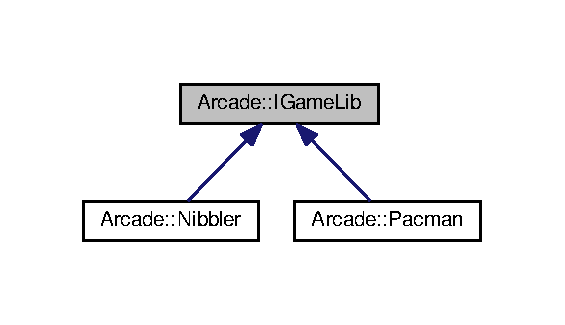
\includegraphics[width=271pt]{class_arcade_1_1_i_game_lib__inherit__graph}
\end{center}
\end{figure}
\subsection*{Public Member Functions}
\begin{DoxyCompactItemize}
\item 
virtual \hyperlink{class_arcade_1_1_i_game_lib_a3243f08b84930f3ff29d82d9a2a43582}{$\sim$\+I\+Game\+Lib} ()=default
\begin{DoxyCompactList}\small\item\em Destructor. \end{DoxyCompactList}\item 
virtual const std\+::string \hyperlink{class_arcade_1_1_i_game_lib_afd2652d62ebfda4caa5d0c05ff40ed61}{get\+Name} () const =0
\begin{DoxyCompactList}\small\item\em Game name\textquotesingle{}s getter. \end{DoxyCompactList}\item 
virtual bool \hyperlink{class_arcade_1_1_i_game_lib_aacc4169a98dfeb007bcaf9dfeece9e08}{init} ()=0
\begin{DoxyCompactList}\small\item\em Init the resources needed by the game to run. \end{DoxyCompactList}\item 
virtual bool \hyperlink{class_arcade_1_1_i_game_lib_ab9b7c1bbbea1b86e8515e8fd188fe9cb}{stop} ()=0
\begin{DoxyCompactList}\small\item\em Unloads the library. \end{DoxyCompactList}\item 
virtual bool \hyperlink{class_arcade_1_1_i_game_lib_a3b1b66ec00899b4c9efcd6151bf2497e}{apply\+Event} (\hyperlink{namespace_arcade_a9b501908b20bc993e4f8226db5323c41}{Arcade\+::\+Keys} key)=0
\begin{DoxyCompactList}\small\item\em Processes the key obtained by the \hyperlink{class_arcade_1_1_i_graphic_lib}{I\+Graphic\+Lib} from the user to update the game state. \end{DoxyCompactList}\item 
virtual bool \hyperlink{class_arcade_1_1_i_game_lib_a0be7ffaa269e2fa47146bf27ad2c511a}{update} ()=0
\begin{DoxyCompactList}\small\item\em Updates the game state. \end{DoxyCompactList}\item 
virtual void \hyperlink{class_arcade_1_1_i_game_lib_a00c3d335ef313e441217b33dcf7844df}{refresh} (\hyperlink{class_arcade_1_1_i_graphic_lib}{I\+Graphic\+Lib} \&graphic\+Lib)=0
\item 
virtual size\+\_\+t \hyperlink{class_arcade_1_1_i_game_lib_a00cdcad68c670aecbcc249a2995833b6}{get\+Score} ()=0
\begin{DoxyCompactList}\small\item\em Current player score\textquotesingle{}s getter. \end{DoxyCompactList}\end{DoxyCompactItemize}


\subsection{Detailed Description}
Game libraries virtual class. 

Purely virtual class that serves as the basis for all game libraries 

\subsection{Constructor \& Destructor Documentation}
\mbox{\Hypertarget{class_arcade_1_1_i_game_lib_a3243f08b84930f3ff29d82d9a2a43582}\label{class_arcade_1_1_i_game_lib_a3243f08b84930f3ff29d82d9a2a43582}} 
\index{Arcade\+::\+I\+Game\+Lib@{Arcade\+::\+I\+Game\+Lib}!````~I\+Game\+Lib@{$\sim$\+I\+Game\+Lib}}
\index{````~I\+Game\+Lib@{$\sim$\+I\+Game\+Lib}!Arcade\+::\+I\+Game\+Lib@{Arcade\+::\+I\+Game\+Lib}}
\subsubsection{\texorpdfstring{$\sim$\+I\+Game\+Lib()}{~IGameLib()}}
{\footnotesize\ttfamily virtual Arcade\+::\+I\+Game\+Lib\+::$\sim$\+I\+Game\+Lib (\begin{DoxyParamCaption}{ }\end{DoxyParamCaption})\hspace{0.3cm}{\ttfamily [virtual]}, {\ttfamily [default]}}



Destructor. 

\hyperlink{class_arcade_1_1_i_game_lib}{I\+Game\+Lib} class\textquotesingle{}s destructor 

\subsection{Member Function Documentation}
\mbox{\Hypertarget{class_arcade_1_1_i_game_lib_a3b1b66ec00899b4c9efcd6151bf2497e}\label{class_arcade_1_1_i_game_lib_a3b1b66ec00899b4c9efcd6151bf2497e}} 
\index{Arcade\+::\+I\+Game\+Lib@{Arcade\+::\+I\+Game\+Lib}!apply\+Event@{apply\+Event}}
\index{apply\+Event@{apply\+Event}!Arcade\+::\+I\+Game\+Lib@{Arcade\+::\+I\+Game\+Lib}}
\subsubsection{\texorpdfstring{apply\+Event()}{applyEvent()}}
{\footnotesize\ttfamily virtual bool Arcade\+::\+I\+Game\+Lib\+::apply\+Event (\begin{DoxyParamCaption}\item[{\hyperlink{namespace_arcade_a9b501908b20bc993e4f8226db5323c41}{Arcade\+::\+Keys}}]{key }\end{DoxyParamCaption})\hspace{0.3cm}{\ttfamily [pure virtual]}}



Processes the key obtained by the \hyperlink{class_arcade_1_1_i_graphic_lib}{I\+Graphic\+Lib} from the user to update the game state. 


\begin{DoxyParams}{Parameters}
{\em key} & \+: enum value of the obtained key \\
\hline
\end{DoxyParams}
\begin{DoxyReturn}{Returns}
true if the game is still in progress, false in case of defeat 
\end{DoxyReturn}


Implemented in \hyperlink{class_arcade_1_1_nibbler_a979cdf9080be6cb60bf1b4e757029845}{Arcade\+::\+Nibbler}, and \hyperlink{class_arcade_1_1_pacman_ac5fa3a4d5eaa81d37e8b63451265870d}{Arcade\+::\+Pacman}.

\mbox{\Hypertarget{class_arcade_1_1_i_game_lib_afd2652d62ebfda4caa5d0c05ff40ed61}\label{class_arcade_1_1_i_game_lib_afd2652d62ebfda4caa5d0c05ff40ed61}} 
\index{Arcade\+::\+I\+Game\+Lib@{Arcade\+::\+I\+Game\+Lib}!get\+Name@{get\+Name}}
\index{get\+Name@{get\+Name}!Arcade\+::\+I\+Game\+Lib@{Arcade\+::\+I\+Game\+Lib}}
\subsubsection{\texorpdfstring{get\+Name()}{getName()}}
{\footnotesize\ttfamily virtual const std\+::string Arcade\+::\+I\+Game\+Lib\+::get\+Name (\begin{DoxyParamCaption}{ }\end{DoxyParamCaption}) const\hspace{0.3cm}{\ttfamily [pure virtual]}}



Game name\textquotesingle{}s getter. 

\begin{DoxyReturn}{Returns}
a string containing the name of the game 
\end{DoxyReturn}


Implemented in \hyperlink{class_arcade_1_1_nibbler_abbd3cd2246448056bc84b5b893f325d4}{Arcade\+::\+Nibbler}, and \hyperlink{class_arcade_1_1_pacman_abc48d59a534276889f45128fe877d5d9}{Arcade\+::\+Pacman}.

\mbox{\Hypertarget{class_arcade_1_1_i_game_lib_a00cdcad68c670aecbcc249a2995833b6}\label{class_arcade_1_1_i_game_lib_a00cdcad68c670aecbcc249a2995833b6}} 
\index{Arcade\+::\+I\+Game\+Lib@{Arcade\+::\+I\+Game\+Lib}!get\+Score@{get\+Score}}
\index{get\+Score@{get\+Score}!Arcade\+::\+I\+Game\+Lib@{Arcade\+::\+I\+Game\+Lib}}
\subsubsection{\texorpdfstring{get\+Score()}{getScore()}}
{\footnotesize\ttfamily virtual size\+\_\+t Arcade\+::\+I\+Game\+Lib\+::get\+Score (\begin{DoxyParamCaption}{ }\end{DoxyParamCaption})\hspace{0.3cm}{\ttfamily [pure virtual]}}



Current player score\textquotesingle{}s getter. 

\begin{DoxyReturn}{Returns}
the player score
\end{DoxyReturn}
To call at the end of the execution of the game (after the player loose or win) for getting his score 

Implemented in \hyperlink{class_arcade_1_1_nibbler_a861f3bebe3b7f5efe1f3a46eb71957bb}{Arcade\+::\+Nibbler}, and \hyperlink{class_arcade_1_1_pacman_a7683729dd33fb18673c4d77764ca1831}{Arcade\+::\+Pacman}.

\mbox{\Hypertarget{class_arcade_1_1_i_game_lib_aacc4169a98dfeb007bcaf9dfeece9e08}\label{class_arcade_1_1_i_game_lib_aacc4169a98dfeb007bcaf9dfeece9e08}} 
\index{Arcade\+::\+I\+Game\+Lib@{Arcade\+::\+I\+Game\+Lib}!init@{init}}
\index{init@{init}!Arcade\+::\+I\+Game\+Lib@{Arcade\+::\+I\+Game\+Lib}}
\subsubsection{\texorpdfstring{init()}{init()}}
{\footnotesize\ttfamily virtual bool Arcade\+::\+I\+Game\+Lib\+::init (\begin{DoxyParamCaption}{ }\end{DoxyParamCaption})\hspace{0.3cm}{\ttfamily [pure virtual]}}



Init the resources needed by the game to run. 

\begin{DoxyReturn}{Returns}
true if succeed, otherwise returns false 
\end{DoxyReturn}


Implemented in \hyperlink{class_arcade_1_1_nibbler_a244e3c4751d74cab7e4e6ef7b80d0b36}{Arcade\+::\+Nibbler}, and \hyperlink{class_arcade_1_1_pacman_a27b0ecc843707c735ed1b65e7da009e1}{Arcade\+::\+Pacman}.

\mbox{\Hypertarget{class_arcade_1_1_i_game_lib_a00c3d335ef313e441217b33dcf7844df}\label{class_arcade_1_1_i_game_lib_a00c3d335ef313e441217b33dcf7844df}} 
\index{Arcade\+::\+I\+Game\+Lib@{Arcade\+::\+I\+Game\+Lib}!refresh@{refresh}}
\index{refresh@{refresh}!Arcade\+::\+I\+Game\+Lib@{Arcade\+::\+I\+Game\+Lib}}
\subsubsection{\texorpdfstring{refresh()}{refresh()}}
{\footnotesize\ttfamily virtual void Arcade\+::\+I\+Game\+Lib\+::refresh (\begin{DoxyParamCaption}\item[{\hyperlink{class_arcade_1_1_i_graphic_lib}{I\+Graphic\+Lib} \&}]{graphic\+Lib }\end{DoxyParamCaption})\hspace{0.3cm}{\ttfamily [pure virtual]}}

Renders the game state to the screen. 
\begin{DoxyParams}{Parameters}
{\em graphic\+Lib} & \+: Loaded graphics library used for rendering.\\
\hline
\end{DoxyParams}
This should call I\+Graphic\+Lib\+::refresh() to display content to the user. 

Implemented in \hyperlink{class_arcade_1_1_nibbler_a69a64ec51964772a03cf7d4bb9088b5b}{Arcade\+::\+Nibbler}, and \hyperlink{class_arcade_1_1_pacman_ad0d57afab410c98d4050c030b06ad63a}{Arcade\+::\+Pacman}.

\mbox{\Hypertarget{class_arcade_1_1_i_game_lib_ab9b7c1bbbea1b86e8515e8fd188fe9cb}\label{class_arcade_1_1_i_game_lib_ab9b7c1bbbea1b86e8515e8fd188fe9cb}} 
\index{Arcade\+::\+I\+Game\+Lib@{Arcade\+::\+I\+Game\+Lib}!stop@{stop}}
\index{stop@{stop}!Arcade\+::\+I\+Game\+Lib@{Arcade\+::\+I\+Game\+Lib}}
\subsubsection{\texorpdfstring{stop()}{stop()}}
{\footnotesize\ttfamily virtual bool Arcade\+::\+I\+Game\+Lib\+::stop (\begin{DoxyParamCaption}{ }\end{DoxyParamCaption})\hspace{0.3cm}{\ttfamily [pure virtual]}}



Unloads the library. 

\begin{DoxyReturn}{Returns}
true if succeed, otherwise returns false 
\end{DoxyReturn}


Implemented in \hyperlink{class_arcade_1_1_nibbler_ab88c7e92e23e603b6bd1ccbb6c1ab844}{Arcade\+::\+Nibbler}, and \hyperlink{class_arcade_1_1_pacman_a2787800feab139ddeabb11d6ee23a80e}{Arcade\+::\+Pacman}.

\mbox{\Hypertarget{class_arcade_1_1_i_game_lib_a0be7ffaa269e2fa47146bf27ad2c511a}\label{class_arcade_1_1_i_game_lib_a0be7ffaa269e2fa47146bf27ad2c511a}} 
\index{Arcade\+::\+I\+Game\+Lib@{Arcade\+::\+I\+Game\+Lib}!update@{update}}
\index{update@{update}!Arcade\+::\+I\+Game\+Lib@{Arcade\+::\+I\+Game\+Lib}}
\subsubsection{\texorpdfstring{update()}{update()}}
{\footnotesize\ttfamily virtual bool Arcade\+::\+I\+Game\+Lib\+::update (\begin{DoxyParamCaption}{ }\end{DoxyParamCaption})\hspace{0.3cm}{\ttfamily [pure virtual]}}



Updates the game state. 

\begin{DoxyReturn}{Returns}
true if the game is still in progress, false in case of defeat
\end{DoxyReturn}
Move the player forward and/or move the N\+P\+Cs, according to the game\textquotesingle{}s rules 

Implemented in \hyperlink{class_arcade_1_1_nibbler_a13199140bc927065b1c59ae2c70e06cf}{Arcade\+::\+Nibbler}, and \hyperlink{class_arcade_1_1_pacman_aacb11530e954870a6939d91794cbe356}{Arcade\+::\+Pacman}.



The documentation for this class was generated from the following file\+:\begin{DoxyCompactItemize}
\item 
/home/rectoria/projects/epitech/\+C\+P\+P/cpp\+\_\+arcade/interfaces/\hyperlink{_i_game_lib_8hpp}{I\+Game\+Lib.\+hpp}\end{DoxyCompactItemize}

\hypertarget{class_arcade_1_1_i_graphic_lib}{}\section{Arcade\+:\+:I\+Graphic\+Lib Class Reference}
\label{class_arcade_1_1_i_graphic_lib}\index{Arcade\+::\+I\+Graphic\+Lib@{Arcade\+::\+I\+Graphic\+Lib}}


Graphic libraries virtual class.  




{\ttfamily \#include $<$I\+Graphic\+Lib.\+hpp$>$}



Inheritance diagram for Arcade\+:\+:I\+Graphic\+Lib\+:
\nopagebreak
\begin{figure}[H]
\begin{center}
\leavevmode
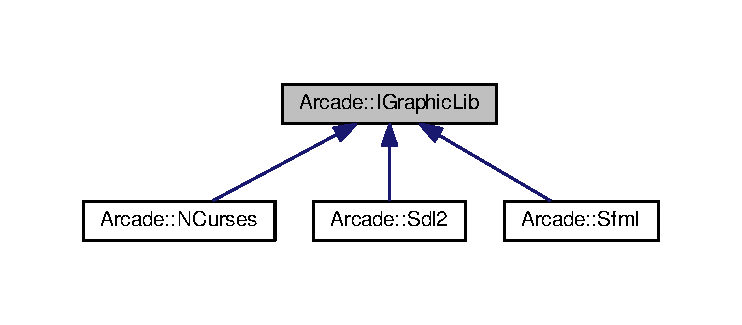
\includegraphics[width=350pt]{class_arcade_1_1_i_graphic_lib__inherit__graph}
\end{center}
\end{figure}
\subsection*{Public Member Functions}
\begin{DoxyCompactItemize}
\item 
virtual \hyperlink{class_arcade_1_1_i_graphic_lib_a57fc39424aebb606cc64ee8d7e40afd5}{$\sim$\+I\+Graphic\+Lib} ()=default
\begin{DoxyCompactList}\small\item\em Destructor. \end{DoxyCompactList}\item 
virtual std\+::string \hyperlink{class_arcade_1_1_i_graphic_lib_aecc266c4ac10f07f4cdca023e74e843d}{get\+Name} () const =0
\begin{DoxyCompactList}\small\item\em Graphic library name\textquotesingle{}s getter. \end{DoxyCompactList}\item 
virtual bool \hyperlink{class_arcade_1_1_i_graphic_lib_adf9e107fbcfbd91e5a3daa9a2db76b4b}{is\+Open} () const =0
\begin{DoxyCompactList}\small\item\em Specifies whether the window is open or not. \end{DoxyCompactList}\item 
virtual void \hyperlink{class_arcade_1_1_i_graphic_lib_aa7c3c8b922fbc94f5e74ecfebad52742}{close\+Renderer} ()=0
\begin{DoxyCompactList}\small\item\em Closes the rendering support. \end{DoxyCompactList}\item 
virtual void \hyperlink{class_arcade_1_1_i_graphic_lib_a71f7f51bdd61b02377c4a9ec330eabb1}{open\+Renderer} (std\+::string const \&title)=0
\begin{DoxyCompactList}\small\item\em Opens the rendering support. \end{DoxyCompactList}\item 
\mbox{\Hypertarget{class_arcade_1_1_i_graphic_lib_a24be73062bfc9bb79f7656568cc744d5}\label{class_arcade_1_1_i_graphic_lib_a24be73062bfc9bb79f7656568cc744d5}} 
virtual void \hyperlink{class_arcade_1_1_i_graphic_lib_a24be73062bfc9bb79f7656568cc744d5}{clear\+Window} ()=0
\begin{DoxyCompactList}\small\item\em Clears the rendering support. \end{DoxyCompactList}\item 
\mbox{\Hypertarget{class_arcade_1_1_i_graphic_lib_a58246883702914f057d36de24a33f8e1}\label{class_arcade_1_1_i_graphic_lib_a58246883702914f057d36de24a33f8e1}} 
virtual void \hyperlink{class_arcade_1_1_i_graphic_lib_a58246883702914f057d36de24a33f8e1}{refresh\+Window} ()=0
\begin{DoxyCompactList}\small\item\em Displays the buffered frame to the screen. \end{DoxyCompactList}\item 
\mbox{\Hypertarget{class_arcade_1_1_i_graphic_lib_af183213a30dacc943d32027cb784fe93}\label{class_arcade_1_1_i_graphic_lib_af183213a30dacc943d32027cb784fe93}} 
virtual void \hyperlink{class_arcade_1_1_i_graphic_lib_af183213a30dacc943d32027cb784fe93}{draw\+Pixel\+Box} (\hyperlink{class_arcade_1_1_pixel_box}{Pixel\+Box} const \&)=0
\begin{DoxyCompactList}\small\item\em Draws a \hyperlink{class_arcade_1_1_pixel_box}{Pixel\+Box}. \end{DoxyCompactList}\item 
\mbox{\Hypertarget{class_arcade_1_1_i_graphic_lib_aae06f5719d6557d70c1c4f7ec5acf9c3}\label{class_arcade_1_1_i_graphic_lib_aae06f5719d6557d70c1c4f7ec5acf9c3}} 
virtual void \hyperlink{class_arcade_1_1_i_graphic_lib_aae06f5719d6557d70c1c4f7ec5acf9c3}{draw\+Text} (\hyperlink{class_arcade_1_1_text_box}{Text\+Box} const \&)=0
\begin{DoxyCompactList}\small\item\em Draws a \hyperlink{class_arcade_1_1_text_box}{Text\+Box}. \end{DoxyCompactList}\item 
virtual bool \hyperlink{class_arcade_1_1_i_graphic_lib_a6be852f0395f08943f988c6823b80937}{poll\+Events} ()=0
\begin{DoxyCompactList}\small\item\em Fetches the events from the user and saves it. \end{DoxyCompactList}\item 
virtual \hyperlink{namespace_arcade_a9b501908b20bc993e4f8226db5323c41}{Keys} \hyperlink{class_arcade_1_1_i_graphic_lib_a801ebd3cff2c861e4b2a1e664c123da7}{get\+Last\+Event} ()=0
\begin{DoxyCompactList}\small\item\em Getter of the oldest command in memory. \end{DoxyCompactList}\item 
virtual void \hyperlink{class_arcade_1_1_i_graphic_lib_a78691f8f9433b2af945576231534c1e3}{clear\+Events} ()=0
\begin{DoxyCompactList}\small\item\em Clears the pending commands. \end{DoxyCompactList}\item 
virtual \hyperlink{class_arcade_1_1_vect}{Vect}$<$ size\+\_\+t $>$ \hyperlink{class_arcade_1_1_i_graphic_lib_a0ce5eb4661d55b6e729fc1c16566dd9f}{get\+Screen\+Size} () const =0
\begin{DoxyCompactList}\small\item\em Getter from the rendering support dimensions. \end{DoxyCompactList}\item 
virtual size\+\_\+t \hyperlink{class_arcade_1_1_i_graphic_lib_ae8701e702b51189c84b1900dd624912e}{get\+MaxY} () const =0
\begin{DoxyCompactList}\small\item\em Getter from the rendering support height. \end{DoxyCompactList}\item 
virtual size\+\_\+t \hyperlink{class_arcade_1_1_i_graphic_lib_a41a3c00970ecd16e1893105de2091a55}{get\+MaxX} () const =0
\begin{DoxyCompactList}\small\item\em Getter from the rendering support width. \end{DoxyCompactList}\end{DoxyCompactItemize}


\subsection{Detailed Description}
Graphic libraries virtual class. 

Purely virtual class that serves as the basis for all graphic libraries 

\subsection{Constructor \& Destructor Documentation}
\mbox{\Hypertarget{class_arcade_1_1_i_graphic_lib_a57fc39424aebb606cc64ee8d7e40afd5}\label{class_arcade_1_1_i_graphic_lib_a57fc39424aebb606cc64ee8d7e40afd5}} 
\index{Arcade\+::\+I\+Graphic\+Lib@{Arcade\+::\+I\+Graphic\+Lib}!````~I\+Graphic\+Lib@{$\sim$\+I\+Graphic\+Lib}}
\index{````~I\+Graphic\+Lib@{$\sim$\+I\+Graphic\+Lib}!Arcade\+::\+I\+Graphic\+Lib@{Arcade\+::\+I\+Graphic\+Lib}}
\subsubsection{\texorpdfstring{$\sim$\+I\+Graphic\+Lib()}{~IGraphicLib()}}
{\footnotesize\ttfamily virtual Arcade\+::\+I\+Graphic\+Lib\+::$\sim$\+I\+Graphic\+Lib (\begin{DoxyParamCaption}{ }\end{DoxyParamCaption})\hspace{0.3cm}{\ttfamily [virtual]}, {\ttfamily [default]}}



Destructor. 

\hyperlink{class_arcade_1_1_i_graphic_lib}{I\+Graphic\+Lib} class\textquotesingle{}s destructor 

\subsection{Member Function Documentation}
\mbox{\Hypertarget{class_arcade_1_1_i_graphic_lib_a78691f8f9433b2af945576231534c1e3}\label{class_arcade_1_1_i_graphic_lib_a78691f8f9433b2af945576231534c1e3}} 
\index{Arcade\+::\+I\+Graphic\+Lib@{Arcade\+::\+I\+Graphic\+Lib}!clear\+Events@{clear\+Events}}
\index{clear\+Events@{clear\+Events}!Arcade\+::\+I\+Graphic\+Lib@{Arcade\+::\+I\+Graphic\+Lib}}
\subsubsection{\texorpdfstring{clear\+Events()}{clearEvents()}}
{\footnotesize\ttfamily virtual void Arcade\+::\+I\+Graphic\+Lib\+::clear\+Events (\begin{DoxyParamCaption}{ }\end{DoxyParamCaption})\hspace{0.3cm}{\ttfamily [pure virtual]}}



Clears the pending commands. 

The function deletes all the commands currently stored. They wont be accessible anymore, even with the \hyperlink{class_arcade_1_1_i_graphic_lib_a801ebd3cff2c861e4b2a1e664c123da7}{get\+Last\+Event()} method. 

Implemented in \hyperlink{class_arcade_1_1_n_curses_a01dd738afe5e5546e165b911091b32cc}{Arcade\+::\+N\+Curses}, \hyperlink{class_arcade_1_1_sfml_a882877eba4037ffe3befd61a4b4f1d18}{Arcade\+::\+Sfml}, and \hyperlink{class_arcade_1_1_sdl2_a92f016d43686b195673aea7f3446d0a1}{Arcade\+::\+Sdl2}.

\mbox{\Hypertarget{class_arcade_1_1_i_graphic_lib_aa7c3c8b922fbc94f5e74ecfebad52742}\label{class_arcade_1_1_i_graphic_lib_aa7c3c8b922fbc94f5e74ecfebad52742}} 
\index{Arcade\+::\+I\+Graphic\+Lib@{Arcade\+::\+I\+Graphic\+Lib}!close\+Renderer@{close\+Renderer}}
\index{close\+Renderer@{close\+Renderer}!Arcade\+::\+I\+Graphic\+Lib@{Arcade\+::\+I\+Graphic\+Lib}}
\subsubsection{\texorpdfstring{close\+Renderer()}{closeRenderer()}}
{\footnotesize\ttfamily virtual void Arcade\+::\+I\+Graphic\+Lib\+::close\+Renderer (\begin{DoxyParamCaption}{ }\end{DoxyParamCaption})\hspace{0.3cm}{\ttfamily [pure virtual]}}



Closes the rendering support. 

Usually closes a window. Some graphic library uses other rendering support. 

Implemented in \hyperlink{class_arcade_1_1_n_curses_a1bbac59bdaa841d17439d01a06d9f5c3}{Arcade\+::\+N\+Curses}, \hyperlink{class_arcade_1_1_sfml_a3a2c22328c9ae1cfd7a5af03663e00d0}{Arcade\+::\+Sfml}, and \hyperlink{class_arcade_1_1_sdl2_a312397e628bbf14d8532e2a13575c7ab}{Arcade\+::\+Sdl2}.

\mbox{\Hypertarget{class_arcade_1_1_i_graphic_lib_a801ebd3cff2c861e4b2a1e664c123da7}\label{class_arcade_1_1_i_graphic_lib_a801ebd3cff2c861e4b2a1e664c123da7}} 
\index{Arcade\+::\+I\+Graphic\+Lib@{Arcade\+::\+I\+Graphic\+Lib}!get\+Last\+Event@{get\+Last\+Event}}
\index{get\+Last\+Event@{get\+Last\+Event}!Arcade\+::\+I\+Graphic\+Lib@{Arcade\+::\+I\+Graphic\+Lib}}
\subsubsection{\texorpdfstring{get\+Last\+Event()}{getLastEvent()}}
{\footnotesize\ttfamily virtual \hyperlink{namespace_arcade_a9b501908b20bc993e4f8226db5323c41}{Keys} Arcade\+::\+I\+Graphic\+Lib\+::get\+Last\+Event (\begin{DoxyParamCaption}{ }\end{DoxyParamCaption})\hspace{0.3cm}{\ttfamily [pure virtual]}}



Getter of the oldest command in memory. 

\begin{DoxyReturn}{Returns}
the first event of the list.
\end{DoxyReturn}
The function deletes the command if it succeed to retrieves one, using front() and pop\+\_\+front() methods 

Implemented in \hyperlink{class_arcade_1_1_n_curses_a0c00b4aede0c9345f525fcb812fe8f78}{Arcade\+::\+N\+Curses}, \hyperlink{class_arcade_1_1_sfml_aa31ab4c4729ee0e3ff030989bc38237b}{Arcade\+::\+Sfml}, and \hyperlink{class_arcade_1_1_sdl2_a6d5bda09e7705c6ccef7451694621247}{Arcade\+::\+Sdl2}.

\mbox{\Hypertarget{class_arcade_1_1_i_graphic_lib_a41a3c00970ecd16e1893105de2091a55}\label{class_arcade_1_1_i_graphic_lib_a41a3c00970ecd16e1893105de2091a55}} 
\index{Arcade\+::\+I\+Graphic\+Lib@{Arcade\+::\+I\+Graphic\+Lib}!get\+MaxX@{get\+MaxX}}
\index{get\+MaxX@{get\+MaxX}!Arcade\+::\+I\+Graphic\+Lib@{Arcade\+::\+I\+Graphic\+Lib}}
\subsubsection{\texorpdfstring{get\+Max\+X()}{getMaxX()}}
{\footnotesize\ttfamily virtual size\+\_\+t Arcade\+::\+I\+Graphic\+Lib\+::get\+MaxX (\begin{DoxyParamCaption}{ }\end{DoxyParamCaption}) const\hspace{0.3cm}{\ttfamily [pure virtual]}}



Getter from the rendering support width. 

\begin{DoxyReturn}{Returns}
the width of the rendering support 
\end{DoxyReturn}


Implemented in \hyperlink{class_arcade_1_1_n_curses_a9f561bd405af76689763819794382ef1}{Arcade\+::\+N\+Curses}, \hyperlink{class_arcade_1_1_sfml_a220fc84bb5728f79e36024fded0103ab}{Arcade\+::\+Sfml}, and \hyperlink{class_arcade_1_1_sdl2_a9e9e70db8a77c2dee10e2227c70415e3}{Arcade\+::\+Sdl2}.

\mbox{\Hypertarget{class_arcade_1_1_i_graphic_lib_ae8701e702b51189c84b1900dd624912e}\label{class_arcade_1_1_i_graphic_lib_ae8701e702b51189c84b1900dd624912e}} 
\index{Arcade\+::\+I\+Graphic\+Lib@{Arcade\+::\+I\+Graphic\+Lib}!get\+MaxY@{get\+MaxY}}
\index{get\+MaxY@{get\+MaxY}!Arcade\+::\+I\+Graphic\+Lib@{Arcade\+::\+I\+Graphic\+Lib}}
\subsubsection{\texorpdfstring{get\+Max\+Y()}{getMaxY()}}
{\footnotesize\ttfamily virtual size\+\_\+t Arcade\+::\+I\+Graphic\+Lib\+::get\+MaxY (\begin{DoxyParamCaption}{ }\end{DoxyParamCaption}) const\hspace{0.3cm}{\ttfamily [pure virtual]}}



Getter from the rendering support height. 

\begin{DoxyReturn}{Returns}
the height of the rendering support 
\end{DoxyReturn}


Implemented in \hyperlink{class_arcade_1_1_n_curses_a00c879117a1de6752acd376bfd59e94d}{Arcade\+::\+N\+Curses}, \hyperlink{class_arcade_1_1_sfml_a90cb12cc852a0198074f55be843d6f99}{Arcade\+::\+Sfml}, and \hyperlink{class_arcade_1_1_sdl2_a958b3611cb0f7db90eeca5c9c4eaed59}{Arcade\+::\+Sdl2}.

\mbox{\Hypertarget{class_arcade_1_1_i_graphic_lib_aecc266c4ac10f07f4cdca023e74e843d}\label{class_arcade_1_1_i_graphic_lib_aecc266c4ac10f07f4cdca023e74e843d}} 
\index{Arcade\+::\+I\+Graphic\+Lib@{Arcade\+::\+I\+Graphic\+Lib}!get\+Name@{get\+Name}}
\index{get\+Name@{get\+Name}!Arcade\+::\+I\+Graphic\+Lib@{Arcade\+::\+I\+Graphic\+Lib}}
\subsubsection{\texorpdfstring{get\+Name()}{getName()}}
{\footnotesize\ttfamily virtual std\+::string Arcade\+::\+I\+Graphic\+Lib\+::get\+Name (\begin{DoxyParamCaption}{ }\end{DoxyParamCaption}) const\hspace{0.3cm}{\ttfamily [pure virtual]}}



Graphic library name\textquotesingle{}s getter. 

\begin{DoxyReturn}{Returns}
a string containing the name of the graphic library 
\end{DoxyReturn}


Implemented in \hyperlink{class_arcade_1_1_n_curses_a8674fcd61c00e65897db3435f31dfcc2}{Arcade\+::\+N\+Curses}, \hyperlink{class_arcade_1_1_sfml_a6c5776e27ea7466208ab4bd59395e344}{Arcade\+::\+Sfml}, and \hyperlink{class_arcade_1_1_sdl2_aa1d9e278616747b87d868fadb0272d43}{Arcade\+::\+Sdl2}.

\mbox{\Hypertarget{class_arcade_1_1_i_graphic_lib_a0ce5eb4661d55b6e729fc1c16566dd9f}\label{class_arcade_1_1_i_graphic_lib_a0ce5eb4661d55b6e729fc1c16566dd9f}} 
\index{Arcade\+::\+I\+Graphic\+Lib@{Arcade\+::\+I\+Graphic\+Lib}!get\+Screen\+Size@{get\+Screen\+Size}}
\index{get\+Screen\+Size@{get\+Screen\+Size}!Arcade\+::\+I\+Graphic\+Lib@{Arcade\+::\+I\+Graphic\+Lib}}
\subsubsection{\texorpdfstring{get\+Screen\+Size()}{getScreenSize()}}
{\footnotesize\ttfamily virtual \hyperlink{class_arcade_1_1_vect}{Vect}$<$size\+\_\+t$>$ Arcade\+::\+I\+Graphic\+Lib\+::get\+Screen\+Size (\begin{DoxyParamCaption}{ }\end{DoxyParamCaption}) const\hspace{0.3cm}{\ttfamily [pure virtual]}}



Getter from the rendering support dimensions. 

\begin{DoxyReturn}{Returns}
a two dimensions vector containing the width and the height of the rendering support 
\end{DoxyReturn}


Implemented in \hyperlink{class_arcade_1_1_n_curses_ae7a4eb70b4a07dc2d65f135c6f7ceb50}{Arcade\+::\+N\+Curses}, \hyperlink{class_arcade_1_1_sfml_aa2fe7257182649ba0273712d36296460}{Arcade\+::\+Sfml}, and \hyperlink{class_arcade_1_1_sdl2_ae54d60076b915de4fce36ace576ea01d}{Arcade\+::\+Sdl2}.

\mbox{\Hypertarget{class_arcade_1_1_i_graphic_lib_adf9e107fbcfbd91e5a3daa9a2db76b4b}\label{class_arcade_1_1_i_graphic_lib_adf9e107fbcfbd91e5a3daa9a2db76b4b}} 
\index{Arcade\+::\+I\+Graphic\+Lib@{Arcade\+::\+I\+Graphic\+Lib}!is\+Open@{is\+Open}}
\index{is\+Open@{is\+Open}!Arcade\+::\+I\+Graphic\+Lib@{Arcade\+::\+I\+Graphic\+Lib}}
\subsubsection{\texorpdfstring{is\+Open()}{isOpen()}}
{\footnotesize\ttfamily virtual bool Arcade\+::\+I\+Graphic\+Lib\+::is\+Open (\begin{DoxyParamCaption}{ }\end{DoxyParamCaption}) const\hspace{0.3cm}{\ttfamily [pure virtual]}}



Specifies whether the window is open or not. 

\begin{DoxyReturn}{Returns}
true if open, otherwise returns false 
\end{DoxyReturn}


Implemented in \hyperlink{class_arcade_1_1_n_curses_a04a81ada3532d84f6369479c0779dd1a}{Arcade\+::\+N\+Curses}, \hyperlink{class_arcade_1_1_sfml_a427b6fc608c3b52f167b1fe79f5a5009}{Arcade\+::\+Sfml}, and \hyperlink{class_arcade_1_1_sdl2_a44772ea99509adde0a1c8779265ce260}{Arcade\+::\+Sdl2}.

\mbox{\Hypertarget{class_arcade_1_1_i_graphic_lib_a71f7f51bdd61b02377c4a9ec330eabb1}\label{class_arcade_1_1_i_graphic_lib_a71f7f51bdd61b02377c4a9ec330eabb1}} 
\index{Arcade\+::\+I\+Graphic\+Lib@{Arcade\+::\+I\+Graphic\+Lib}!open\+Renderer@{open\+Renderer}}
\index{open\+Renderer@{open\+Renderer}!Arcade\+::\+I\+Graphic\+Lib@{Arcade\+::\+I\+Graphic\+Lib}}
\subsubsection{\texorpdfstring{open\+Renderer()}{openRenderer()}}
{\footnotesize\ttfamily virtual void Arcade\+::\+I\+Graphic\+Lib\+::open\+Renderer (\begin{DoxyParamCaption}\item[{std\+::string const \&}]{title }\end{DoxyParamCaption})\hspace{0.3cm}{\ttfamily [pure virtual]}}



Opens the rendering support. 


\begin{DoxyParams}{Parameters}
{\em title} & \+: Title of the rendering support if supported\\
\hline
\end{DoxyParams}
Usually opens a window. Some graphic library uses other rendering support. 

Implemented in \hyperlink{class_arcade_1_1_n_curses_a2bebb6d17c26471866a4403c64cda006}{Arcade\+::\+N\+Curses}, \hyperlink{class_arcade_1_1_sfml_a9a868d1964ac2f24327329af971fdb57}{Arcade\+::\+Sfml}, and \hyperlink{class_arcade_1_1_sdl2_aa7000a687e79acf5e5ff99ae6e71194b}{Arcade\+::\+Sdl2}.

\mbox{\Hypertarget{class_arcade_1_1_i_graphic_lib_a6be852f0395f08943f988c6823b80937}\label{class_arcade_1_1_i_graphic_lib_a6be852f0395f08943f988c6823b80937}} 
\index{Arcade\+::\+I\+Graphic\+Lib@{Arcade\+::\+I\+Graphic\+Lib}!poll\+Events@{poll\+Events}}
\index{poll\+Events@{poll\+Events}!Arcade\+::\+I\+Graphic\+Lib@{Arcade\+::\+I\+Graphic\+Lib}}
\subsubsection{\texorpdfstring{poll\+Events()}{pollEvents()}}
{\footnotesize\ttfamily virtual bool Arcade\+::\+I\+Graphic\+Lib\+::poll\+Events (\begin{DoxyParamCaption}{ }\end{DoxyParamCaption})\hspace{0.3cm}{\ttfamily [pure virtual]}}



Fetches the events from the user and saves it. 

\begin{DoxyReturn}{Returns}
true if at least one command has been fetched, otherwise returns false
\end{DoxyReturn}
Fetched commands are usually stored inside a std\+::vector$<$\+Arcade\+::\+Keys$>$ or std\+::list$<$\+Arcade\+::\+Keys$>$ 

Implemented in \hyperlink{class_arcade_1_1_n_curses_ae250fb39f3e256bef0492fd54ebdaee7}{Arcade\+::\+N\+Curses}, \hyperlink{class_arcade_1_1_sfml_a7b5fe6ccf84db8b3f2897805c965e607}{Arcade\+::\+Sfml}, and \hyperlink{class_arcade_1_1_sdl2_af794699db9401d1be49566908ec7bced}{Arcade\+::\+Sdl2}.



The documentation for this class was generated from the following file\+:\begin{DoxyCompactItemize}
\item 
/home/rectoria/projects/epitech/\+C\+P\+P/cpp\+\_\+arcade/interfaces/\hyperlink{_i_graphic_lib_8hpp}{I\+Graphic\+Lib.\+hpp}\end{DoxyCompactItemize}

\hypertarget{class_arcade_1_1_menu}{}\section{Arcade\+:\+:Menu Class Reference}
\label{class_arcade_1_1_menu}\index{Arcade\+::\+Menu@{Arcade\+::\+Menu}}
\subsection*{Public Member Functions}
\begin{DoxyCompactItemize}
\item 
\mbox{\Hypertarget{class_arcade_1_1_menu_a4d9fe370dd6f54072c84cc6b42ba7548}\label{class_arcade_1_1_menu_a4d9fe370dd6f54072c84cc6b42ba7548}} 
void {\bfseries set\+Lists} (std\+::vector$<$ \hyperlink{class_d_l_loader}{D\+L\+Loader}$<$ \hyperlink{class_arcade_1_1_i_game_lib}{I\+Game\+Lib} $>$ $\ast$$>$ $\ast$, std\+::vector$<$ \hyperlink{class_d_l_loader}{D\+L\+Loader}$<$ \hyperlink{class_arcade_1_1_i_graphic_lib}{I\+Graphic\+Lib} $>$ $\ast$$>$ $\ast$)
\item 
\mbox{\Hypertarget{class_arcade_1_1_menu_a0b980a97e7f7b9eabe27ea7e422af634}\label{class_arcade_1_1_menu_a0b980a97e7f7b9eabe27ea7e422af634}} 
void {\bfseries refresh} (\hyperlink{class_arcade_1_1_i_graphic_lib}{I\+Graphic\+Lib} $\ast$, unsigned, \hyperlink{class_arcade_1_1_score}{Arcade\+::\+Score})
\item 
\mbox{\Hypertarget{class_arcade_1_1_menu_aec85eb1191a0f094c279485d49baa010}\label{class_arcade_1_1_menu_aec85eb1191a0f094c279485d49baa010}} 
unsigned {\bfseries apply\+Event} (\hyperlink{namespace_arcade_a9b501908b20bc993e4f8226db5323c41}{Keys})
\item 
\mbox{\Hypertarget{class_arcade_1_1_menu_a55e14b8d591a0cbfed3f89a3f8e35a80}\label{class_arcade_1_1_menu_a55e14b8d591a0cbfed3f89a3f8e35a80}} 
std\+::string {\bfseries get\+User\+Name} () const
\end{DoxyCompactItemize}


The documentation for this class was generated from the following files\+:\begin{DoxyCompactItemize}
\item 
/home/rectoria/projects/epitech/\+C\+P\+P/cpp\+\_\+arcade/src/menu/Menu.\+hpp\item 
/home/rectoria/projects/epitech/\+C\+P\+P/cpp\+\_\+arcade/src/menu/Menu.\+cpp\end{DoxyCompactItemize}

\hypertarget{class_arcade_1_1_n_curses}{}\section{Arcade\+:\+:N\+Curses Class Reference}
\label{class_arcade_1_1_n_curses}\index{Arcade\+::\+N\+Curses@{Arcade\+::\+N\+Curses}}


Inheritance diagram for Arcade\+:\+:N\+Curses\+:
\nopagebreak
\begin{figure}[H]
\begin{center}
\leavevmode
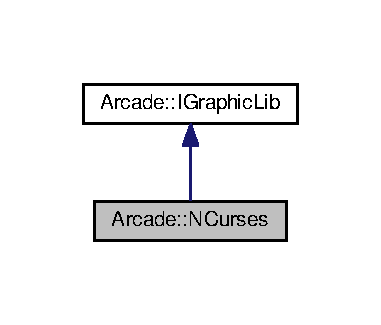
\includegraphics[width=183pt]{class_arcade_1_1_n_curses__inherit__graph}
\end{center}
\end{figure}


Collaboration diagram for Arcade\+:\+:N\+Curses\+:
\nopagebreak
\begin{figure}[H]
\begin{center}
\leavevmode
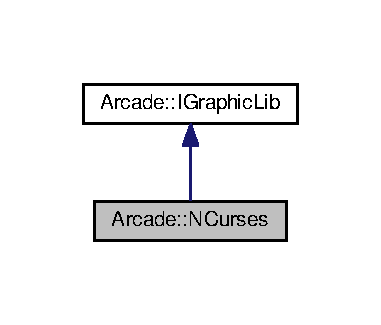
\includegraphics[width=183pt]{class_arcade_1_1_n_curses__coll__graph}
\end{center}
\end{figure}
\subsection*{Public Member Functions}
\begin{DoxyCompactItemize}
\item 
std\+::string \hyperlink{class_arcade_1_1_n_curses_a8674fcd61c00e65897db3435f31dfcc2}{get\+Name} () const final
\begin{DoxyCompactList}\small\item\em Graphic library name\textquotesingle{}s getter. \end{DoxyCompactList}\item 
bool \hyperlink{class_arcade_1_1_n_curses_a04a81ada3532d84f6369479c0779dd1a}{is\+Open} () const final
\begin{DoxyCompactList}\small\item\em Specifies whether the window is open or not. \end{DoxyCompactList}\item 
void \hyperlink{class_arcade_1_1_n_curses_a1bbac59bdaa841d17439d01a06d9f5c3}{close\+Renderer} () final
\begin{DoxyCompactList}\small\item\em Closes the rendering support. \end{DoxyCompactList}\item 
void \hyperlink{class_arcade_1_1_n_curses_a2bebb6d17c26471866a4403c64cda006}{open\+Renderer} (std\+::string const \&title) final
\begin{DoxyCompactList}\small\item\em Opens the rendering support. \end{DoxyCompactList}\item 
\mbox{\Hypertarget{class_arcade_1_1_n_curses_ad0d75bd7574c6d567c60106c66033307}\label{class_arcade_1_1_n_curses_ad0d75bd7574c6d567c60106c66033307}} 
void \hyperlink{class_arcade_1_1_n_curses_ad0d75bd7574c6d567c60106c66033307}{clear\+Window} () final
\begin{DoxyCompactList}\small\item\em Clears the rendering support. \end{DoxyCompactList}\item 
\mbox{\Hypertarget{class_arcade_1_1_n_curses_a380dff7e62958331765db70be5b76a64}\label{class_arcade_1_1_n_curses_a380dff7e62958331765db70be5b76a64}} 
void \hyperlink{class_arcade_1_1_n_curses_a380dff7e62958331765db70be5b76a64}{refresh\+Window} () final
\begin{DoxyCompactList}\small\item\em Displays the buffered frame to the screen. \end{DoxyCompactList}\item 
\mbox{\Hypertarget{class_arcade_1_1_n_curses_ad55a11d0661a5560bba131f7c4af3fde}\label{class_arcade_1_1_n_curses_ad55a11d0661a5560bba131f7c4af3fde}} 
void \hyperlink{class_arcade_1_1_n_curses_ad55a11d0661a5560bba131f7c4af3fde}{draw\+Pixel\+Box} (\hyperlink{class_arcade_1_1_pixel_box}{Pixel\+Box} const \&) final
\begin{DoxyCompactList}\small\item\em Draws a \hyperlink{class_arcade_1_1_pixel_box}{Pixel\+Box}. \end{DoxyCompactList}\item 
\mbox{\Hypertarget{class_arcade_1_1_n_curses_a97d6fdf07172465349c0f08fb9effede}\label{class_arcade_1_1_n_curses_a97d6fdf07172465349c0f08fb9effede}} 
void \hyperlink{class_arcade_1_1_n_curses_a97d6fdf07172465349c0f08fb9effede}{draw\+Text} (\hyperlink{class_arcade_1_1_text_box}{Text\+Box} const \&) final
\begin{DoxyCompactList}\small\item\em Draws a \hyperlink{class_arcade_1_1_text_box}{Text\+Box}. \end{DoxyCompactList}\item 
bool \hyperlink{class_arcade_1_1_n_curses_ae250fb39f3e256bef0492fd54ebdaee7}{poll\+Events} () final
\begin{DoxyCompactList}\small\item\em Fetches the events from the user and saves it. \end{DoxyCompactList}\item 
\hyperlink{namespace_arcade_a9b501908b20bc993e4f8226db5323c41}{Keys} \hyperlink{class_arcade_1_1_n_curses_a0c00b4aede0c9345f525fcb812fe8f78}{get\+Last\+Event} () final
\begin{DoxyCompactList}\small\item\em Getter of the oldest command in memory. \end{DoxyCompactList}\item 
void \hyperlink{class_arcade_1_1_n_curses_a01dd738afe5e5546e165b911091b32cc}{clear\+Events} () final
\begin{DoxyCompactList}\small\item\em Clears the pending commands. \end{DoxyCompactList}\item 
\hyperlink{class_arcade_1_1_vect}{Vect}$<$ size\+\_\+t $>$ \hyperlink{class_arcade_1_1_n_curses_ae7a4eb70b4a07dc2d65f135c6f7ceb50}{get\+Screen\+Size} () const final
\begin{DoxyCompactList}\small\item\em Getter from the rendering support dimensions. \end{DoxyCompactList}\item 
size\+\_\+t \hyperlink{class_arcade_1_1_n_curses_a00c879117a1de6752acd376bfd59e94d}{get\+MaxY} () const final
\begin{DoxyCompactList}\small\item\em Getter from the rendering support height. \end{DoxyCompactList}\item 
size\+\_\+t \hyperlink{class_arcade_1_1_n_curses_a9f561bd405af76689763819794382ef1}{get\+MaxX} () const final
\begin{DoxyCompactList}\small\item\em Getter from the rendering support width. \end{DoxyCompactList}\end{DoxyCompactItemize}


\subsection{Member Function Documentation}
\mbox{\Hypertarget{class_arcade_1_1_n_curses_a01dd738afe5e5546e165b911091b32cc}\label{class_arcade_1_1_n_curses_a01dd738afe5e5546e165b911091b32cc}} 
\index{Arcade\+::\+N\+Curses@{Arcade\+::\+N\+Curses}!clear\+Events@{clear\+Events}}
\index{clear\+Events@{clear\+Events}!Arcade\+::\+N\+Curses@{Arcade\+::\+N\+Curses}}
\subsubsection{\texorpdfstring{clear\+Events()}{clearEvents()}}
{\footnotesize\ttfamily void Arcade\+::\+N\+Curses\+::clear\+Events (\begin{DoxyParamCaption}{ }\end{DoxyParamCaption})\hspace{0.3cm}{\ttfamily [final]}, {\ttfamily [virtual]}}



Clears the pending commands. 

The function deletes all the commands currently stored. They wont be accessible anymore, even with the \hyperlink{class_arcade_1_1_n_curses_a0c00b4aede0c9345f525fcb812fe8f78}{get\+Last\+Event()} method. 

Implements \hyperlink{class_arcade_1_1_i_graphic_lib_a78691f8f9433b2af945576231534c1e3}{Arcade\+::\+I\+Graphic\+Lib}.

\mbox{\Hypertarget{class_arcade_1_1_n_curses_a1bbac59bdaa841d17439d01a06d9f5c3}\label{class_arcade_1_1_n_curses_a1bbac59bdaa841d17439d01a06d9f5c3}} 
\index{Arcade\+::\+N\+Curses@{Arcade\+::\+N\+Curses}!close\+Renderer@{close\+Renderer}}
\index{close\+Renderer@{close\+Renderer}!Arcade\+::\+N\+Curses@{Arcade\+::\+N\+Curses}}
\subsubsection{\texorpdfstring{close\+Renderer()}{closeRenderer()}}
{\footnotesize\ttfamily void Arcade\+::\+N\+Curses\+::close\+Renderer (\begin{DoxyParamCaption}{ }\end{DoxyParamCaption})\hspace{0.3cm}{\ttfamily [final]}, {\ttfamily [virtual]}}



Closes the rendering support. 

Usually closes a window. Some graphic library uses other rendering support. 

Implements \hyperlink{class_arcade_1_1_i_graphic_lib_aa7c3c8b922fbc94f5e74ecfebad52742}{Arcade\+::\+I\+Graphic\+Lib}.

\mbox{\Hypertarget{class_arcade_1_1_n_curses_a0c00b4aede0c9345f525fcb812fe8f78}\label{class_arcade_1_1_n_curses_a0c00b4aede0c9345f525fcb812fe8f78}} 
\index{Arcade\+::\+N\+Curses@{Arcade\+::\+N\+Curses}!get\+Last\+Event@{get\+Last\+Event}}
\index{get\+Last\+Event@{get\+Last\+Event}!Arcade\+::\+N\+Curses@{Arcade\+::\+N\+Curses}}
\subsubsection{\texorpdfstring{get\+Last\+Event()}{getLastEvent()}}
{\footnotesize\ttfamily \hyperlink{namespace_arcade_a9b501908b20bc993e4f8226db5323c41}{Arcade\+::\+Keys} Arcade\+::\+N\+Curses\+::get\+Last\+Event (\begin{DoxyParamCaption}{ }\end{DoxyParamCaption})\hspace{0.3cm}{\ttfamily [final]}, {\ttfamily [virtual]}}



Getter of the oldest command in memory. 

\begin{DoxyReturn}{Returns}
the first event of the list.
\end{DoxyReturn}
The function deletes the command if it succeed to retrieves one, using front() and pop\+\_\+front() methods 

Implements \hyperlink{class_arcade_1_1_i_graphic_lib_a801ebd3cff2c861e4b2a1e664c123da7}{Arcade\+::\+I\+Graphic\+Lib}.

\mbox{\Hypertarget{class_arcade_1_1_n_curses_a9f561bd405af76689763819794382ef1}\label{class_arcade_1_1_n_curses_a9f561bd405af76689763819794382ef1}} 
\index{Arcade\+::\+N\+Curses@{Arcade\+::\+N\+Curses}!get\+MaxX@{get\+MaxX}}
\index{get\+MaxX@{get\+MaxX}!Arcade\+::\+N\+Curses@{Arcade\+::\+N\+Curses}}
\subsubsection{\texorpdfstring{get\+Max\+X()}{getMaxX()}}
{\footnotesize\ttfamily size\+\_\+t Arcade\+::\+N\+Curses\+::get\+MaxX (\begin{DoxyParamCaption}{ }\end{DoxyParamCaption}) const\hspace{0.3cm}{\ttfamily [final]}, {\ttfamily [virtual]}}



Getter from the rendering support width. 

\begin{DoxyReturn}{Returns}
the width of the rendering support 
\end{DoxyReturn}


Implements \hyperlink{class_arcade_1_1_i_graphic_lib_a41a3c00970ecd16e1893105de2091a55}{Arcade\+::\+I\+Graphic\+Lib}.

\mbox{\Hypertarget{class_arcade_1_1_n_curses_a00c879117a1de6752acd376bfd59e94d}\label{class_arcade_1_1_n_curses_a00c879117a1de6752acd376bfd59e94d}} 
\index{Arcade\+::\+N\+Curses@{Arcade\+::\+N\+Curses}!get\+MaxY@{get\+MaxY}}
\index{get\+MaxY@{get\+MaxY}!Arcade\+::\+N\+Curses@{Arcade\+::\+N\+Curses}}
\subsubsection{\texorpdfstring{get\+Max\+Y()}{getMaxY()}}
{\footnotesize\ttfamily size\+\_\+t Arcade\+::\+N\+Curses\+::get\+MaxY (\begin{DoxyParamCaption}{ }\end{DoxyParamCaption}) const\hspace{0.3cm}{\ttfamily [final]}, {\ttfamily [virtual]}}



Getter from the rendering support height. 

\begin{DoxyReturn}{Returns}
the height of the rendering support 
\end{DoxyReturn}


Implements \hyperlink{class_arcade_1_1_i_graphic_lib_ae8701e702b51189c84b1900dd624912e}{Arcade\+::\+I\+Graphic\+Lib}.

\mbox{\Hypertarget{class_arcade_1_1_n_curses_a8674fcd61c00e65897db3435f31dfcc2}\label{class_arcade_1_1_n_curses_a8674fcd61c00e65897db3435f31dfcc2}} 
\index{Arcade\+::\+N\+Curses@{Arcade\+::\+N\+Curses}!get\+Name@{get\+Name}}
\index{get\+Name@{get\+Name}!Arcade\+::\+N\+Curses@{Arcade\+::\+N\+Curses}}
\subsubsection{\texorpdfstring{get\+Name()}{getName()}}
{\footnotesize\ttfamily std\+::string Arcade\+::\+N\+Curses\+::get\+Name (\begin{DoxyParamCaption}{ }\end{DoxyParamCaption}) const\hspace{0.3cm}{\ttfamily [final]}, {\ttfamily [virtual]}}



Graphic library name\textquotesingle{}s getter. 

\begin{DoxyReturn}{Returns}
a string containing the name of the graphic library 
\end{DoxyReturn}


Implements \hyperlink{class_arcade_1_1_i_graphic_lib_aecc266c4ac10f07f4cdca023e74e843d}{Arcade\+::\+I\+Graphic\+Lib}.

\mbox{\Hypertarget{class_arcade_1_1_n_curses_ae7a4eb70b4a07dc2d65f135c6f7ceb50}\label{class_arcade_1_1_n_curses_ae7a4eb70b4a07dc2d65f135c6f7ceb50}} 
\index{Arcade\+::\+N\+Curses@{Arcade\+::\+N\+Curses}!get\+Screen\+Size@{get\+Screen\+Size}}
\index{get\+Screen\+Size@{get\+Screen\+Size}!Arcade\+::\+N\+Curses@{Arcade\+::\+N\+Curses}}
\subsubsection{\texorpdfstring{get\+Screen\+Size()}{getScreenSize()}}
{\footnotesize\ttfamily \hyperlink{class_arcade_1_1_vect}{Arcade\+::\+Vect}$<$ size\+\_\+t $>$ Arcade\+::\+N\+Curses\+::get\+Screen\+Size (\begin{DoxyParamCaption}{ }\end{DoxyParamCaption}) const\hspace{0.3cm}{\ttfamily [final]}, {\ttfamily [virtual]}}



Getter from the rendering support dimensions. 

\begin{DoxyReturn}{Returns}
a two dimensions vector containing the width and the height of the rendering support 
\end{DoxyReturn}


Implements \hyperlink{class_arcade_1_1_i_graphic_lib_a0ce5eb4661d55b6e729fc1c16566dd9f}{Arcade\+::\+I\+Graphic\+Lib}.

\mbox{\Hypertarget{class_arcade_1_1_n_curses_a04a81ada3532d84f6369479c0779dd1a}\label{class_arcade_1_1_n_curses_a04a81ada3532d84f6369479c0779dd1a}} 
\index{Arcade\+::\+N\+Curses@{Arcade\+::\+N\+Curses}!is\+Open@{is\+Open}}
\index{is\+Open@{is\+Open}!Arcade\+::\+N\+Curses@{Arcade\+::\+N\+Curses}}
\subsubsection{\texorpdfstring{is\+Open()}{isOpen()}}
{\footnotesize\ttfamily bool Arcade\+::\+N\+Curses\+::is\+Open (\begin{DoxyParamCaption}{ }\end{DoxyParamCaption}) const\hspace{0.3cm}{\ttfamily [final]}, {\ttfamily [virtual]}}



Specifies whether the window is open or not. 

\begin{DoxyReturn}{Returns}
true if open, otherwise returns false 
\end{DoxyReturn}


Implements \hyperlink{class_arcade_1_1_i_graphic_lib_adf9e107fbcfbd91e5a3daa9a2db76b4b}{Arcade\+::\+I\+Graphic\+Lib}.

\mbox{\Hypertarget{class_arcade_1_1_n_curses_a2bebb6d17c26471866a4403c64cda006}\label{class_arcade_1_1_n_curses_a2bebb6d17c26471866a4403c64cda006}} 
\index{Arcade\+::\+N\+Curses@{Arcade\+::\+N\+Curses}!open\+Renderer@{open\+Renderer}}
\index{open\+Renderer@{open\+Renderer}!Arcade\+::\+N\+Curses@{Arcade\+::\+N\+Curses}}
\subsubsection{\texorpdfstring{open\+Renderer()}{openRenderer()}}
{\footnotesize\ttfamily void Arcade\+::\+N\+Curses\+::open\+Renderer (\begin{DoxyParamCaption}\item[{std\+::string const \&}]{title }\end{DoxyParamCaption})\hspace{0.3cm}{\ttfamily [final]}, {\ttfamily [virtual]}}



Opens the rendering support. 


\begin{DoxyParams}{Parameters}
{\em title} & \+: Title of the rendering support if supported\\
\hline
\end{DoxyParams}
Usually opens a window. Some graphic library uses other rendering support. 

Implements \hyperlink{class_arcade_1_1_i_graphic_lib_a71f7f51bdd61b02377c4a9ec330eabb1}{Arcade\+::\+I\+Graphic\+Lib}.

\mbox{\Hypertarget{class_arcade_1_1_n_curses_ae250fb39f3e256bef0492fd54ebdaee7}\label{class_arcade_1_1_n_curses_ae250fb39f3e256bef0492fd54ebdaee7}} 
\index{Arcade\+::\+N\+Curses@{Arcade\+::\+N\+Curses}!poll\+Events@{poll\+Events}}
\index{poll\+Events@{poll\+Events}!Arcade\+::\+N\+Curses@{Arcade\+::\+N\+Curses}}
\subsubsection{\texorpdfstring{poll\+Events()}{pollEvents()}}
{\footnotesize\ttfamily bool Arcade\+::\+N\+Curses\+::poll\+Events (\begin{DoxyParamCaption}{ }\end{DoxyParamCaption})\hspace{0.3cm}{\ttfamily [final]}, {\ttfamily [virtual]}}



Fetches the events from the user and saves it. 

\begin{DoxyReturn}{Returns}
true if at least one command has been fetched, otherwise returns false
\end{DoxyReturn}
Fetched commands are usually stored inside a std\+::vector$<$\+Arcade\+::\+Keys$>$ or std\+::list$<$\+Arcade\+::\+Keys$>$ 

Implements \hyperlink{class_arcade_1_1_i_graphic_lib_a6be852f0395f08943f988c6823b80937}{Arcade\+::\+I\+Graphic\+Lib}.



The documentation for this class was generated from the following files\+:\begin{DoxyCompactItemize}
\item 
/home/rectoria/projects/epitech/\+C\+P\+P/cpp\+\_\+arcade/lib/n\+Curses/N\+Curses.\+hpp\item 
/home/rectoria/projects/epitech/\+C\+P\+P/cpp\+\_\+arcade/lib/n\+Curses/N\+Curses.\+cpp\end{DoxyCompactItemize}

\hypertarget{class_arcade_1_1_nibbler}{}\section{Arcade\+:\+:Nibbler Class Reference}
\label{class_arcade_1_1_nibbler}\index{Arcade\+::\+Nibbler@{Arcade\+::\+Nibbler}}


Inheritance diagram for Arcade\+:\+:Nibbler\+:
\nopagebreak
\begin{figure}[H]
\begin{center}
\leavevmode
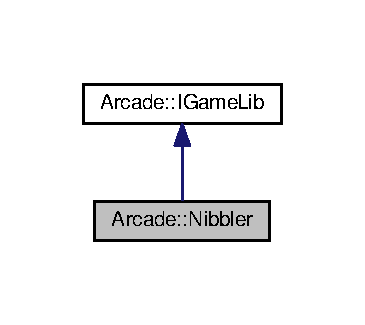
\includegraphics[width=175pt]{class_arcade_1_1_nibbler__inherit__graph}
\end{center}
\end{figure}


Collaboration diagram for Arcade\+:\+:Nibbler\+:
\nopagebreak
\begin{figure}[H]
\begin{center}
\leavevmode
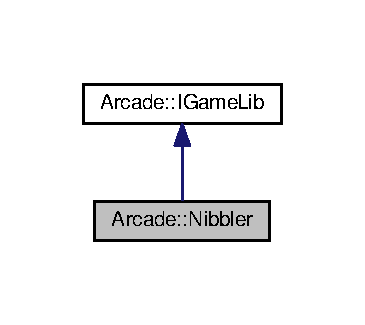
\includegraphics[width=175pt]{class_arcade_1_1_nibbler__coll__graph}
\end{center}
\end{figure}
\subsection*{Public Member Functions}
\begin{DoxyCompactItemize}
\item 
const std\+::string \hyperlink{class_arcade_1_1_nibbler_abbd3cd2246448056bc84b5b893f325d4}{get\+Name} () const final
\begin{DoxyCompactList}\small\item\em Game name\textquotesingle{}s getter. \end{DoxyCompactList}\item 
bool \hyperlink{class_arcade_1_1_nibbler_a244e3c4751d74cab7e4e6ef7b80d0b36}{init} () final
\begin{DoxyCompactList}\small\item\em Init the resources needed by the game to run. \end{DoxyCompactList}\item 
bool \hyperlink{class_arcade_1_1_nibbler_ab88c7e92e23e603b6bd1ccbb6c1ab844}{stop} () final
\begin{DoxyCompactList}\small\item\em Unloads the library. \end{DoxyCompactList}\item 
bool \hyperlink{class_arcade_1_1_nibbler_a979cdf9080be6cb60bf1b4e757029845}{apply\+Event} (\hyperlink{namespace_arcade_a9b501908b20bc993e4f8226db5323c41}{Keys} key) final
\begin{DoxyCompactList}\small\item\em Processes the key obtained by the \hyperlink{class_arcade_1_1_i_graphic_lib}{I\+Graphic\+Lib} from the user to update the game state. \end{DoxyCompactList}\item 
bool \hyperlink{class_arcade_1_1_nibbler_a13199140bc927065b1c59ae2c70e06cf}{update} () final
\begin{DoxyCompactList}\small\item\em Updates the game state. \end{DoxyCompactList}\item 
void \hyperlink{class_arcade_1_1_nibbler_a69a64ec51964772a03cf7d4bb9088b5b}{refresh} (\hyperlink{class_arcade_1_1_i_graphic_lib}{I\+Graphic\+Lib} \&graphic\+Lib) final
\item 
size\+\_\+t \hyperlink{class_arcade_1_1_nibbler_a861f3bebe3b7f5efe1f3a46eb71957bb}{get\+Score} () final
\begin{DoxyCompactList}\small\item\em Current player score\textquotesingle{}s getter. \end{DoxyCompactList}\end{DoxyCompactItemize}


\subsection{Member Function Documentation}
\mbox{\Hypertarget{class_arcade_1_1_nibbler_a979cdf9080be6cb60bf1b4e757029845}\label{class_arcade_1_1_nibbler_a979cdf9080be6cb60bf1b4e757029845}} 
\index{Arcade\+::\+Nibbler@{Arcade\+::\+Nibbler}!apply\+Event@{apply\+Event}}
\index{apply\+Event@{apply\+Event}!Arcade\+::\+Nibbler@{Arcade\+::\+Nibbler}}
\subsubsection{\texorpdfstring{apply\+Event()}{applyEvent()}}
{\footnotesize\ttfamily bool Arcade\+::\+Nibbler\+::apply\+Event (\begin{DoxyParamCaption}\item[{\hyperlink{namespace_arcade_a9b501908b20bc993e4f8226db5323c41}{Keys}}]{key }\end{DoxyParamCaption})\hspace{0.3cm}{\ttfamily [final]}, {\ttfamily [virtual]}}



Processes the key obtained by the \hyperlink{class_arcade_1_1_i_graphic_lib}{I\+Graphic\+Lib} from the user to update the game state. 


\begin{DoxyParams}{Parameters}
{\em key} & \+: enum value of the obtained key \\
\hline
\end{DoxyParams}
\begin{DoxyReturn}{Returns}
true if the game is still in progress, false in case of defeat 
\end{DoxyReturn}


Implements \hyperlink{class_arcade_1_1_i_game_lib_a3b1b66ec00899b4c9efcd6151bf2497e}{Arcade\+::\+I\+Game\+Lib}.

\mbox{\Hypertarget{class_arcade_1_1_nibbler_abbd3cd2246448056bc84b5b893f325d4}\label{class_arcade_1_1_nibbler_abbd3cd2246448056bc84b5b893f325d4}} 
\index{Arcade\+::\+Nibbler@{Arcade\+::\+Nibbler}!get\+Name@{get\+Name}}
\index{get\+Name@{get\+Name}!Arcade\+::\+Nibbler@{Arcade\+::\+Nibbler}}
\subsubsection{\texorpdfstring{get\+Name()}{getName()}}
{\footnotesize\ttfamily const std\+::string Arcade\+::\+Nibbler\+::get\+Name (\begin{DoxyParamCaption}{ }\end{DoxyParamCaption}) const\hspace{0.3cm}{\ttfamily [final]}, {\ttfamily [virtual]}}



Game name\textquotesingle{}s getter. 

\begin{DoxyReturn}{Returns}
a string containing the name of the game 
\end{DoxyReturn}


Implements \hyperlink{class_arcade_1_1_i_game_lib_afd2652d62ebfda4caa5d0c05ff40ed61}{Arcade\+::\+I\+Game\+Lib}.

\mbox{\Hypertarget{class_arcade_1_1_nibbler_a861f3bebe3b7f5efe1f3a46eb71957bb}\label{class_arcade_1_1_nibbler_a861f3bebe3b7f5efe1f3a46eb71957bb}} 
\index{Arcade\+::\+Nibbler@{Arcade\+::\+Nibbler}!get\+Score@{get\+Score}}
\index{get\+Score@{get\+Score}!Arcade\+::\+Nibbler@{Arcade\+::\+Nibbler}}
\subsubsection{\texorpdfstring{get\+Score()}{getScore()}}
{\footnotesize\ttfamily size\+\_\+t Arcade\+::\+Nibbler\+::get\+Score (\begin{DoxyParamCaption}{ }\end{DoxyParamCaption})\hspace{0.3cm}{\ttfamily [final]}, {\ttfamily [virtual]}}



Current player score\textquotesingle{}s getter. 

\begin{DoxyReturn}{Returns}
the player score
\end{DoxyReturn}
To call at the end of the execution of the game (after the player loose or win) for getting his score 

Implements \hyperlink{class_arcade_1_1_i_game_lib_a00cdcad68c670aecbcc249a2995833b6}{Arcade\+::\+I\+Game\+Lib}.

\mbox{\Hypertarget{class_arcade_1_1_nibbler_a244e3c4751d74cab7e4e6ef7b80d0b36}\label{class_arcade_1_1_nibbler_a244e3c4751d74cab7e4e6ef7b80d0b36}} 
\index{Arcade\+::\+Nibbler@{Arcade\+::\+Nibbler}!init@{init}}
\index{init@{init}!Arcade\+::\+Nibbler@{Arcade\+::\+Nibbler}}
\subsubsection{\texorpdfstring{init()}{init()}}
{\footnotesize\ttfamily bool Arcade\+::\+Nibbler\+::init (\begin{DoxyParamCaption}{ }\end{DoxyParamCaption})\hspace{0.3cm}{\ttfamily [final]}, {\ttfamily [virtual]}}



Init the resources needed by the game to run. 

\begin{DoxyReturn}{Returns}
true if succeed, otherwise returns false 
\end{DoxyReturn}


Implements \hyperlink{class_arcade_1_1_i_game_lib_aacc4169a98dfeb007bcaf9dfeece9e08}{Arcade\+::\+I\+Game\+Lib}.

\mbox{\Hypertarget{class_arcade_1_1_nibbler_a69a64ec51964772a03cf7d4bb9088b5b}\label{class_arcade_1_1_nibbler_a69a64ec51964772a03cf7d4bb9088b5b}} 
\index{Arcade\+::\+Nibbler@{Arcade\+::\+Nibbler}!refresh@{refresh}}
\index{refresh@{refresh}!Arcade\+::\+Nibbler@{Arcade\+::\+Nibbler}}
\subsubsection{\texorpdfstring{refresh()}{refresh()}}
{\footnotesize\ttfamily void Arcade\+::\+Nibbler\+::refresh (\begin{DoxyParamCaption}\item[{\hyperlink{class_arcade_1_1_i_graphic_lib}{I\+Graphic\+Lib} \&}]{graphic\+Lib }\end{DoxyParamCaption})\hspace{0.3cm}{\ttfamily [final]}, {\ttfamily [virtual]}}

Renders the game state to the screen. 
\begin{DoxyParams}{Parameters}
{\em graphic\+Lib} & \+: Loaded graphics library used for rendering.\\
\hline
\end{DoxyParams}
This should call I\+Graphic\+Lib\+::refresh() to display content to the user. 

Implements \hyperlink{class_arcade_1_1_i_game_lib_a00c3d335ef313e441217b33dcf7844df}{Arcade\+::\+I\+Game\+Lib}.

\mbox{\Hypertarget{class_arcade_1_1_nibbler_ab88c7e92e23e603b6bd1ccbb6c1ab844}\label{class_arcade_1_1_nibbler_ab88c7e92e23e603b6bd1ccbb6c1ab844}} 
\index{Arcade\+::\+Nibbler@{Arcade\+::\+Nibbler}!stop@{stop}}
\index{stop@{stop}!Arcade\+::\+Nibbler@{Arcade\+::\+Nibbler}}
\subsubsection{\texorpdfstring{stop()}{stop()}}
{\footnotesize\ttfamily bool Arcade\+::\+Nibbler\+::stop (\begin{DoxyParamCaption}{ }\end{DoxyParamCaption})\hspace{0.3cm}{\ttfamily [final]}, {\ttfamily [virtual]}}



Unloads the library. 

\begin{DoxyReturn}{Returns}
true if succeed, otherwise returns false 
\end{DoxyReturn}


Implements \hyperlink{class_arcade_1_1_i_game_lib_ab9b7c1bbbea1b86e8515e8fd188fe9cb}{Arcade\+::\+I\+Game\+Lib}.

\mbox{\Hypertarget{class_arcade_1_1_nibbler_a13199140bc927065b1c59ae2c70e06cf}\label{class_arcade_1_1_nibbler_a13199140bc927065b1c59ae2c70e06cf}} 
\index{Arcade\+::\+Nibbler@{Arcade\+::\+Nibbler}!update@{update}}
\index{update@{update}!Arcade\+::\+Nibbler@{Arcade\+::\+Nibbler}}
\subsubsection{\texorpdfstring{update()}{update()}}
{\footnotesize\ttfamily bool Arcade\+::\+Nibbler\+::update (\begin{DoxyParamCaption}{ }\end{DoxyParamCaption})\hspace{0.3cm}{\ttfamily [final]}, {\ttfamily [virtual]}}



Updates the game state. 

\begin{DoxyReturn}{Returns}
true if the game is still in progress, false in case of defeat
\end{DoxyReturn}
Move the player forward and/or move the N\+P\+Cs, according to the game\textquotesingle{}s rules 

Implements \hyperlink{class_arcade_1_1_i_game_lib_a0be7ffaa269e2fa47146bf27ad2c511a}{Arcade\+::\+I\+Game\+Lib}.



The documentation for this class was generated from the following files\+:\begin{DoxyCompactItemize}
\item 
/home/rectoria/projects/epitech/\+C\+P\+P/cpp\+\_\+arcade/games/nibbler/Nibbler.\+hpp\item 
/home/rectoria/projects/epitech/\+C\+P\+P/cpp\+\_\+arcade/games/nibbler/Nibbler.\+cpp\end{DoxyCompactItemize}

\hypertarget{class_arcade_1_1_pacman}{}\section{Arcade\+:\+:Pacman Class Reference}
\label{class_arcade_1_1_pacman}\index{Arcade\+::\+Pacman@{Arcade\+::\+Pacman}}


Inheritance diagram for Arcade\+:\+:Pacman\+:
\nopagebreak
\begin{figure}[H]
\begin{center}
\leavevmode
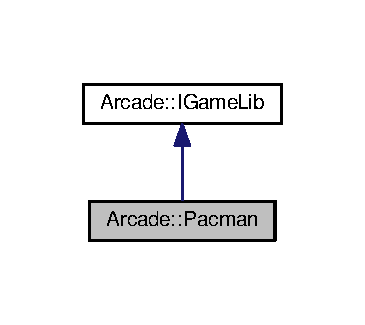
\includegraphics[width=175pt]{class_arcade_1_1_pacman__inherit__graph}
\end{center}
\end{figure}


Collaboration diagram for Arcade\+:\+:Pacman\+:
\nopagebreak
\begin{figure}[H]
\begin{center}
\leavevmode
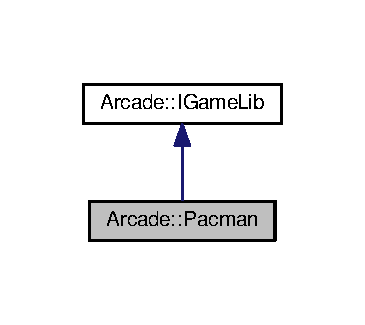
\includegraphics[width=175pt]{class_arcade_1_1_pacman__coll__graph}
\end{center}
\end{figure}
\subsection*{Public Member Functions}
\begin{DoxyCompactItemize}
\item 
const std\+::string \hyperlink{class_arcade_1_1_pacman_abc48d59a534276889f45128fe877d5d9}{get\+Name} () const final
\begin{DoxyCompactList}\small\item\em Game name\textquotesingle{}s getter. \end{DoxyCompactList}\item 
bool \hyperlink{class_arcade_1_1_pacman_a27b0ecc843707c735ed1b65e7da009e1}{init} () final
\begin{DoxyCompactList}\small\item\em Init the resources needed by the game to run. \end{DoxyCompactList}\item 
bool \hyperlink{class_arcade_1_1_pacman_a2787800feab139ddeabb11d6ee23a80e}{stop} () final
\begin{DoxyCompactList}\small\item\em Unloads the library. \end{DoxyCompactList}\item 
bool \hyperlink{class_arcade_1_1_pacman_ac5fa3a4d5eaa81d37e8b63451265870d}{apply\+Event} (\hyperlink{namespace_arcade_a9b501908b20bc993e4f8226db5323c41}{Arcade\+::\+Keys}) final
\begin{DoxyCompactList}\small\item\em Processes the key obtained by the \hyperlink{class_arcade_1_1_i_graphic_lib}{I\+Graphic\+Lib} from the user to update the game state. \end{DoxyCompactList}\item 
bool \hyperlink{class_arcade_1_1_pacman_aacb11530e954870a6939d91794cbe356}{update} () final
\begin{DoxyCompactList}\small\item\em Updates the game state. \end{DoxyCompactList}\item 
void \hyperlink{class_arcade_1_1_pacman_ad0d57afab410c98d4050c030b06ad63a}{refresh} (\hyperlink{class_arcade_1_1_i_graphic_lib}{I\+Graphic\+Lib} \&) final
\item 
size\+\_\+t \hyperlink{class_arcade_1_1_pacman_a7683729dd33fb18673c4d77764ca1831}{get\+Score} () final
\begin{DoxyCompactList}\small\item\em Current player score\textquotesingle{}s getter. \end{DoxyCompactList}\end{DoxyCompactItemize}


\subsection{Member Function Documentation}
\mbox{\Hypertarget{class_arcade_1_1_pacman_ac5fa3a4d5eaa81d37e8b63451265870d}\label{class_arcade_1_1_pacman_ac5fa3a4d5eaa81d37e8b63451265870d}} 
\index{Arcade\+::\+Pacman@{Arcade\+::\+Pacman}!apply\+Event@{apply\+Event}}
\index{apply\+Event@{apply\+Event}!Arcade\+::\+Pacman@{Arcade\+::\+Pacman}}
\subsubsection{\texorpdfstring{apply\+Event()}{applyEvent()}}
{\footnotesize\ttfamily bool Arcade\+::\+Pacman\+::apply\+Event (\begin{DoxyParamCaption}\item[{\hyperlink{namespace_arcade_a9b501908b20bc993e4f8226db5323c41}{Arcade\+::\+Keys}}]{key }\end{DoxyParamCaption})\hspace{0.3cm}{\ttfamily [final]}, {\ttfamily [virtual]}}



Processes the key obtained by the \hyperlink{class_arcade_1_1_i_graphic_lib}{I\+Graphic\+Lib} from the user to update the game state. 


\begin{DoxyParams}{Parameters}
{\em key} & \+: enum value of the obtained key \\
\hline
\end{DoxyParams}
\begin{DoxyReturn}{Returns}
true if the game is still in progress, false in case of defeat 
\end{DoxyReturn}


Implements \hyperlink{class_arcade_1_1_i_game_lib_a3b1b66ec00899b4c9efcd6151bf2497e}{Arcade\+::\+I\+Game\+Lib}.

\mbox{\Hypertarget{class_arcade_1_1_pacman_abc48d59a534276889f45128fe877d5d9}\label{class_arcade_1_1_pacman_abc48d59a534276889f45128fe877d5d9}} 
\index{Arcade\+::\+Pacman@{Arcade\+::\+Pacman}!get\+Name@{get\+Name}}
\index{get\+Name@{get\+Name}!Arcade\+::\+Pacman@{Arcade\+::\+Pacman}}
\subsubsection{\texorpdfstring{get\+Name()}{getName()}}
{\footnotesize\ttfamily const std\+::string Arcade\+::\+Pacman\+::get\+Name (\begin{DoxyParamCaption}{ }\end{DoxyParamCaption}) const\hspace{0.3cm}{\ttfamily [final]}, {\ttfamily [virtual]}}



Game name\textquotesingle{}s getter. 

\begin{DoxyReturn}{Returns}
a string containing the name of the game 
\end{DoxyReturn}


Implements \hyperlink{class_arcade_1_1_i_game_lib_afd2652d62ebfda4caa5d0c05ff40ed61}{Arcade\+::\+I\+Game\+Lib}.

\mbox{\Hypertarget{class_arcade_1_1_pacman_a7683729dd33fb18673c4d77764ca1831}\label{class_arcade_1_1_pacman_a7683729dd33fb18673c4d77764ca1831}} 
\index{Arcade\+::\+Pacman@{Arcade\+::\+Pacman}!get\+Score@{get\+Score}}
\index{get\+Score@{get\+Score}!Arcade\+::\+Pacman@{Arcade\+::\+Pacman}}
\subsubsection{\texorpdfstring{get\+Score()}{getScore()}}
{\footnotesize\ttfamily size\+\_\+t Arcade\+::\+Pacman\+::get\+Score (\begin{DoxyParamCaption}{ }\end{DoxyParamCaption})\hspace{0.3cm}{\ttfamily [final]}, {\ttfamily [virtual]}}



Current player score\textquotesingle{}s getter. 

\begin{DoxyReturn}{Returns}
the player score
\end{DoxyReturn}
To call at the end of the execution of the game (after the player loose or win) for getting his score 

Implements \hyperlink{class_arcade_1_1_i_game_lib_a00cdcad68c670aecbcc249a2995833b6}{Arcade\+::\+I\+Game\+Lib}.

\mbox{\Hypertarget{class_arcade_1_1_pacman_a27b0ecc843707c735ed1b65e7da009e1}\label{class_arcade_1_1_pacman_a27b0ecc843707c735ed1b65e7da009e1}} 
\index{Arcade\+::\+Pacman@{Arcade\+::\+Pacman}!init@{init}}
\index{init@{init}!Arcade\+::\+Pacman@{Arcade\+::\+Pacman}}
\subsubsection{\texorpdfstring{init()}{init()}}
{\footnotesize\ttfamily bool Arcade\+::\+Pacman\+::init (\begin{DoxyParamCaption}{ }\end{DoxyParamCaption})\hspace{0.3cm}{\ttfamily [final]}, {\ttfamily [virtual]}}



Init the resources needed by the game to run. 

\begin{DoxyReturn}{Returns}
true if succeed, otherwise returns false 
\end{DoxyReturn}


Implements \hyperlink{class_arcade_1_1_i_game_lib_aacc4169a98dfeb007bcaf9dfeece9e08}{Arcade\+::\+I\+Game\+Lib}.

\mbox{\Hypertarget{class_arcade_1_1_pacman_ad0d57afab410c98d4050c030b06ad63a}\label{class_arcade_1_1_pacman_ad0d57afab410c98d4050c030b06ad63a}} 
\index{Arcade\+::\+Pacman@{Arcade\+::\+Pacman}!refresh@{refresh}}
\index{refresh@{refresh}!Arcade\+::\+Pacman@{Arcade\+::\+Pacman}}
\subsubsection{\texorpdfstring{refresh()}{refresh()}}
{\footnotesize\ttfamily void Arcade\+::\+Pacman\+::refresh (\begin{DoxyParamCaption}\item[{\hyperlink{class_arcade_1_1_i_graphic_lib}{I\+Graphic\+Lib} \&}]{graphic\+Lib }\end{DoxyParamCaption})\hspace{0.3cm}{\ttfamily [final]}, {\ttfamily [virtual]}}

Renders the game state to the screen. 
\begin{DoxyParams}{Parameters}
{\em graphic\+Lib} & \+: Loaded graphics library used for rendering.\\
\hline
\end{DoxyParams}
This should call I\+Graphic\+Lib\+::refresh() to display content to the user. 

Implements \hyperlink{class_arcade_1_1_i_game_lib_a00c3d335ef313e441217b33dcf7844df}{Arcade\+::\+I\+Game\+Lib}.

\mbox{\Hypertarget{class_arcade_1_1_pacman_a2787800feab139ddeabb11d6ee23a80e}\label{class_arcade_1_1_pacman_a2787800feab139ddeabb11d6ee23a80e}} 
\index{Arcade\+::\+Pacman@{Arcade\+::\+Pacman}!stop@{stop}}
\index{stop@{stop}!Arcade\+::\+Pacman@{Arcade\+::\+Pacman}}
\subsubsection{\texorpdfstring{stop()}{stop()}}
{\footnotesize\ttfamily bool Arcade\+::\+Pacman\+::stop (\begin{DoxyParamCaption}{ }\end{DoxyParamCaption})\hspace{0.3cm}{\ttfamily [final]}, {\ttfamily [virtual]}}



Unloads the library. 

\begin{DoxyReturn}{Returns}
true if succeed, otherwise returns false 
\end{DoxyReturn}


Implements \hyperlink{class_arcade_1_1_i_game_lib_ab9b7c1bbbea1b86e8515e8fd188fe9cb}{Arcade\+::\+I\+Game\+Lib}.

\mbox{\Hypertarget{class_arcade_1_1_pacman_aacb11530e954870a6939d91794cbe356}\label{class_arcade_1_1_pacman_aacb11530e954870a6939d91794cbe356}} 
\index{Arcade\+::\+Pacman@{Arcade\+::\+Pacman}!update@{update}}
\index{update@{update}!Arcade\+::\+Pacman@{Arcade\+::\+Pacman}}
\subsubsection{\texorpdfstring{update()}{update()}}
{\footnotesize\ttfamily bool Arcade\+::\+Pacman\+::update (\begin{DoxyParamCaption}{ }\end{DoxyParamCaption})\hspace{0.3cm}{\ttfamily [final]}, {\ttfamily [virtual]}}



Updates the game state. 

\begin{DoxyReturn}{Returns}
true if the game is still in progress, false in case of defeat
\end{DoxyReturn}
Move the player forward and/or move the N\+P\+Cs, according to the game\textquotesingle{}s rules 

Implements \hyperlink{class_arcade_1_1_i_game_lib_a0be7ffaa269e2fa47146bf27ad2c511a}{Arcade\+::\+I\+Game\+Lib}.



The documentation for this class was generated from the following files\+:\begin{DoxyCompactItemize}
\item 
/home/rectoria/projects/epitech/\+C\+P\+P/cpp\+\_\+arcade/games/pacman/Pacman.\+hpp\item 
/home/rectoria/projects/epitech/\+C\+P\+P/cpp\+\_\+arcade/games/pacman/Pacman.\+cpp\end{DoxyCompactItemize}

\hypertarget{class_arcade_1_1_pixel_box}{}\section{Arcade\+:\+:Pixel\+Box Class Reference}
\label{class_arcade_1_1_pixel_box}\index{Arcade\+::\+Pixel\+Box@{Arcade\+::\+Pixel\+Box}}


\hyperlink{class_arcade_1_1_pixel_box}{Pixel\+Box} class.  




{\ttfamily \#include $<$Pixel\+Box.\+hpp$>$}

\subsection*{Public Member Functions}
\begin{DoxyCompactItemize}
\item 
\hyperlink{class_arcade_1_1_pixel_box_adec96dbc5af889192e59ace1330f573e}{Pixel\+Box} (\hyperlink{class_arcade_1_1_vect}{Vect}$<$ size\+\_\+t $>$ size=\hyperlink{class_arcade_1_1_vect}{Vect}$<$ size\+\_\+t $>$(), \hyperlink{class_arcade_1_1_vect}{Vect}$<$ size\+\_\+t $>$ pos=\hyperlink{class_arcade_1_1_vect}{Vect}$<$ size\+\_\+t $>$(), \hyperlink{class_arcade_1_1_color}{Color} col=\hyperlink{class_arcade_1_1_color}{Color}(255, 255, 255, 255))
\begin{DoxyCompactList}\small\item\em \hyperlink{class_arcade_1_1_pixel_box}{Pixel\+Box} class\textquotesingle{}s constructor. \end{DoxyCompactList}\item 
\mbox{\Hypertarget{class_arcade_1_1_pixel_box_a3172153d8141b2d9812631444f8d9a85}\label{class_arcade_1_1_pixel_box_a3172153d8141b2d9812631444f8d9a85}} 
\hyperlink{class_arcade_1_1_pixel_box_a3172153d8141b2d9812631444f8d9a85}{$\sim$\+Pixel\+Box} ()=default
\begin{DoxyCompactList}\small\item\em \hyperlink{class_arcade_1_1_pixel_box}{Pixel\+Box} class\textquotesingle{}s destructor. \end{DoxyCompactList}\item 
size\+\_\+t \hyperlink{class_arcade_1_1_pixel_box_ad9d260f2ab0c0951aad39d9773e6660f}{get\+Height} () const
\begin{DoxyCompactList}\small\item\em \hyperlink{class_arcade_1_1_pixel_box}{Pixel\+Box} height\textquotesingle{}s getter. \end{DoxyCompactList}\item 
size\+\_\+t \hyperlink{class_arcade_1_1_pixel_box_a67b98640d591223f1e898d8d8158ab48}{getY} () const
\begin{DoxyCompactList}\small\item\em \hyperlink{class_arcade_1_1_pixel_box}{Pixel\+Box} Y offset\textquotesingle{}s getter. \end{DoxyCompactList}\item 
\mbox{\Hypertarget{class_arcade_1_1_pixel_box_a5891000ec0f34dc353605a22fc967d44}\label{class_arcade_1_1_pixel_box_a5891000ec0f34dc353605a22fc967d44}} 
void \hyperlink{class_arcade_1_1_pixel_box_a5891000ec0f34dc353605a22fc967d44}{set\+Height} (size\+\_\+t height)
\begin{DoxyCompactList}\small\item\em \hyperlink{class_arcade_1_1_pixel_box}{Pixel\+Box} height setter. \end{DoxyCompactList}\item 
\mbox{\Hypertarget{class_arcade_1_1_pixel_box_a07686b40c6979af70a8eb8ac02940116}\label{class_arcade_1_1_pixel_box_a07686b40c6979af70a8eb8ac02940116}} 
void \hyperlink{class_arcade_1_1_pixel_box_a07686b40c6979af70a8eb8ac02940116}{setY} (size\+\_\+t y)
\begin{DoxyCompactList}\small\item\em \hyperlink{class_arcade_1_1_pixel_box}{Pixel\+Box} Y offset\textquotesingle{}s getter. \end{DoxyCompactList}\item 
size\+\_\+t \hyperlink{class_arcade_1_1_pixel_box_a004ea9244a8ebc163c1e3fa06bdf8c4a}{get\+Width} () const
\begin{DoxyCompactList}\small\item\em \hyperlink{class_arcade_1_1_pixel_box}{Pixel\+Box} width\textquotesingle{}s getter. \end{DoxyCompactList}\item 
size\+\_\+t \hyperlink{class_arcade_1_1_pixel_box_a17c96dac5f262348f15627705fdb1db6}{getX} () const
\begin{DoxyCompactList}\small\item\em \hyperlink{class_arcade_1_1_pixel_box}{Pixel\+Box} X offset\textquotesingle{}s getter. \end{DoxyCompactList}\item 
\mbox{\Hypertarget{class_arcade_1_1_pixel_box_acd8daded11a3a7d704821afeafb918d3}\label{class_arcade_1_1_pixel_box_acd8daded11a3a7d704821afeafb918d3}} 
void \hyperlink{class_arcade_1_1_pixel_box_acd8daded11a3a7d704821afeafb918d3}{set\+Width} (size\+\_\+t width)
\begin{DoxyCompactList}\small\item\em \hyperlink{class_arcade_1_1_pixel_box}{Pixel\+Box} height\textquotesingle{}s setter. \end{DoxyCompactList}\item 
\mbox{\Hypertarget{class_arcade_1_1_pixel_box_a6c184f4d988c76cabe7bd50be6e8f667}\label{class_arcade_1_1_pixel_box_a6c184f4d988c76cabe7bd50be6e8f667}} 
void \hyperlink{class_arcade_1_1_pixel_box_a6c184f4d988c76cabe7bd50be6e8f667}{setX} (size\+\_\+t x)
\begin{DoxyCompactList}\small\item\em \hyperlink{class_arcade_1_1_pixel_box}{Pixel\+Box} X offset\textquotesingle{}s setter. \end{DoxyCompactList}\item 
\hyperlink{class_arcade_1_1_vect}{Vect}$<$ size\+\_\+t $>$ \hyperlink{class_arcade_1_1_pixel_box_a8f0280a28955151ee0662b206779d06d}{get\+Size} () const
\begin{DoxyCompactList}\small\item\em \hyperlink{class_arcade_1_1_pixel_box}{Pixel\+Box} dimensions\textquotesingle{}s getter. \end{DoxyCompactList}\item 
void \hyperlink{class_arcade_1_1_pixel_box_ad0682049ca567f2a963528d1d5d8c62b}{set\+Size} (\hyperlink{class_arcade_1_1_vect}{Vect}$<$ size\+\_\+t $>$ size)
\begin{DoxyCompactList}\small\item\em \hyperlink{class_arcade_1_1_pixel_box}{Pixel\+Box} dimensions\textquotesingle{}s getter. \end{DoxyCompactList}\item 
\hyperlink{class_arcade_1_1_vect}{Vect}$<$ size\+\_\+t $>$ \hyperlink{class_arcade_1_1_pixel_box_af041604dd9b7b39a82671b00e445ee0e}{get\+Pos} () const
\begin{DoxyCompactList}\small\item\em \hyperlink{class_arcade_1_1_pixel_box}{Pixel\+Box} positions\textquotesingle{}s getter. \end{DoxyCompactList}\item 
void \hyperlink{class_arcade_1_1_pixel_box_aeb1ca87a35942dc55f129d9de480658b}{set\+Pos} (\hyperlink{class_arcade_1_1_vect}{Vect}$<$ size\+\_\+t $>$ pos)
\begin{DoxyCompactList}\small\item\em \hyperlink{class_arcade_1_1_pixel_box}{Pixel\+Box} positions\textquotesingle{}s setter. \end{DoxyCompactList}\item 
void \hyperlink{class_arcade_1_1_pixel_box_a517214a6fd2fc9007aabe0f4a013ca0c}{put\+Pixel} (\hyperlink{class_arcade_1_1_vect}{Vect}$<$ size\+\_\+t $>$ pos, \hyperlink{class_arcade_1_1_color}{Color} col)
\begin{DoxyCompactList}\small\item\em Sets the color of the pixel at the given position. \end{DoxyCompactList}\item 
\hyperlink{class_arcade_1_1_color}{Color} \hyperlink{class_arcade_1_1_pixel_box_afbbc61f220999095290e62a6eb413301}{get\+Pixel} (\hyperlink{class_arcade_1_1_vect}{Vect}$<$ size\+\_\+t $>$ pos) const
\begin{DoxyCompactList}\small\item\em Getter from pixel color to given position. \end{DoxyCompactList}\item 
void \hyperlink{class_arcade_1_1_pixel_box_ac93dc2a0d6f36f11bf798aafac8968f0}{put\+Rect} (\hyperlink{class_arcade_1_1_vect}{Vect}$<$ size\+\_\+t $>$ pos, \hyperlink{class_arcade_1_1_vect}{Vect}$<$ size\+\_\+t $>$ size, \hyperlink{class_arcade_1_1_color}{Color} col)
\begin{DoxyCompactList}\small\item\em Sets the color of many pixels within the pixel\+Box pixels\textquotesingle{}s array. \end{DoxyCompactList}\item 
std\+::vector$<$ \hyperlink{class_arcade_1_1_color}{Color} $>$ const  \& \hyperlink{class_arcade_1_1_pixel_box_a85ebca9e42c237f806d00d510b504001}{get\+Pixel\+Array} () const
\begin{DoxyCompactList}\small\item\em Getter of the pixels array. \end{DoxyCompactList}\end{DoxyCompactItemize}


\subsection{Detailed Description}
\hyperlink{class_arcade_1_1_pixel_box}{Pixel\+Box} class. 

Class used to represent a rectangle of pixels 

\subsection{Constructor \& Destructor Documentation}
\mbox{\Hypertarget{class_arcade_1_1_pixel_box_adec96dbc5af889192e59ace1330f573e}\label{class_arcade_1_1_pixel_box_adec96dbc5af889192e59ace1330f573e}} 
\index{Arcade\+::\+Pixel\+Box@{Arcade\+::\+Pixel\+Box}!Pixel\+Box@{Pixel\+Box}}
\index{Pixel\+Box@{Pixel\+Box}!Arcade\+::\+Pixel\+Box@{Arcade\+::\+Pixel\+Box}}
\subsubsection{\texorpdfstring{Pixel\+Box()}{PixelBox()}}
{\footnotesize\ttfamily Arcade\+::\+Pixel\+Box\+::\+Pixel\+Box (\begin{DoxyParamCaption}\item[{\hyperlink{class_arcade_1_1_vect}{Arcade\+::\+Vect}$<$ size\+\_\+t $>$}]{size = {\ttfamily \hyperlink{class_arcade_1_1_vect}{Vect}$<$size\+\_\+t$>$()},  }\item[{\hyperlink{class_arcade_1_1_vect}{Arcade\+::\+Vect}$<$ size\+\_\+t $>$}]{pos = {\ttfamily \hyperlink{class_arcade_1_1_vect}{Vect}$<$size\+\_\+t$>$()},  }\item[{\hyperlink{class_arcade_1_1_color}{Arcade\+::\+Color}}]{col = {\ttfamily \hyperlink{class_arcade_1_1_color}{Color}(255,~255,~255,~255)} }\end{DoxyParamCaption})\hspace{0.3cm}{\ttfamily [explicit]}}



\hyperlink{class_arcade_1_1_pixel_box}{Pixel\+Box} class\textquotesingle{}s constructor. 


\begin{DoxyParams}{Parameters}
{\em size} & \+: \hyperlink{class_arcade_1_1_vect}{Vect$<$size\+\_\+t$>$} containing the width (x) and the height (y) of the pixel\+Box \\
\hline
{\em pos} & \+: \hyperlink{class_arcade_1_1_vect}{Vect$<$size\+\_\+t$>$} containing both x and y offsets. Used to place the pixel\+Box on the rendering support \\
\hline
{\em col} & \+: the color with which the array of pixels inside the pixel\+Box will be created\\
\hline
\end{DoxyParams}
Creates a new pixel\+Box class instance. The first \hyperlink{class_arcade_1_1_vect}{Vect$<$size\+\_\+t$>$} size argument defines the dimensions of the pixel\+Box. The second \hyperlink{class_arcade_1_1_vect}{Vect$<$size\+\_\+t$>$} pos argument defines the coordinates of the pixel\+Box\textquotesingle{}s position on the rendering support. It will be the offset applied when rendering it. The third argument defines the color in which the pixels will be created. 

\subsection{Member Function Documentation}
\mbox{\Hypertarget{class_arcade_1_1_pixel_box_ad9d260f2ab0c0951aad39d9773e6660f}\label{class_arcade_1_1_pixel_box_ad9d260f2ab0c0951aad39d9773e6660f}} 
\index{Arcade\+::\+Pixel\+Box@{Arcade\+::\+Pixel\+Box}!get\+Height@{get\+Height}}
\index{get\+Height@{get\+Height}!Arcade\+::\+Pixel\+Box@{Arcade\+::\+Pixel\+Box}}
\subsubsection{\texorpdfstring{get\+Height()}{getHeight()}}
{\footnotesize\ttfamily size\+\_\+t Arcade\+::\+Pixel\+Box\+::get\+Height (\begin{DoxyParamCaption}{ }\end{DoxyParamCaption}) const}



\hyperlink{class_arcade_1_1_pixel_box}{Pixel\+Box} height\textquotesingle{}s getter. 

\begin{DoxyReturn}{Returns}
the pixel\+Box\textquotesingle{}s height 
\end{DoxyReturn}
\mbox{\Hypertarget{class_arcade_1_1_pixel_box_afbbc61f220999095290e62a6eb413301}\label{class_arcade_1_1_pixel_box_afbbc61f220999095290e62a6eb413301}} 
\index{Arcade\+::\+Pixel\+Box@{Arcade\+::\+Pixel\+Box}!get\+Pixel@{get\+Pixel}}
\index{get\+Pixel@{get\+Pixel}!Arcade\+::\+Pixel\+Box@{Arcade\+::\+Pixel\+Box}}
\subsubsection{\texorpdfstring{get\+Pixel()}{getPixel()}}
{\footnotesize\ttfamily \hyperlink{class_arcade_1_1_color}{Arcade\+::\+Color} Arcade\+::\+Pixel\+Box\+::get\+Pixel (\begin{DoxyParamCaption}\item[{\hyperlink{class_arcade_1_1_vect}{Arcade\+::\+Vect}$<$ size\+\_\+t $>$}]{pos }\end{DoxyParamCaption}) const}



Getter from pixel color to given position. 


\begin{DoxyParams}{Parameters}
{\em pos} & \+: The position of the pixel from which the color is requested \\
\hline
\end{DoxyParams}
\begin{DoxyReturn}{Returns}
the color of the requested pixel 
\end{DoxyReturn}
\mbox{\Hypertarget{class_arcade_1_1_pixel_box_a85ebca9e42c237f806d00d510b504001}\label{class_arcade_1_1_pixel_box_a85ebca9e42c237f806d00d510b504001}} 
\index{Arcade\+::\+Pixel\+Box@{Arcade\+::\+Pixel\+Box}!get\+Pixel\+Array@{get\+Pixel\+Array}}
\index{get\+Pixel\+Array@{get\+Pixel\+Array}!Arcade\+::\+Pixel\+Box@{Arcade\+::\+Pixel\+Box}}
\subsubsection{\texorpdfstring{get\+Pixel\+Array()}{getPixelArray()}}
{\footnotesize\ttfamily std\+::vector$<$ \hyperlink{class_arcade_1_1_color}{Arcade\+::\+Color} $>$ const  \& Arcade\+::\+Pixel\+Box\+::get\+Pixel\+Array (\begin{DoxyParamCaption}{ }\end{DoxyParamCaption}) const}



Getter of the pixels array. 

\begin{DoxyReturn}{Returns}
a vector of all the pixels of the pixel\+Box. 
\end{DoxyReturn}
\mbox{\Hypertarget{class_arcade_1_1_pixel_box_af041604dd9b7b39a82671b00e445ee0e}\label{class_arcade_1_1_pixel_box_af041604dd9b7b39a82671b00e445ee0e}} 
\index{Arcade\+::\+Pixel\+Box@{Arcade\+::\+Pixel\+Box}!get\+Pos@{get\+Pos}}
\index{get\+Pos@{get\+Pos}!Arcade\+::\+Pixel\+Box@{Arcade\+::\+Pixel\+Box}}
\subsubsection{\texorpdfstring{get\+Pos()}{getPos()}}
{\footnotesize\ttfamily \hyperlink{class_arcade_1_1_vect}{Arcade\+::\+Vect}$<$ size\+\_\+t $>$ Arcade\+::\+Pixel\+Box\+::get\+Pos (\begin{DoxyParamCaption}{ }\end{DoxyParamCaption}) const}



\hyperlink{class_arcade_1_1_pixel_box}{Pixel\+Box} positions\textquotesingle{}s getter. 

\begin{DoxyReturn}{Returns}
a \hyperlink{class_arcade_1_1_vect}{Vect$<$size\+\_\+t$>$} containing the offsetX (x) and the offsetY (y) of the pixel\+Box. 
\end{DoxyReturn}
\mbox{\Hypertarget{class_arcade_1_1_pixel_box_a8f0280a28955151ee0662b206779d06d}\label{class_arcade_1_1_pixel_box_a8f0280a28955151ee0662b206779d06d}} 
\index{Arcade\+::\+Pixel\+Box@{Arcade\+::\+Pixel\+Box}!get\+Size@{get\+Size}}
\index{get\+Size@{get\+Size}!Arcade\+::\+Pixel\+Box@{Arcade\+::\+Pixel\+Box}}
\subsubsection{\texorpdfstring{get\+Size()}{getSize()}}
{\footnotesize\ttfamily \hyperlink{class_arcade_1_1_vect}{Arcade\+::\+Vect}$<$ size\+\_\+t $>$ Arcade\+::\+Pixel\+Box\+::get\+Size (\begin{DoxyParamCaption}{ }\end{DoxyParamCaption}) const}



\hyperlink{class_arcade_1_1_pixel_box}{Pixel\+Box} dimensions\textquotesingle{}s getter. 

\begin{DoxyReturn}{Returns}
a \hyperlink{class_arcade_1_1_vect}{Vect$<$size\+\_\+t$>$} containing the width (x) and the height (y) of the pixel\+Box. 
\end{DoxyReturn}
\mbox{\Hypertarget{class_arcade_1_1_pixel_box_a004ea9244a8ebc163c1e3fa06bdf8c4a}\label{class_arcade_1_1_pixel_box_a004ea9244a8ebc163c1e3fa06bdf8c4a}} 
\index{Arcade\+::\+Pixel\+Box@{Arcade\+::\+Pixel\+Box}!get\+Width@{get\+Width}}
\index{get\+Width@{get\+Width}!Arcade\+::\+Pixel\+Box@{Arcade\+::\+Pixel\+Box}}
\subsubsection{\texorpdfstring{get\+Width()}{getWidth()}}
{\footnotesize\ttfamily size\+\_\+t Arcade\+::\+Pixel\+Box\+::get\+Width (\begin{DoxyParamCaption}{ }\end{DoxyParamCaption}) const}



\hyperlink{class_arcade_1_1_pixel_box}{Pixel\+Box} width\textquotesingle{}s getter. 

\begin{DoxyReturn}{Returns}
the pixel\+Box\textquotesingle{}s height 
\end{DoxyReturn}
\mbox{\Hypertarget{class_arcade_1_1_pixel_box_a17c96dac5f262348f15627705fdb1db6}\label{class_arcade_1_1_pixel_box_a17c96dac5f262348f15627705fdb1db6}} 
\index{Arcade\+::\+Pixel\+Box@{Arcade\+::\+Pixel\+Box}!getX@{getX}}
\index{getX@{getX}!Arcade\+::\+Pixel\+Box@{Arcade\+::\+Pixel\+Box}}
\subsubsection{\texorpdfstring{get\+X()}{getX()}}
{\footnotesize\ttfamily size\+\_\+t Arcade\+::\+Pixel\+Box\+::getX (\begin{DoxyParamCaption}{ }\end{DoxyParamCaption}) const}



\hyperlink{class_arcade_1_1_pixel_box}{Pixel\+Box} X offset\textquotesingle{}s getter. 

\begin{DoxyReturn}{Returns}
the pixel\+Box X\textquotesingle{}s offset 
\end{DoxyReturn}
\mbox{\Hypertarget{class_arcade_1_1_pixel_box_a67b98640d591223f1e898d8d8158ab48}\label{class_arcade_1_1_pixel_box_a67b98640d591223f1e898d8d8158ab48}} 
\index{Arcade\+::\+Pixel\+Box@{Arcade\+::\+Pixel\+Box}!getY@{getY}}
\index{getY@{getY}!Arcade\+::\+Pixel\+Box@{Arcade\+::\+Pixel\+Box}}
\subsubsection{\texorpdfstring{get\+Y()}{getY()}}
{\footnotesize\ttfamily size\+\_\+t Arcade\+::\+Pixel\+Box\+::getY (\begin{DoxyParamCaption}{ }\end{DoxyParamCaption}) const}



\hyperlink{class_arcade_1_1_pixel_box}{Pixel\+Box} Y offset\textquotesingle{}s getter. 

\begin{DoxyReturn}{Returns}
the pixel\+Box Y\textquotesingle{}s offset 
\end{DoxyReturn}
\mbox{\Hypertarget{class_arcade_1_1_pixel_box_a517214a6fd2fc9007aabe0f4a013ca0c}\label{class_arcade_1_1_pixel_box_a517214a6fd2fc9007aabe0f4a013ca0c}} 
\index{Arcade\+::\+Pixel\+Box@{Arcade\+::\+Pixel\+Box}!put\+Pixel@{put\+Pixel}}
\index{put\+Pixel@{put\+Pixel}!Arcade\+::\+Pixel\+Box@{Arcade\+::\+Pixel\+Box}}
\subsubsection{\texorpdfstring{put\+Pixel()}{putPixel()}}
{\footnotesize\ttfamily void Arcade\+::\+Pixel\+Box\+::put\+Pixel (\begin{DoxyParamCaption}\item[{\hyperlink{class_arcade_1_1_vect}{Arcade\+::\+Vect}$<$ size\+\_\+t $>$}]{pos,  }\item[{\hyperlink{class_arcade_1_1_color}{Arcade\+::\+Color}}]{col }\end{DoxyParamCaption})}



Sets the color of the pixel at the given position. 


\begin{DoxyParams}{Parameters}
{\em pos} & \+: The position of the pixel to be modified \\
\hline
{\em col} & \+: The new color of the pixel to be modified \\
\hline
\end{DoxyParams}
\mbox{\Hypertarget{class_arcade_1_1_pixel_box_ac93dc2a0d6f36f11bf798aafac8968f0}\label{class_arcade_1_1_pixel_box_ac93dc2a0d6f36f11bf798aafac8968f0}} 
\index{Arcade\+::\+Pixel\+Box@{Arcade\+::\+Pixel\+Box}!put\+Rect@{put\+Rect}}
\index{put\+Rect@{put\+Rect}!Arcade\+::\+Pixel\+Box@{Arcade\+::\+Pixel\+Box}}
\subsubsection{\texorpdfstring{put\+Rect()}{putRect()}}
{\footnotesize\ttfamily void Arcade\+::\+Pixel\+Box\+::put\+Rect (\begin{DoxyParamCaption}\item[{\hyperlink{class_arcade_1_1_vect}{Arcade\+::\+Vect}$<$ size\+\_\+t $>$}]{pos,  }\item[{\hyperlink{class_arcade_1_1_vect}{Arcade\+::\+Vect}$<$ size\+\_\+t $>$}]{size,  }\item[{\hyperlink{class_arcade_1_1_color}{Arcade\+::\+Color}}]{col }\end{DoxyParamCaption})}



Sets the color of many pixels within the pixel\+Box pixels\textquotesingle{}s array. 


\begin{DoxyParams}{Parameters}
{\em pos} & \+: The position from which the new color has to be applied \\
\hline
{\em size} & \+: The dimensions of the chunk of pixels to be modified \\
\hline
{\em col} & \+: The new color to apply \\
\hline
\end{DoxyParams}
\mbox{\Hypertarget{class_arcade_1_1_pixel_box_aeb1ca87a35942dc55f129d9de480658b}\label{class_arcade_1_1_pixel_box_aeb1ca87a35942dc55f129d9de480658b}} 
\index{Arcade\+::\+Pixel\+Box@{Arcade\+::\+Pixel\+Box}!set\+Pos@{set\+Pos}}
\index{set\+Pos@{set\+Pos}!Arcade\+::\+Pixel\+Box@{Arcade\+::\+Pixel\+Box}}
\subsubsection{\texorpdfstring{set\+Pos()}{setPos()}}
{\footnotesize\ttfamily void Arcade\+::\+Pixel\+Box\+::set\+Pos (\begin{DoxyParamCaption}\item[{\hyperlink{class_arcade_1_1_vect}{Arcade\+::\+Vect}$<$ size\+\_\+t $>$}]{pos }\end{DoxyParamCaption})}



\hyperlink{class_arcade_1_1_pixel_box}{Pixel\+Box} positions\textquotesingle{}s setter. 


\begin{DoxyParams}{Parameters}
{\em pos} & \+: new positions of the pixel\+Box pixels\textquotesingle{}s array\\
\hline
\end{DoxyParams}
Takes both new positions as parameter, within a \hyperlink{class_arcade_1_1_vect}{Vect$<$size\+\_\+t$>$} \mbox{\Hypertarget{class_arcade_1_1_pixel_box_ad0682049ca567f2a963528d1d5d8c62b}\label{class_arcade_1_1_pixel_box_ad0682049ca567f2a963528d1d5d8c62b}} 
\index{Arcade\+::\+Pixel\+Box@{Arcade\+::\+Pixel\+Box}!set\+Size@{set\+Size}}
\index{set\+Size@{set\+Size}!Arcade\+::\+Pixel\+Box@{Arcade\+::\+Pixel\+Box}}
\subsubsection{\texorpdfstring{set\+Size()}{setSize()}}
{\footnotesize\ttfamily void Arcade\+::\+Pixel\+Box\+::set\+Size (\begin{DoxyParamCaption}\item[{\hyperlink{class_arcade_1_1_vect}{Arcade\+::\+Vect}$<$ size\+\_\+t $>$}]{size }\end{DoxyParamCaption})}



\hyperlink{class_arcade_1_1_pixel_box}{Pixel\+Box} dimensions\textquotesingle{}s getter. 


\begin{DoxyParams}{Parameters}
{\em size} & \+: new dimensions of the pixel\+Box pixels\textquotesingle{}s array\\
\hline
\end{DoxyParams}
Takes both new dimensions as parameter, within a \hyperlink{class_arcade_1_1_vect}{Vect$<$size\+\_\+t$>$} 

The documentation for this class was generated from the following files\+:\begin{DoxyCompactItemize}
\item 
/home/rectoria/projects/epitech/\+C\+P\+P/cpp\+\_\+arcade/include/\hyperlink{_pixel_box_8hpp}{Pixel\+Box.\+hpp}\item 
/home/rectoria/projects/epitech/\+C\+P\+P/cpp\+\_\+arcade/include/Pixel\+Box.\+cpp\end{DoxyCompactItemize}

\hypertarget{class_arcade_1_1_score}{}\section{Arcade\+:\+:Score Class Reference}
\label{class_arcade_1_1_score}\index{Arcade\+::\+Score@{Arcade\+::\+Score}}
\subsection*{Public Member Functions}
\begin{DoxyCompactItemize}
\item 
\mbox{\Hypertarget{class_arcade_1_1_score_a6eaa1ed7e5f60fecf96f90ad895aa68a}\label{class_arcade_1_1_score_a6eaa1ed7e5f60fecf96f90ad895aa68a}} 
void {\bfseries add\+Game} (std\+::string \&)
\item 
\mbox{\Hypertarget{class_arcade_1_1_score_a7bad9a2617b4c2211d439f5716b94340}\label{class_arcade_1_1_score_a7bad9a2617b4c2211d439f5716b94340}} 
std\+::map$<$ std\+::string, std\+::string $>$ {\bfseries get\+Game\+Stats} (std\+::string \&)
\item 
\mbox{\Hypertarget{class_arcade_1_1_score_a9b952d8604c3b1c1bdbda082a27404ab}\label{class_arcade_1_1_score_a9b952d8604c3b1c1bdbda082a27404ab}} 
int {\bfseries get\+Player\+Score} (std\+::string \&, std\+::string \&)
\item 
\mbox{\Hypertarget{class_arcade_1_1_score_ad670e3bf5362c9a8e787b9f7b9ee5922}\label{class_arcade_1_1_score_ad670e3bf5362c9a8e787b9f7b9ee5922}} 
void {\bfseries write\+Stats} (std\+::string)
\item 
\mbox{\Hypertarget{class_arcade_1_1_score_a4588f8bac823b945849c29d42d728f01}\label{class_arcade_1_1_score_a4588f8bac823b945849c29d42d728f01}} 
void {\bfseries set\+Score} (std\+::string \&, std\+::string \&, unsigned)
\end{DoxyCompactItemize}


The documentation for this class was generated from the following files\+:\begin{DoxyCompactItemize}
\item 
/home/rectoria/projects/epitech/\+C\+P\+P/cpp\+\_\+arcade/src/score/Score.\+hpp\item 
/home/rectoria/projects/epitech/\+C\+P\+P/cpp\+\_\+arcade/src/score/Score.\+cpp\end{DoxyCompactItemize}

\hypertarget{class_arcade_1_1_sdl2}{}\section{Arcade\+:\+:Sdl2 Class Reference}
\label{class_arcade_1_1_sdl2}\index{Arcade\+::\+Sdl2@{Arcade\+::\+Sdl2}}


Inheritance diagram for Arcade\+:\+:Sdl2\+:
\nopagebreak
\begin{figure}[H]
\begin{center}
\leavevmode
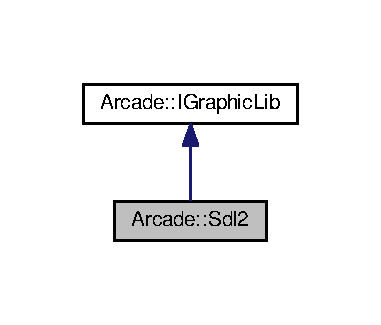
\includegraphics[width=183pt]{class_arcade_1_1_sdl2__inherit__graph}
\end{center}
\end{figure}


Collaboration diagram for Arcade\+:\+:Sdl2\+:
\nopagebreak
\begin{figure}[H]
\begin{center}
\leavevmode
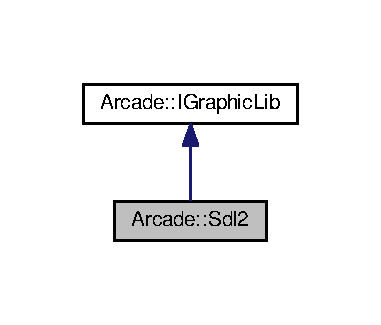
\includegraphics[width=183pt]{class_arcade_1_1_sdl2__coll__graph}
\end{center}
\end{figure}
\subsection*{Public Member Functions}
\begin{DoxyCompactItemize}
\item 
std\+::string \hyperlink{class_arcade_1_1_sdl2_aa1d9e278616747b87d868fadb0272d43}{get\+Name} () const final
\begin{DoxyCompactList}\small\item\em Graphic library name\textquotesingle{}s getter. \end{DoxyCompactList}\item 
bool \hyperlink{class_arcade_1_1_sdl2_a44772ea99509adde0a1c8779265ce260}{is\+Open} () const final
\begin{DoxyCompactList}\small\item\em Specifies whether the window is open or not. \end{DoxyCompactList}\item 
void \hyperlink{class_arcade_1_1_sdl2_a312397e628bbf14d8532e2a13575c7ab}{close\+Renderer} () final
\begin{DoxyCompactList}\small\item\em Closes the rendering support. \end{DoxyCompactList}\item 
void \hyperlink{class_arcade_1_1_sdl2_aa7000a687e79acf5e5ff99ae6e71194b}{open\+Renderer} (std\+::string const \&title) final
\begin{DoxyCompactList}\small\item\em Opens the rendering support. \end{DoxyCompactList}\item 
\mbox{\Hypertarget{class_arcade_1_1_sdl2_a17016501be6ba1d312df65ec65e69fe0}\label{class_arcade_1_1_sdl2_a17016501be6ba1d312df65ec65e69fe0}} 
void \hyperlink{class_arcade_1_1_sdl2_a17016501be6ba1d312df65ec65e69fe0}{clear\+Window} () final
\begin{DoxyCompactList}\small\item\em Clears the rendering support. \end{DoxyCompactList}\item 
\mbox{\Hypertarget{class_arcade_1_1_sdl2_a1bccd13ed46ce1a03003a2c022960968}\label{class_arcade_1_1_sdl2_a1bccd13ed46ce1a03003a2c022960968}} 
void \hyperlink{class_arcade_1_1_sdl2_a1bccd13ed46ce1a03003a2c022960968}{refresh\+Window} () final
\begin{DoxyCompactList}\small\item\em Displays the buffered frame to the screen. \end{DoxyCompactList}\item 
\mbox{\Hypertarget{class_arcade_1_1_sdl2_a8ac8677347067a814e0a4618c815561a}\label{class_arcade_1_1_sdl2_a8ac8677347067a814e0a4618c815561a}} 
void \hyperlink{class_arcade_1_1_sdl2_a8ac8677347067a814e0a4618c815561a}{draw\+Pixel\+Box} (\hyperlink{class_arcade_1_1_pixel_box}{Pixel\+Box} const \&) final
\begin{DoxyCompactList}\small\item\em Draws a \hyperlink{class_arcade_1_1_pixel_box}{Pixel\+Box}. \end{DoxyCompactList}\item 
\mbox{\Hypertarget{class_arcade_1_1_sdl2_ab10797b0556755e2af99fa59d5119fcc}\label{class_arcade_1_1_sdl2_ab10797b0556755e2af99fa59d5119fcc}} 
void \hyperlink{class_arcade_1_1_sdl2_ab10797b0556755e2af99fa59d5119fcc}{draw\+Text} (\hyperlink{class_arcade_1_1_text_box}{Text\+Box} const \&) final
\begin{DoxyCompactList}\small\item\em Draws a \hyperlink{class_arcade_1_1_text_box}{Text\+Box}. \end{DoxyCompactList}\item 
bool \hyperlink{class_arcade_1_1_sdl2_af794699db9401d1be49566908ec7bced}{poll\+Events} () final
\begin{DoxyCompactList}\small\item\em Fetches the events from the user and saves it. \end{DoxyCompactList}\item 
\hyperlink{namespace_arcade_a9b501908b20bc993e4f8226db5323c41}{Keys} \hyperlink{class_arcade_1_1_sdl2_a6d5bda09e7705c6ccef7451694621247}{get\+Last\+Event} () final
\begin{DoxyCompactList}\small\item\em Getter of the oldest command in memory. \end{DoxyCompactList}\item 
void \hyperlink{class_arcade_1_1_sdl2_a92f016d43686b195673aea7f3446d0a1}{clear\+Events} () final
\begin{DoxyCompactList}\small\item\em Clears the pending commands. \end{DoxyCompactList}\item 
\hyperlink{class_arcade_1_1_vect}{Vect}$<$ size\+\_\+t $>$ \hyperlink{class_arcade_1_1_sdl2_ae54d60076b915de4fce36ace576ea01d}{get\+Screen\+Size} () const final
\begin{DoxyCompactList}\small\item\em Getter from the rendering support dimensions. \end{DoxyCompactList}\item 
size\+\_\+t \hyperlink{class_arcade_1_1_sdl2_a958b3611cb0f7db90eeca5c9c4eaed59}{get\+MaxY} () const final
\begin{DoxyCompactList}\small\item\em Getter from the rendering support height. \end{DoxyCompactList}\item 
size\+\_\+t \hyperlink{class_arcade_1_1_sdl2_a9e9e70db8a77c2dee10e2227c70415e3}{get\+MaxX} () const final
\begin{DoxyCompactList}\small\item\em Getter from the rendering support width. \end{DoxyCompactList}\end{DoxyCompactItemize}


\subsection{Member Function Documentation}
\mbox{\Hypertarget{class_arcade_1_1_sdl2_a92f016d43686b195673aea7f3446d0a1}\label{class_arcade_1_1_sdl2_a92f016d43686b195673aea7f3446d0a1}} 
\index{Arcade\+::\+Sdl2@{Arcade\+::\+Sdl2}!clear\+Events@{clear\+Events}}
\index{clear\+Events@{clear\+Events}!Arcade\+::\+Sdl2@{Arcade\+::\+Sdl2}}
\subsubsection{\texorpdfstring{clear\+Events()}{clearEvents()}}
{\footnotesize\ttfamily void Arcade\+::\+Sdl2\+::clear\+Events (\begin{DoxyParamCaption}{ }\end{DoxyParamCaption})\hspace{0.3cm}{\ttfamily [final]}, {\ttfamily [virtual]}}



Clears the pending commands. 

The function deletes all the commands currently stored. They wont be accessible anymore, even with the \hyperlink{class_arcade_1_1_sdl2_a6d5bda09e7705c6ccef7451694621247}{get\+Last\+Event()} method. 

Implements \hyperlink{class_arcade_1_1_i_graphic_lib_a78691f8f9433b2af945576231534c1e3}{Arcade\+::\+I\+Graphic\+Lib}.

\mbox{\Hypertarget{class_arcade_1_1_sdl2_a312397e628bbf14d8532e2a13575c7ab}\label{class_arcade_1_1_sdl2_a312397e628bbf14d8532e2a13575c7ab}} 
\index{Arcade\+::\+Sdl2@{Arcade\+::\+Sdl2}!close\+Renderer@{close\+Renderer}}
\index{close\+Renderer@{close\+Renderer}!Arcade\+::\+Sdl2@{Arcade\+::\+Sdl2}}
\subsubsection{\texorpdfstring{close\+Renderer()}{closeRenderer()}}
{\footnotesize\ttfamily void Arcade\+::\+Sdl2\+::close\+Renderer (\begin{DoxyParamCaption}{ }\end{DoxyParamCaption})\hspace{0.3cm}{\ttfamily [final]}, {\ttfamily [virtual]}}



Closes the rendering support. 

Usually closes a window. Some graphic library uses other rendering support. 

Implements \hyperlink{class_arcade_1_1_i_graphic_lib_aa7c3c8b922fbc94f5e74ecfebad52742}{Arcade\+::\+I\+Graphic\+Lib}.

\mbox{\Hypertarget{class_arcade_1_1_sdl2_a6d5bda09e7705c6ccef7451694621247}\label{class_arcade_1_1_sdl2_a6d5bda09e7705c6ccef7451694621247}} 
\index{Arcade\+::\+Sdl2@{Arcade\+::\+Sdl2}!get\+Last\+Event@{get\+Last\+Event}}
\index{get\+Last\+Event@{get\+Last\+Event}!Arcade\+::\+Sdl2@{Arcade\+::\+Sdl2}}
\subsubsection{\texorpdfstring{get\+Last\+Event()}{getLastEvent()}}
{\footnotesize\ttfamily \hyperlink{namespace_arcade_a9b501908b20bc993e4f8226db5323c41}{Arcade\+::\+Keys} Arcade\+::\+Sdl2\+::get\+Last\+Event (\begin{DoxyParamCaption}{ }\end{DoxyParamCaption})\hspace{0.3cm}{\ttfamily [final]}, {\ttfamily [virtual]}}



Getter of the oldest command in memory. 

\begin{DoxyReturn}{Returns}
the first event of the list.
\end{DoxyReturn}
The function deletes the command if it succeed to retrieves one, using front() and pop\+\_\+front() methods 

Implements \hyperlink{class_arcade_1_1_i_graphic_lib_a801ebd3cff2c861e4b2a1e664c123da7}{Arcade\+::\+I\+Graphic\+Lib}.

\mbox{\Hypertarget{class_arcade_1_1_sdl2_a9e9e70db8a77c2dee10e2227c70415e3}\label{class_arcade_1_1_sdl2_a9e9e70db8a77c2dee10e2227c70415e3}} 
\index{Arcade\+::\+Sdl2@{Arcade\+::\+Sdl2}!get\+MaxX@{get\+MaxX}}
\index{get\+MaxX@{get\+MaxX}!Arcade\+::\+Sdl2@{Arcade\+::\+Sdl2}}
\subsubsection{\texorpdfstring{get\+Max\+X()}{getMaxX()}}
{\footnotesize\ttfamily size\+\_\+t Arcade\+::\+Sdl2\+::get\+MaxX (\begin{DoxyParamCaption}{ }\end{DoxyParamCaption}) const\hspace{0.3cm}{\ttfamily [final]}, {\ttfamily [virtual]}}



Getter from the rendering support width. 

\begin{DoxyReturn}{Returns}
the width of the rendering support 
\end{DoxyReturn}


Implements \hyperlink{class_arcade_1_1_i_graphic_lib_a41a3c00970ecd16e1893105de2091a55}{Arcade\+::\+I\+Graphic\+Lib}.

\mbox{\Hypertarget{class_arcade_1_1_sdl2_a958b3611cb0f7db90eeca5c9c4eaed59}\label{class_arcade_1_1_sdl2_a958b3611cb0f7db90eeca5c9c4eaed59}} 
\index{Arcade\+::\+Sdl2@{Arcade\+::\+Sdl2}!get\+MaxY@{get\+MaxY}}
\index{get\+MaxY@{get\+MaxY}!Arcade\+::\+Sdl2@{Arcade\+::\+Sdl2}}
\subsubsection{\texorpdfstring{get\+Max\+Y()}{getMaxY()}}
{\footnotesize\ttfamily size\+\_\+t Arcade\+::\+Sdl2\+::get\+MaxY (\begin{DoxyParamCaption}{ }\end{DoxyParamCaption}) const\hspace{0.3cm}{\ttfamily [final]}, {\ttfamily [virtual]}}



Getter from the rendering support height. 

\begin{DoxyReturn}{Returns}
the height of the rendering support 
\end{DoxyReturn}


Implements \hyperlink{class_arcade_1_1_i_graphic_lib_ae8701e702b51189c84b1900dd624912e}{Arcade\+::\+I\+Graphic\+Lib}.

\mbox{\Hypertarget{class_arcade_1_1_sdl2_aa1d9e278616747b87d868fadb0272d43}\label{class_arcade_1_1_sdl2_aa1d9e278616747b87d868fadb0272d43}} 
\index{Arcade\+::\+Sdl2@{Arcade\+::\+Sdl2}!get\+Name@{get\+Name}}
\index{get\+Name@{get\+Name}!Arcade\+::\+Sdl2@{Arcade\+::\+Sdl2}}
\subsubsection{\texorpdfstring{get\+Name()}{getName()}}
{\footnotesize\ttfamily std\+::string Arcade\+::\+Sdl2\+::get\+Name (\begin{DoxyParamCaption}{ }\end{DoxyParamCaption}) const\hspace{0.3cm}{\ttfamily [final]}, {\ttfamily [virtual]}}



Graphic library name\textquotesingle{}s getter. 

\begin{DoxyReturn}{Returns}
a string containing the name of the graphic library 
\end{DoxyReturn}


Implements \hyperlink{class_arcade_1_1_i_graphic_lib_aecc266c4ac10f07f4cdca023e74e843d}{Arcade\+::\+I\+Graphic\+Lib}.

\mbox{\Hypertarget{class_arcade_1_1_sdl2_ae54d60076b915de4fce36ace576ea01d}\label{class_arcade_1_1_sdl2_ae54d60076b915de4fce36ace576ea01d}} 
\index{Arcade\+::\+Sdl2@{Arcade\+::\+Sdl2}!get\+Screen\+Size@{get\+Screen\+Size}}
\index{get\+Screen\+Size@{get\+Screen\+Size}!Arcade\+::\+Sdl2@{Arcade\+::\+Sdl2}}
\subsubsection{\texorpdfstring{get\+Screen\+Size()}{getScreenSize()}}
{\footnotesize\ttfamily \hyperlink{class_arcade_1_1_vect}{Arcade\+::\+Vect}$<$ size\+\_\+t $>$ Arcade\+::\+Sdl2\+::get\+Screen\+Size (\begin{DoxyParamCaption}{ }\end{DoxyParamCaption}) const\hspace{0.3cm}{\ttfamily [final]}, {\ttfamily [virtual]}}



Getter from the rendering support dimensions. 

\begin{DoxyReturn}{Returns}
a two dimensions vector containing the width and the height of the rendering support 
\end{DoxyReturn}


Implements \hyperlink{class_arcade_1_1_i_graphic_lib_a0ce5eb4661d55b6e729fc1c16566dd9f}{Arcade\+::\+I\+Graphic\+Lib}.

\mbox{\Hypertarget{class_arcade_1_1_sdl2_a44772ea99509adde0a1c8779265ce260}\label{class_arcade_1_1_sdl2_a44772ea99509adde0a1c8779265ce260}} 
\index{Arcade\+::\+Sdl2@{Arcade\+::\+Sdl2}!is\+Open@{is\+Open}}
\index{is\+Open@{is\+Open}!Arcade\+::\+Sdl2@{Arcade\+::\+Sdl2}}
\subsubsection{\texorpdfstring{is\+Open()}{isOpen()}}
{\footnotesize\ttfamily bool Arcade\+::\+Sdl2\+::is\+Open (\begin{DoxyParamCaption}{ }\end{DoxyParamCaption}) const\hspace{0.3cm}{\ttfamily [final]}, {\ttfamily [virtual]}}



Specifies whether the window is open or not. 

\begin{DoxyReturn}{Returns}
true if open, otherwise returns false 
\end{DoxyReturn}


Implements \hyperlink{class_arcade_1_1_i_graphic_lib_adf9e107fbcfbd91e5a3daa9a2db76b4b}{Arcade\+::\+I\+Graphic\+Lib}.

\mbox{\Hypertarget{class_arcade_1_1_sdl2_aa7000a687e79acf5e5ff99ae6e71194b}\label{class_arcade_1_1_sdl2_aa7000a687e79acf5e5ff99ae6e71194b}} 
\index{Arcade\+::\+Sdl2@{Arcade\+::\+Sdl2}!open\+Renderer@{open\+Renderer}}
\index{open\+Renderer@{open\+Renderer}!Arcade\+::\+Sdl2@{Arcade\+::\+Sdl2}}
\subsubsection{\texorpdfstring{open\+Renderer()}{openRenderer()}}
{\footnotesize\ttfamily void Arcade\+::\+Sdl2\+::open\+Renderer (\begin{DoxyParamCaption}\item[{std\+::string const \&}]{title }\end{DoxyParamCaption})\hspace{0.3cm}{\ttfamily [final]}, {\ttfamily [virtual]}}



Opens the rendering support. 


\begin{DoxyParams}{Parameters}
{\em title} & \+: Title of the rendering support if supported\\
\hline
\end{DoxyParams}
Usually opens a window. Some graphic library uses other rendering support. 

Implements \hyperlink{class_arcade_1_1_i_graphic_lib_a71f7f51bdd61b02377c4a9ec330eabb1}{Arcade\+::\+I\+Graphic\+Lib}.

\mbox{\Hypertarget{class_arcade_1_1_sdl2_af794699db9401d1be49566908ec7bced}\label{class_arcade_1_1_sdl2_af794699db9401d1be49566908ec7bced}} 
\index{Arcade\+::\+Sdl2@{Arcade\+::\+Sdl2}!poll\+Events@{poll\+Events}}
\index{poll\+Events@{poll\+Events}!Arcade\+::\+Sdl2@{Arcade\+::\+Sdl2}}
\subsubsection{\texorpdfstring{poll\+Events()}{pollEvents()}}
{\footnotesize\ttfamily bool Arcade\+::\+Sdl2\+::poll\+Events (\begin{DoxyParamCaption}{ }\end{DoxyParamCaption})\hspace{0.3cm}{\ttfamily [final]}, {\ttfamily [virtual]}}



Fetches the events from the user and saves it. 

\begin{DoxyReturn}{Returns}
true if at least one command has been fetched, otherwise returns false
\end{DoxyReturn}
Fetched commands are usually stored inside a std\+::vector$<$\+Arcade\+::\+Keys$>$ or std\+::list$<$\+Arcade\+::\+Keys$>$ 

Implements \hyperlink{class_arcade_1_1_i_graphic_lib_a6be852f0395f08943f988c6823b80937}{Arcade\+::\+I\+Graphic\+Lib}.



The documentation for this class was generated from the following files\+:\begin{DoxyCompactItemize}
\item 
/home/rectoria/projects/epitech/\+C\+P\+P/cpp\+\_\+arcade/lib/\+S\+D\+L2/Sdl2.\+hpp\item 
/home/rectoria/projects/epitech/\+C\+P\+P/cpp\+\_\+arcade/lib/\+S\+D\+L2/Sdl2.\+cpp\end{DoxyCompactItemize}

\hypertarget{class_arcade_1_1_sfml}{}\section{Arcade\+:\+:Sfml Class Reference}
\label{class_arcade_1_1_sfml}\index{Arcade\+::\+Sfml@{Arcade\+::\+Sfml}}


Inheritance diagram for Arcade\+:\+:Sfml\+:
\nopagebreak
\begin{figure}[H]
\begin{center}
\leavevmode
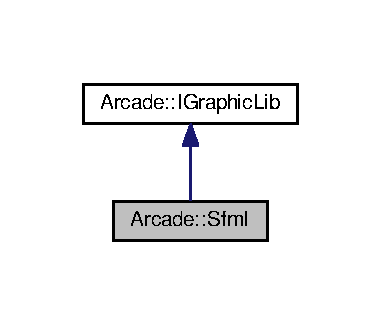
\includegraphics[width=183pt]{class_arcade_1_1_sfml__inherit__graph}
\end{center}
\end{figure}


Collaboration diagram for Arcade\+:\+:Sfml\+:
\nopagebreak
\begin{figure}[H]
\begin{center}
\leavevmode
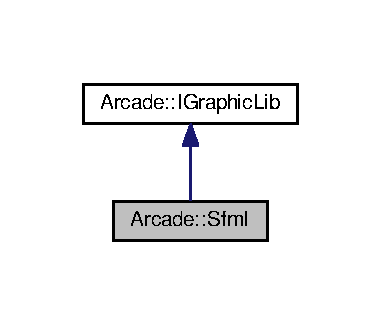
\includegraphics[width=183pt]{class_arcade_1_1_sfml__coll__graph}
\end{center}
\end{figure}
\subsection*{Public Member Functions}
\begin{DoxyCompactItemize}
\item 
std\+::string \hyperlink{class_arcade_1_1_sfml_a6c5776e27ea7466208ab4bd59395e344}{get\+Name} () const final
\begin{DoxyCompactList}\small\item\em Graphic library name\textquotesingle{}s getter. \end{DoxyCompactList}\item 
bool \hyperlink{class_arcade_1_1_sfml_a427b6fc608c3b52f167b1fe79f5a5009}{is\+Open} () const final
\begin{DoxyCompactList}\small\item\em Specifies whether the window is open or not. \end{DoxyCompactList}\item 
void \hyperlink{class_arcade_1_1_sfml_a3a2c22328c9ae1cfd7a5af03663e00d0}{close\+Renderer} () final
\begin{DoxyCompactList}\small\item\em Closes the rendering support. \end{DoxyCompactList}\item 
void \hyperlink{class_arcade_1_1_sfml_a9a868d1964ac2f24327329af971fdb57}{open\+Renderer} (std\+::string const \&title) final
\begin{DoxyCompactList}\small\item\em Opens the rendering support. \end{DoxyCompactList}\item 
\mbox{\Hypertarget{class_arcade_1_1_sfml_aebb824de8210e60ac67a63f6e4252f49}\label{class_arcade_1_1_sfml_aebb824de8210e60ac67a63f6e4252f49}} 
void \hyperlink{class_arcade_1_1_sfml_aebb824de8210e60ac67a63f6e4252f49}{clear\+Window} () final
\begin{DoxyCompactList}\small\item\em Clears the rendering support. \end{DoxyCompactList}\item 
\mbox{\Hypertarget{class_arcade_1_1_sfml_afbd4c271aa922955ad0131bf7d797acb}\label{class_arcade_1_1_sfml_afbd4c271aa922955ad0131bf7d797acb}} 
void \hyperlink{class_arcade_1_1_sfml_afbd4c271aa922955ad0131bf7d797acb}{refresh\+Window} () final
\begin{DoxyCompactList}\small\item\em Displays the buffered frame to the screen. \end{DoxyCompactList}\item 
\mbox{\Hypertarget{class_arcade_1_1_sfml_aab746ab375cb731196d8ceea9b0f627a}\label{class_arcade_1_1_sfml_aab746ab375cb731196d8ceea9b0f627a}} 
void \hyperlink{class_arcade_1_1_sfml_aab746ab375cb731196d8ceea9b0f627a}{draw\+Pixel\+Box} (\hyperlink{class_arcade_1_1_pixel_box}{Pixel\+Box} const \&) final
\begin{DoxyCompactList}\small\item\em Draws a \hyperlink{class_arcade_1_1_pixel_box}{Pixel\+Box}. \end{DoxyCompactList}\item 
\mbox{\Hypertarget{class_arcade_1_1_sfml_a9c627d2681c67a4118e6c0c167973ddc}\label{class_arcade_1_1_sfml_a9c627d2681c67a4118e6c0c167973ddc}} 
void \hyperlink{class_arcade_1_1_sfml_a9c627d2681c67a4118e6c0c167973ddc}{draw\+Text} (\hyperlink{class_arcade_1_1_text_box}{Text\+Box} const \&) final
\begin{DoxyCompactList}\small\item\em Draws a \hyperlink{class_arcade_1_1_text_box}{Text\+Box}. \end{DoxyCompactList}\item 
bool \hyperlink{class_arcade_1_1_sfml_a7b5fe6ccf84db8b3f2897805c965e607}{poll\+Events} () final
\begin{DoxyCompactList}\small\item\em Fetches the events from the user and saves it. \end{DoxyCompactList}\item 
\hyperlink{namespace_arcade_a9b501908b20bc993e4f8226db5323c41}{Keys} \hyperlink{class_arcade_1_1_sfml_aa31ab4c4729ee0e3ff030989bc38237b}{get\+Last\+Event} () final
\begin{DoxyCompactList}\small\item\em Getter of the oldest command in memory. \end{DoxyCompactList}\item 
void \hyperlink{class_arcade_1_1_sfml_a882877eba4037ffe3befd61a4b4f1d18}{clear\+Events} () final
\begin{DoxyCompactList}\small\item\em Clears the pending commands. \end{DoxyCompactList}\item 
\hyperlink{class_arcade_1_1_vect}{Vect}$<$ size\+\_\+t $>$ \hyperlink{class_arcade_1_1_sfml_aa2fe7257182649ba0273712d36296460}{get\+Screen\+Size} () const final
\begin{DoxyCompactList}\small\item\em Getter from the rendering support dimensions. \end{DoxyCompactList}\item 
size\+\_\+t \hyperlink{class_arcade_1_1_sfml_a90cb12cc852a0198074f55be843d6f99}{get\+MaxY} () const final
\begin{DoxyCompactList}\small\item\em Getter from the rendering support height. \end{DoxyCompactList}\item 
size\+\_\+t \hyperlink{class_arcade_1_1_sfml_a220fc84bb5728f79e36024fded0103ab}{get\+MaxX} () const final
\begin{DoxyCompactList}\small\item\em Getter from the rendering support width. \end{DoxyCompactList}\end{DoxyCompactItemize}


\subsection{Member Function Documentation}
\mbox{\Hypertarget{class_arcade_1_1_sfml_a882877eba4037ffe3befd61a4b4f1d18}\label{class_arcade_1_1_sfml_a882877eba4037ffe3befd61a4b4f1d18}} 
\index{Arcade\+::\+Sfml@{Arcade\+::\+Sfml}!clear\+Events@{clear\+Events}}
\index{clear\+Events@{clear\+Events}!Arcade\+::\+Sfml@{Arcade\+::\+Sfml}}
\subsubsection{\texorpdfstring{clear\+Events()}{clearEvents()}}
{\footnotesize\ttfamily void Arcade\+::\+Sfml\+::clear\+Events (\begin{DoxyParamCaption}{ }\end{DoxyParamCaption})\hspace{0.3cm}{\ttfamily [final]}, {\ttfamily [virtual]}}



Clears the pending commands. 

The function deletes all the commands currently stored. They wont be accessible anymore, even with the \hyperlink{class_arcade_1_1_sfml_aa31ab4c4729ee0e3ff030989bc38237b}{get\+Last\+Event()} method. 

Implements \hyperlink{class_arcade_1_1_i_graphic_lib_a78691f8f9433b2af945576231534c1e3}{Arcade\+::\+I\+Graphic\+Lib}.

\mbox{\Hypertarget{class_arcade_1_1_sfml_a3a2c22328c9ae1cfd7a5af03663e00d0}\label{class_arcade_1_1_sfml_a3a2c22328c9ae1cfd7a5af03663e00d0}} 
\index{Arcade\+::\+Sfml@{Arcade\+::\+Sfml}!close\+Renderer@{close\+Renderer}}
\index{close\+Renderer@{close\+Renderer}!Arcade\+::\+Sfml@{Arcade\+::\+Sfml}}
\subsubsection{\texorpdfstring{close\+Renderer()}{closeRenderer()}}
{\footnotesize\ttfamily void Arcade\+::\+Sfml\+::close\+Renderer (\begin{DoxyParamCaption}{ }\end{DoxyParamCaption})\hspace{0.3cm}{\ttfamily [final]}, {\ttfamily [virtual]}}



Closes the rendering support. 

Usually closes a window. Some graphic library uses other rendering support. 

Implements \hyperlink{class_arcade_1_1_i_graphic_lib_aa7c3c8b922fbc94f5e74ecfebad52742}{Arcade\+::\+I\+Graphic\+Lib}.

\mbox{\Hypertarget{class_arcade_1_1_sfml_aa31ab4c4729ee0e3ff030989bc38237b}\label{class_arcade_1_1_sfml_aa31ab4c4729ee0e3ff030989bc38237b}} 
\index{Arcade\+::\+Sfml@{Arcade\+::\+Sfml}!get\+Last\+Event@{get\+Last\+Event}}
\index{get\+Last\+Event@{get\+Last\+Event}!Arcade\+::\+Sfml@{Arcade\+::\+Sfml}}
\subsubsection{\texorpdfstring{get\+Last\+Event()}{getLastEvent()}}
{\footnotesize\ttfamily \hyperlink{namespace_arcade_a9b501908b20bc993e4f8226db5323c41}{Arcade\+::\+Keys} Arcade\+::\+Sfml\+::get\+Last\+Event (\begin{DoxyParamCaption}{ }\end{DoxyParamCaption})\hspace{0.3cm}{\ttfamily [final]}, {\ttfamily [virtual]}}



Getter of the oldest command in memory. 

\begin{DoxyReturn}{Returns}
the first event of the list.
\end{DoxyReturn}
The function deletes the command if it succeed to retrieves one, using front() and pop\+\_\+front() methods 

Implements \hyperlink{class_arcade_1_1_i_graphic_lib_a801ebd3cff2c861e4b2a1e664c123da7}{Arcade\+::\+I\+Graphic\+Lib}.

\mbox{\Hypertarget{class_arcade_1_1_sfml_a220fc84bb5728f79e36024fded0103ab}\label{class_arcade_1_1_sfml_a220fc84bb5728f79e36024fded0103ab}} 
\index{Arcade\+::\+Sfml@{Arcade\+::\+Sfml}!get\+MaxX@{get\+MaxX}}
\index{get\+MaxX@{get\+MaxX}!Arcade\+::\+Sfml@{Arcade\+::\+Sfml}}
\subsubsection{\texorpdfstring{get\+Max\+X()}{getMaxX()}}
{\footnotesize\ttfamily size\+\_\+t Arcade\+::\+Sfml\+::get\+MaxX (\begin{DoxyParamCaption}{ }\end{DoxyParamCaption}) const\hspace{0.3cm}{\ttfamily [final]}, {\ttfamily [virtual]}}



Getter from the rendering support width. 

\begin{DoxyReturn}{Returns}
the width of the rendering support 
\end{DoxyReturn}


Implements \hyperlink{class_arcade_1_1_i_graphic_lib_a41a3c00970ecd16e1893105de2091a55}{Arcade\+::\+I\+Graphic\+Lib}.

\mbox{\Hypertarget{class_arcade_1_1_sfml_a90cb12cc852a0198074f55be843d6f99}\label{class_arcade_1_1_sfml_a90cb12cc852a0198074f55be843d6f99}} 
\index{Arcade\+::\+Sfml@{Arcade\+::\+Sfml}!get\+MaxY@{get\+MaxY}}
\index{get\+MaxY@{get\+MaxY}!Arcade\+::\+Sfml@{Arcade\+::\+Sfml}}
\subsubsection{\texorpdfstring{get\+Max\+Y()}{getMaxY()}}
{\footnotesize\ttfamily size\+\_\+t Arcade\+::\+Sfml\+::get\+MaxY (\begin{DoxyParamCaption}{ }\end{DoxyParamCaption}) const\hspace{0.3cm}{\ttfamily [final]}, {\ttfamily [virtual]}}



Getter from the rendering support height. 

\begin{DoxyReturn}{Returns}
the height of the rendering support 
\end{DoxyReturn}


Implements \hyperlink{class_arcade_1_1_i_graphic_lib_ae8701e702b51189c84b1900dd624912e}{Arcade\+::\+I\+Graphic\+Lib}.

\mbox{\Hypertarget{class_arcade_1_1_sfml_a6c5776e27ea7466208ab4bd59395e344}\label{class_arcade_1_1_sfml_a6c5776e27ea7466208ab4bd59395e344}} 
\index{Arcade\+::\+Sfml@{Arcade\+::\+Sfml}!get\+Name@{get\+Name}}
\index{get\+Name@{get\+Name}!Arcade\+::\+Sfml@{Arcade\+::\+Sfml}}
\subsubsection{\texorpdfstring{get\+Name()}{getName()}}
{\footnotesize\ttfamily std\+::string Arcade\+::\+Sfml\+::get\+Name (\begin{DoxyParamCaption}{ }\end{DoxyParamCaption}) const\hspace{0.3cm}{\ttfamily [final]}, {\ttfamily [virtual]}}



Graphic library name\textquotesingle{}s getter. 

\begin{DoxyReturn}{Returns}
a string containing the name of the graphic library 
\end{DoxyReturn}


Implements \hyperlink{class_arcade_1_1_i_graphic_lib_aecc266c4ac10f07f4cdca023e74e843d}{Arcade\+::\+I\+Graphic\+Lib}.

\mbox{\Hypertarget{class_arcade_1_1_sfml_aa2fe7257182649ba0273712d36296460}\label{class_arcade_1_1_sfml_aa2fe7257182649ba0273712d36296460}} 
\index{Arcade\+::\+Sfml@{Arcade\+::\+Sfml}!get\+Screen\+Size@{get\+Screen\+Size}}
\index{get\+Screen\+Size@{get\+Screen\+Size}!Arcade\+::\+Sfml@{Arcade\+::\+Sfml}}
\subsubsection{\texorpdfstring{get\+Screen\+Size()}{getScreenSize()}}
{\footnotesize\ttfamily \hyperlink{class_arcade_1_1_vect}{Arcade\+::\+Vect}$<$ size\+\_\+t $>$ Arcade\+::\+Sfml\+::get\+Screen\+Size (\begin{DoxyParamCaption}{ }\end{DoxyParamCaption}) const\hspace{0.3cm}{\ttfamily [final]}, {\ttfamily [virtual]}}



Getter from the rendering support dimensions. 

\begin{DoxyReturn}{Returns}
a two dimensions vector containing the width and the height of the rendering support 
\end{DoxyReturn}


Implements \hyperlink{class_arcade_1_1_i_graphic_lib_a0ce5eb4661d55b6e729fc1c16566dd9f}{Arcade\+::\+I\+Graphic\+Lib}.

\mbox{\Hypertarget{class_arcade_1_1_sfml_a427b6fc608c3b52f167b1fe79f5a5009}\label{class_arcade_1_1_sfml_a427b6fc608c3b52f167b1fe79f5a5009}} 
\index{Arcade\+::\+Sfml@{Arcade\+::\+Sfml}!is\+Open@{is\+Open}}
\index{is\+Open@{is\+Open}!Arcade\+::\+Sfml@{Arcade\+::\+Sfml}}
\subsubsection{\texorpdfstring{is\+Open()}{isOpen()}}
{\footnotesize\ttfamily bool Arcade\+::\+Sfml\+::is\+Open (\begin{DoxyParamCaption}{ }\end{DoxyParamCaption}) const\hspace{0.3cm}{\ttfamily [final]}, {\ttfamily [virtual]}}



Specifies whether the window is open or not. 

\begin{DoxyReturn}{Returns}
true if open, otherwise returns false 
\end{DoxyReturn}


Implements \hyperlink{class_arcade_1_1_i_graphic_lib_adf9e107fbcfbd91e5a3daa9a2db76b4b}{Arcade\+::\+I\+Graphic\+Lib}.

\mbox{\Hypertarget{class_arcade_1_1_sfml_a9a868d1964ac2f24327329af971fdb57}\label{class_arcade_1_1_sfml_a9a868d1964ac2f24327329af971fdb57}} 
\index{Arcade\+::\+Sfml@{Arcade\+::\+Sfml}!open\+Renderer@{open\+Renderer}}
\index{open\+Renderer@{open\+Renderer}!Arcade\+::\+Sfml@{Arcade\+::\+Sfml}}
\subsubsection{\texorpdfstring{open\+Renderer()}{openRenderer()}}
{\footnotesize\ttfamily void Arcade\+::\+Sfml\+::open\+Renderer (\begin{DoxyParamCaption}\item[{std\+::string const \&}]{title }\end{DoxyParamCaption})\hspace{0.3cm}{\ttfamily [final]}, {\ttfamily [virtual]}}



Opens the rendering support. 


\begin{DoxyParams}{Parameters}
{\em title} & \+: Title of the rendering support if supported\\
\hline
\end{DoxyParams}
Usually opens a window. Some graphic library uses other rendering support. 

Implements \hyperlink{class_arcade_1_1_i_graphic_lib_a71f7f51bdd61b02377c4a9ec330eabb1}{Arcade\+::\+I\+Graphic\+Lib}.

\mbox{\Hypertarget{class_arcade_1_1_sfml_a7b5fe6ccf84db8b3f2897805c965e607}\label{class_arcade_1_1_sfml_a7b5fe6ccf84db8b3f2897805c965e607}} 
\index{Arcade\+::\+Sfml@{Arcade\+::\+Sfml}!poll\+Events@{poll\+Events}}
\index{poll\+Events@{poll\+Events}!Arcade\+::\+Sfml@{Arcade\+::\+Sfml}}
\subsubsection{\texorpdfstring{poll\+Events()}{pollEvents()}}
{\footnotesize\ttfamily bool Arcade\+::\+Sfml\+::poll\+Events (\begin{DoxyParamCaption}{ }\end{DoxyParamCaption})\hspace{0.3cm}{\ttfamily [final]}, {\ttfamily [virtual]}}



Fetches the events from the user and saves it. 

\begin{DoxyReturn}{Returns}
true if at least one command has been fetched, otherwise returns false
\end{DoxyReturn}
Fetched commands are usually stored inside a std\+::vector$<$\+Arcade\+::\+Keys$>$ or std\+::list$<$\+Arcade\+::\+Keys$>$ 

Implements \hyperlink{class_arcade_1_1_i_graphic_lib_a6be852f0395f08943f988c6823b80937}{Arcade\+::\+I\+Graphic\+Lib}.



The documentation for this class was generated from the following files\+:\begin{DoxyCompactItemize}
\item 
/home/rectoria/projects/epitech/\+C\+P\+P/cpp\+\_\+arcade/lib/\+S\+F\+M\+L/Sfml.\+hpp\item 
/home/rectoria/projects/epitech/\+C\+P\+P/cpp\+\_\+arcade/lib/\+S\+F\+M\+L/Sfml.\+cpp\end{DoxyCompactItemize}

\hypertarget{class_arcade_1_1_text_box}{}\section{Arcade\+:\+:Text\+Box Class Reference}
\label{class_arcade_1_1_text_box}\index{Arcade\+::\+Text\+Box@{Arcade\+::\+Text\+Box}}


\hyperlink{class_arcade_1_1_text_box}{Text\+Box} class.  




{\ttfamily \#include $<$Text\+Box.\+hpp$>$}

\subsection*{Public Member Functions}
\begin{DoxyCompactItemize}
\item 
\hyperlink{class_arcade_1_1_text_box_ad906f51406be8703146d7fe4eac0a7df}{Text\+Box} (std\+::string const \&text, \hyperlink{class_arcade_1_1_vect}{Vect}$<$ size\+\_\+t $>$ pos, size\+\_\+t font\+Size=30, \hyperlink{class_arcade_1_1_color}{Color} color=\hyperlink{class_arcade_1_1_color}{Color}(255, 255, 255, 255), \hyperlink{class_arcade_1_1_color}{Color} background\+Color=\hyperlink{class_arcade_1_1_color}{Color}(0, 0, 0, 255))
\begin{DoxyCompactList}\small\item\em \hyperlink{class_arcade_1_1_text_box}{Text\+Box} class\textquotesingle{}s constructor. \end{DoxyCompactList}\item 
\mbox{\Hypertarget{class_arcade_1_1_text_box_a8c3f24e683f3ed4a0b26dfb058077fca}\label{class_arcade_1_1_text_box_a8c3f24e683f3ed4a0b26dfb058077fca}} 
\hyperlink{class_arcade_1_1_text_box_a8c3f24e683f3ed4a0b26dfb058077fca}{$\sim$\+Text\+Box} ()=default
\begin{DoxyCompactList}\small\item\em \hyperlink{class_arcade_1_1_pixel_box}{Pixel\+Box} class\textquotesingle{}s destructor. \end{DoxyCompactList}\item 
const std\+::string \& \hyperlink{class_arcade_1_1_text_box_a08d2b7ad04db74670557a2136db06add}{get\+Value} () const
\begin{DoxyCompactList}\small\item\em \hyperlink{class_arcade_1_1_text_box}{Text\+Box} text\textquotesingle{}s value\textquotesingle{}s getter. \end{DoxyCompactList}\item 
void \hyperlink{class_arcade_1_1_text_box_a195c78d58c25c9f8a810a0ae7450220f}{set\+Value} (std\+::string const \&text)
\begin{DoxyCompactList}\small\item\em Sets the text\+Box text\textquotesingle{}s value. \end{DoxyCompactList}\item 
\hyperlink{class_arcade_1_1_vect}{Vect}$<$ size\+\_\+t $>$ \hyperlink{class_arcade_1_1_text_box_aaaf37e50180337a66b0895bffce126b7}{get\+Pos} () const
\begin{DoxyCompactList}\small\item\em \hyperlink{class_arcade_1_1_text_box}{Text\+Box} positions\textquotesingle{}s getter. \end{DoxyCompactList}\item 
void \hyperlink{class_arcade_1_1_text_box_aec7043b5dc883feed62a8e8eb9dea78d}{set\+Pos} (\hyperlink{class_arcade_1_1_vect}{Vect}$<$ size\+\_\+t $>$ pos)
\begin{DoxyCompactList}\small\item\em \hyperlink{class_arcade_1_1_text_box}{Text\+Box} positions\textquotesingle{}s setter. \end{DoxyCompactList}\item 
\mbox{\Hypertarget{class_arcade_1_1_text_box_a0aba97e86b30ab14a0ba65a0ffc80b42}\label{class_arcade_1_1_text_box_a0aba97e86b30ab14a0ba65a0ffc80b42}} 
size\+\_\+t \hyperlink{class_arcade_1_1_text_box_a0aba97e86b30ab14a0ba65a0ffc80b42}{getX} () const
\begin{DoxyCompactList}\small\item\em \hyperlink{class_arcade_1_1_text_box}{Text\+Box} X offset\textquotesingle{}s getter. \end{DoxyCompactList}\item 
\mbox{\Hypertarget{class_arcade_1_1_text_box_a39794a2a5799911e0f7ebb53082e05bc}\label{class_arcade_1_1_text_box_a39794a2a5799911e0f7ebb53082e05bc}} 
size\+\_\+t \hyperlink{class_arcade_1_1_text_box_a39794a2a5799911e0f7ebb53082e05bc}{getY} () const
\begin{DoxyCompactList}\small\item\em \hyperlink{class_arcade_1_1_text_box}{Text\+Box} Y offset\textquotesingle{}s getter. \end{DoxyCompactList}\item 
\mbox{\Hypertarget{class_arcade_1_1_text_box_aee7fe4770c6ccb3776f8bc4cb56b6208}\label{class_arcade_1_1_text_box_aee7fe4770c6ccb3776f8bc4cb56b6208}} 
void \hyperlink{class_arcade_1_1_text_box_aee7fe4770c6ccb3776f8bc4cb56b6208}{setX} (size\+\_\+t x)
\begin{DoxyCompactList}\small\item\em \hyperlink{class_arcade_1_1_text_box}{Text\+Box} X offset\textquotesingle{}s setter. \end{DoxyCompactList}\item 
\mbox{\Hypertarget{class_arcade_1_1_text_box_a0e0f2432518b99b4aea3503f99833abc}\label{class_arcade_1_1_text_box_a0e0f2432518b99b4aea3503f99833abc}} 
void \hyperlink{class_arcade_1_1_text_box_a0e0f2432518b99b4aea3503f99833abc}{setY} (size\+\_\+t y)
\begin{DoxyCompactList}\small\item\em \hyperlink{class_arcade_1_1_text_box}{Text\+Box} Y offset\textquotesingle{}s setter. \end{DoxyCompactList}\item 
size\+\_\+t \hyperlink{class_arcade_1_1_text_box_a8b8735d3c752067da9fc88f1e5fe1164}{get\+Font\+Size} () const
\begin{DoxyCompactList}\small\item\em \hyperlink{class_arcade_1_1_text_box}{Text\+Box}\textquotesingle{}s font size\textquotesingle{}s getter. \end{DoxyCompactList}\item 
void \hyperlink{class_arcade_1_1_text_box_ad65297c8da7cf939ee635191269f4440}{set\+Font\+Size} (size\+\_\+t size)
\begin{DoxyCompactList}\small\item\em \hyperlink{class_arcade_1_1_text_box}{Text\+Box}\textquotesingle{}s font size\textquotesingle{}s setter. \end{DoxyCompactList}\item 
\hyperlink{class_arcade_1_1_color}{Color} \hyperlink{class_arcade_1_1_text_box_a5fb50d6e6e1b2145a39b962ebd1016c7}{get\+Color} () const
\begin{DoxyCompactList}\small\item\em \hyperlink{class_arcade_1_1_text_box}{Text\+Box}\textquotesingle{}s text color\textquotesingle{}s getter. \end{DoxyCompactList}\item 
void \hyperlink{class_arcade_1_1_text_box_acd8eccc744d276c3be9a16facf7449b7}{set\+Color} (\hyperlink{class_arcade_1_1_color}{Color} color)
\begin{DoxyCompactList}\small\item\em \hyperlink{class_arcade_1_1_text_box}{Text\+Box}\textquotesingle{}s text color\textquotesingle{}s setter. \end{DoxyCompactList}\item 
\hyperlink{class_arcade_1_1_color}{Color} \hyperlink{class_arcade_1_1_text_box_ab7f4529da65dcab7508563e32c55ddbe}{get\+Background\+Color} () const
\begin{DoxyCompactList}\small\item\em \hyperlink{class_arcade_1_1_text_box}{Text\+Box}\textquotesingle{}s text background color\textquotesingle{}s getter. \end{DoxyCompactList}\item 
void \hyperlink{class_arcade_1_1_text_box_a01f432d437ec9500bb8fc6383765f90b}{set\+Background\+Color} (\hyperlink{class_arcade_1_1_color}{Color} color)
\begin{DoxyCompactList}\small\item\em \hyperlink{class_arcade_1_1_text_box}{Text\+Box}\textquotesingle{}s text background color\textquotesingle{}s setter. \end{DoxyCompactList}\end{DoxyCompactItemize}


\subsection{Detailed Description}
\hyperlink{class_arcade_1_1_text_box}{Text\+Box} class. 

Class used to represent a rectangle of text 

\subsection{Constructor \& Destructor Documentation}
\mbox{\Hypertarget{class_arcade_1_1_text_box_ad906f51406be8703146d7fe4eac0a7df}\label{class_arcade_1_1_text_box_ad906f51406be8703146d7fe4eac0a7df}} 
\index{Arcade\+::\+Text\+Box@{Arcade\+::\+Text\+Box}!Text\+Box@{Text\+Box}}
\index{Text\+Box@{Text\+Box}!Arcade\+::\+Text\+Box@{Arcade\+::\+Text\+Box}}
\subsubsection{\texorpdfstring{Text\+Box()}{TextBox()}}
{\footnotesize\ttfamily Arcade\+::\+Text\+Box\+::\+Text\+Box (\begin{DoxyParamCaption}\item[{std\+::string const \&}]{text,  }\item[{\hyperlink{class_arcade_1_1_vect}{Arcade\+::\+Vect}$<$ size\+\_\+t $>$}]{pos,  }\item[{size\+\_\+t}]{font\+Size = {\ttfamily 30},  }\item[{\hyperlink{class_arcade_1_1_color}{Arcade\+::\+Color}}]{color = {\ttfamily \hyperlink{class_arcade_1_1_color}{Color}(255,~255,~255,~255)},  }\item[{\hyperlink{class_arcade_1_1_color}{Arcade\+::\+Color}}]{background\+Color = {\ttfamily \hyperlink{class_arcade_1_1_color}{Color}(0,~0,~0,~255)} }\end{DoxyParamCaption})}



\hyperlink{class_arcade_1_1_text_box}{Text\+Box} class\textquotesingle{}s constructor. 


\begin{DoxyParams}{Parameters}
{\em text} & \+: characters to be apply on the text\+Box \\
\hline
{\em pos} & \+: \hyperlink{class_arcade_1_1_vect}{Vect$<$size\+\_\+t$>$} containing both x and y offsets. Used to place the text\+Box on the rendering support \\
\hline
{\em font\+Size} & \+: size of the text \\
\hline
{\em color} & \+: color of the text \\
\hline
{\em background\+Color} & \+: background color of the text\\
\hline
\end{DoxyParams}
Creates a new text\+Box class instance. The first text argument defines the value of the text within the text\+Box. The \hyperlink{class_arcade_1_1_vect}{Vect$<$size\+\_\+t$>$} pos argument defines the coordinates of the text\+Box\textquotesingle{}s position on the rendering support. It will be the offset applied when rendering it. The third font\+Size argument defines the size in which the text should be printed. The color\textquotesingle{}s argument defines in which color the characters will be printed. The background\+Color\textquotesingle{}s argument defines the background color of the characters. 

\subsection{Member Function Documentation}
\mbox{\Hypertarget{class_arcade_1_1_text_box_ab7f4529da65dcab7508563e32c55ddbe}\label{class_arcade_1_1_text_box_ab7f4529da65dcab7508563e32c55ddbe}} 
\index{Arcade\+::\+Text\+Box@{Arcade\+::\+Text\+Box}!get\+Background\+Color@{get\+Background\+Color}}
\index{get\+Background\+Color@{get\+Background\+Color}!Arcade\+::\+Text\+Box@{Arcade\+::\+Text\+Box}}
\subsubsection{\texorpdfstring{get\+Background\+Color()}{getBackgroundColor()}}
{\footnotesize\ttfamily \hyperlink{class_arcade_1_1_color}{Arcade\+::\+Color} Arcade\+::\+Text\+Box\+::get\+Background\+Color (\begin{DoxyParamCaption}{ }\end{DoxyParamCaption}) const}



\hyperlink{class_arcade_1_1_text_box}{Text\+Box}\textquotesingle{}s text background color\textquotesingle{}s getter. 

\begin{DoxyReturn}{Returns}
the text\+Box\textquotesingle{}s text\textquotesingle{}s background color 
\end{DoxyReturn}
\mbox{\Hypertarget{class_arcade_1_1_text_box_a5fb50d6e6e1b2145a39b962ebd1016c7}\label{class_arcade_1_1_text_box_a5fb50d6e6e1b2145a39b962ebd1016c7}} 
\index{Arcade\+::\+Text\+Box@{Arcade\+::\+Text\+Box}!get\+Color@{get\+Color}}
\index{get\+Color@{get\+Color}!Arcade\+::\+Text\+Box@{Arcade\+::\+Text\+Box}}
\subsubsection{\texorpdfstring{get\+Color()}{getColor()}}
{\footnotesize\ttfamily \hyperlink{class_arcade_1_1_color}{Arcade\+::\+Color} Arcade\+::\+Text\+Box\+::get\+Color (\begin{DoxyParamCaption}{ }\end{DoxyParamCaption}) const}



\hyperlink{class_arcade_1_1_text_box}{Text\+Box}\textquotesingle{}s text color\textquotesingle{}s getter. 

\begin{DoxyReturn}{Returns}
the text\+Box\textquotesingle{}s text\textquotesingle{}s color 
\end{DoxyReturn}
\mbox{\Hypertarget{class_arcade_1_1_text_box_a8b8735d3c752067da9fc88f1e5fe1164}\label{class_arcade_1_1_text_box_a8b8735d3c752067da9fc88f1e5fe1164}} 
\index{Arcade\+::\+Text\+Box@{Arcade\+::\+Text\+Box}!get\+Font\+Size@{get\+Font\+Size}}
\index{get\+Font\+Size@{get\+Font\+Size}!Arcade\+::\+Text\+Box@{Arcade\+::\+Text\+Box}}
\subsubsection{\texorpdfstring{get\+Font\+Size()}{getFontSize()}}
{\footnotesize\ttfamily size\+\_\+t Arcade\+::\+Text\+Box\+::get\+Font\+Size (\begin{DoxyParamCaption}{ }\end{DoxyParamCaption}) const}



\hyperlink{class_arcade_1_1_text_box}{Text\+Box}\textquotesingle{}s font size\textquotesingle{}s getter. 

\begin{DoxyReturn}{Returns}
the font size 
\end{DoxyReturn}
\mbox{\Hypertarget{class_arcade_1_1_text_box_aaaf37e50180337a66b0895bffce126b7}\label{class_arcade_1_1_text_box_aaaf37e50180337a66b0895bffce126b7}} 
\index{Arcade\+::\+Text\+Box@{Arcade\+::\+Text\+Box}!get\+Pos@{get\+Pos}}
\index{get\+Pos@{get\+Pos}!Arcade\+::\+Text\+Box@{Arcade\+::\+Text\+Box}}
\subsubsection{\texorpdfstring{get\+Pos()}{getPos()}}
{\footnotesize\ttfamily \hyperlink{class_arcade_1_1_vect}{Arcade\+::\+Vect}$<$ size\+\_\+t $>$ Arcade\+::\+Text\+Box\+::get\+Pos (\begin{DoxyParamCaption}{ }\end{DoxyParamCaption}) const}



\hyperlink{class_arcade_1_1_text_box}{Text\+Box} positions\textquotesingle{}s getter. 

\begin{DoxyReturn}{Returns}
a \hyperlink{class_arcade_1_1_vect}{Vect$<$size\+\_\+t$>$} containing the offsetX (x) and the offsetY (y) of the text\+Box. 
\end{DoxyReturn}
\mbox{\Hypertarget{class_arcade_1_1_text_box_a08d2b7ad04db74670557a2136db06add}\label{class_arcade_1_1_text_box_a08d2b7ad04db74670557a2136db06add}} 
\index{Arcade\+::\+Text\+Box@{Arcade\+::\+Text\+Box}!get\+Value@{get\+Value}}
\index{get\+Value@{get\+Value}!Arcade\+::\+Text\+Box@{Arcade\+::\+Text\+Box}}
\subsubsection{\texorpdfstring{get\+Value()}{getValue()}}
{\footnotesize\ttfamily const std\+::string \& Arcade\+::\+Text\+Box\+::get\+Value (\begin{DoxyParamCaption}{ }\end{DoxyParamCaption}) const}



\hyperlink{class_arcade_1_1_text_box}{Text\+Box} text\textquotesingle{}s value\textquotesingle{}s getter. 

\begin{DoxyReturn}{Returns}
the value of the text within text\+Box 
\end{DoxyReturn}
\mbox{\Hypertarget{class_arcade_1_1_text_box_a01f432d437ec9500bb8fc6383765f90b}\label{class_arcade_1_1_text_box_a01f432d437ec9500bb8fc6383765f90b}} 
\index{Arcade\+::\+Text\+Box@{Arcade\+::\+Text\+Box}!set\+Background\+Color@{set\+Background\+Color}}
\index{set\+Background\+Color@{set\+Background\+Color}!Arcade\+::\+Text\+Box@{Arcade\+::\+Text\+Box}}
\subsubsection{\texorpdfstring{set\+Background\+Color()}{setBackgroundColor()}}
{\footnotesize\ttfamily void Arcade\+::\+Text\+Box\+::set\+Background\+Color (\begin{DoxyParamCaption}\item[{\hyperlink{class_arcade_1_1_color}{Arcade\+::\+Color}}]{color }\end{DoxyParamCaption})}



\hyperlink{class_arcade_1_1_text_box}{Text\+Box}\textquotesingle{}s text background color\textquotesingle{}s setter. 


\begin{DoxyParams}{Parameters}
{\em color} & \+: new background color to apply to text \\
\hline
\end{DoxyParams}
\mbox{\Hypertarget{class_arcade_1_1_text_box_acd8eccc744d276c3be9a16facf7449b7}\label{class_arcade_1_1_text_box_acd8eccc744d276c3be9a16facf7449b7}} 
\index{Arcade\+::\+Text\+Box@{Arcade\+::\+Text\+Box}!set\+Color@{set\+Color}}
\index{set\+Color@{set\+Color}!Arcade\+::\+Text\+Box@{Arcade\+::\+Text\+Box}}
\subsubsection{\texorpdfstring{set\+Color()}{setColor()}}
{\footnotesize\ttfamily void Arcade\+::\+Text\+Box\+::set\+Color (\begin{DoxyParamCaption}\item[{\hyperlink{class_arcade_1_1_color}{Arcade\+::\+Color}}]{color }\end{DoxyParamCaption})}



\hyperlink{class_arcade_1_1_text_box}{Text\+Box}\textquotesingle{}s text color\textquotesingle{}s setter. 


\begin{DoxyParams}{Parameters}
{\em color} & \+: new color to apply to text \\
\hline
\end{DoxyParams}
\mbox{\Hypertarget{class_arcade_1_1_text_box_ad65297c8da7cf939ee635191269f4440}\label{class_arcade_1_1_text_box_ad65297c8da7cf939ee635191269f4440}} 
\index{Arcade\+::\+Text\+Box@{Arcade\+::\+Text\+Box}!set\+Font\+Size@{set\+Font\+Size}}
\index{set\+Font\+Size@{set\+Font\+Size}!Arcade\+::\+Text\+Box@{Arcade\+::\+Text\+Box}}
\subsubsection{\texorpdfstring{set\+Font\+Size()}{setFontSize()}}
{\footnotesize\ttfamily void Arcade\+::\+Text\+Box\+::set\+Font\+Size (\begin{DoxyParamCaption}\item[{size\+\_\+t}]{size }\end{DoxyParamCaption})}



\hyperlink{class_arcade_1_1_text_box}{Text\+Box}\textquotesingle{}s font size\textquotesingle{}s setter. 


\begin{DoxyParams}{Parameters}
{\em size} & \+: new font size to be assigned \\
\hline
\end{DoxyParams}
\mbox{\Hypertarget{class_arcade_1_1_text_box_aec7043b5dc883feed62a8e8eb9dea78d}\label{class_arcade_1_1_text_box_aec7043b5dc883feed62a8e8eb9dea78d}} 
\index{Arcade\+::\+Text\+Box@{Arcade\+::\+Text\+Box}!set\+Pos@{set\+Pos}}
\index{set\+Pos@{set\+Pos}!Arcade\+::\+Text\+Box@{Arcade\+::\+Text\+Box}}
\subsubsection{\texorpdfstring{set\+Pos()}{setPos()}}
{\footnotesize\ttfamily void Arcade\+::\+Text\+Box\+::set\+Pos (\begin{DoxyParamCaption}\item[{\hyperlink{class_arcade_1_1_vect}{Arcade\+::\+Vect}$<$ size\+\_\+t $>$}]{pos }\end{DoxyParamCaption})}



\hyperlink{class_arcade_1_1_text_box}{Text\+Box} positions\textquotesingle{}s setter. 


\begin{DoxyParams}{Parameters}
{\em pos} & \+: new positions of the text\+Box\\
\hline
\end{DoxyParams}
Takes both new positions as parameter, within a \hyperlink{class_arcade_1_1_vect}{Vect$<$size\+\_\+t$>$} \mbox{\Hypertarget{class_arcade_1_1_text_box_a195c78d58c25c9f8a810a0ae7450220f}\label{class_arcade_1_1_text_box_a195c78d58c25c9f8a810a0ae7450220f}} 
\index{Arcade\+::\+Text\+Box@{Arcade\+::\+Text\+Box}!set\+Value@{set\+Value}}
\index{set\+Value@{set\+Value}!Arcade\+::\+Text\+Box@{Arcade\+::\+Text\+Box}}
\subsubsection{\texorpdfstring{set\+Value()}{setValue()}}
{\footnotesize\ttfamily void Arcade\+::\+Text\+Box\+::set\+Value (\begin{DoxyParamCaption}\item[{std\+::string const \&}]{text }\end{DoxyParamCaption})}



Sets the text\+Box text\textquotesingle{}s value. 


\begin{DoxyParams}{Parameters}
{\em text} & \+: new value to assign \\
\hline
\end{DoxyParams}


The documentation for this class was generated from the following files\+:\begin{DoxyCompactItemize}
\item 
/home/rectoria/projects/epitech/\+C\+P\+P/cpp\+\_\+arcade/include/\hyperlink{_text_box_8hpp}{Text\+Box.\+hpp}\item 
/home/rectoria/projects/epitech/\+C\+P\+P/cpp\+\_\+arcade/include/Text\+Box.\+cpp\end{DoxyCompactItemize}

\hypertarget{class_arcade_1_1_vect}{}\section{Arcade\+:\+:Vect$<$ T $>$ Class Template Reference}
\label{class_arcade_1_1_vect}\index{Arcade\+::\+Vect$<$ T $>$@{Arcade\+::\+Vect$<$ T $>$}}


\hyperlink{class_arcade_1_1_vect}{Vect} class template.  




{\ttfamily \#include $<$Vect.\+hpp$>$}

\subsection*{Public Member Functions}
\begin{DoxyCompactItemize}
\item 
\hyperlink{class_arcade_1_1_vect_a9563cff4e95df68c9c39af00ba537d45}{Vect} (T x=0, T y=0)
\begin{DoxyCompactList}\small\item\em \hyperlink{class_arcade_1_1_vect}{Vect} class template\textquotesingle{}s constructor. \end{DoxyCompactList}\item 
void \hyperlink{class_arcade_1_1_vect_a08e707c4b986c33db4f1b1b749952bf3}{set\+XY} (T x=0, T y=0)
\begin{DoxyCompactList}\small\item\em \hyperlink{class_arcade_1_1_vect}{Vect} class template\textquotesingle{}s coordinates\textquotesingle{}s setter. \end{DoxyCompactList}\item 
void \hyperlink{class_arcade_1_1_vect_aa8eb2bf7c76a34771ebe1ee14b61028c}{setX} (T x=0)
\begin{DoxyCompactList}\small\item\em \hyperlink{class_arcade_1_1_vect}{Vect} class template\textquotesingle{}s X coordinate\textquotesingle{}s setter. \end{DoxyCompactList}\item 
void \hyperlink{class_arcade_1_1_vect_a4b4d15fd902f40d1e874471fb596612c}{setY} (T y=0)
\begin{DoxyCompactList}\small\item\em \hyperlink{class_arcade_1_1_vect}{Vect} class template\textquotesingle{}s Y coordinate\textquotesingle{}s setter. \end{DoxyCompactList}\item 
T \hyperlink{class_arcade_1_1_vect_a07237933a773c4f626a89415846886f1}{getX} () const
\begin{DoxyCompactList}\small\item\em \hyperlink{class_arcade_1_1_vect}{Vect} class template\textquotesingle{}s X coordinate\textquotesingle{}s getter. \end{DoxyCompactList}\item 
T \hyperlink{class_arcade_1_1_vect_a7d8b8821d45ff6faa5164f8cbccb0875}{getY} () const
\begin{DoxyCompactList}\small\item\em \hyperlink{class_arcade_1_1_vect}{Vect} class template\textquotesingle{}s Y coordinate\textquotesingle{}s getter. \end{DoxyCompactList}\item 
bool \hyperlink{class_arcade_1_1_vect_a553d8d71f49bd9623a1bfa6c01c28174}{operator==} (const \hyperlink{class_arcade_1_1_vect}{Vect}$<$ T $>$ \&other) const
\begin{DoxyCompactList}\small\item\em Overloading the comparison operator. \end{DoxyCompactList}\item 
\hyperlink{class_arcade_1_1_vect}{Vect}$<$ T $>$ \hyperlink{class_arcade_1_1_vect_a63deac98e5926a6a11901d4accb2c838}{operator+} (const \hyperlink{class_arcade_1_1_vect}{Vect}$<$ T $>$ \&other) const
\item 
\hyperlink{class_arcade_1_1_vect}{Vect}$<$ T $>$ \hyperlink{class_arcade_1_1_vect_a8dcc249d6a66e36cc75df3c809f2fd4f}{operator-\/} (const \hyperlink{class_arcade_1_1_vect}{Vect}$<$ T $>$ \&other) const
\item 
\hyperlink{class_arcade_1_1_vect}{Vect}$<$ T $>$ \hyperlink{class_arcade_1_1_vect_a81ec17a7c29e37edb411397070b71db2}{operator$\ast$} (const \hyperlink{class_arcade_1_1_vect}{Vect}$<$ T $>$ \&other) const
\item 
\hyperlink{class_arcade_1_1_vect}{Vect}$<$ T $>$ \hyperlink{class_arcade_1_1_vect_ae34d76a3387c62538f9c20c8acb42fa6}{operator/} (const \hyperlink{class_arcade_1_1_vect}{Vect}$<$ T $>$ \&other) const
\item 
\hyperlink{class_arcade_1_1_vect}{Vect}$<$ T $>$ \& \hyperlink{class_arcade_1_1_vect_a6ac5816789a378675e9d568327649e21}{operator+=} (const \hyperlink{class_arcade_1_1_vect}{Vect}$<$ T $>$ \&other)
\item 
\hyperlink{class_arcade_1_1_vect}{Vect}$<$ T $>$ \& \hyperlink{class_arcade_1_1_vect_a5e0919a6e98f86643268fd2270436d60}{operator-\/=} (const \hyperlink{class_arcade_1_1_vect}{Vect}$<$ T $>$ \&other)
\item 
\hyperlink{class_arcade_1_1_vect}{Vect}$<$ T $>$ \& \hyperlink{class_arcade_1_1_vect_a555efa11a995294522ab2f84455c2fea}{operator$\ast$=} (const \hyperlink{class_arcade_1_1_vect}{Vect}$<$ T $>$ \&other)
\item 
\hyperlink{class_arcade_1_1_vect}{Vect}$<$ T $>$ \& \hyperlink{class_arcade_1_1_vect_ae3114c792862c161769fbe2d1ce25df8}{operator/=} (const \hyperlink{class_arcade_1_1_vect}{Vect}$<$ T $>$ \&other)
\item 
\hyperlink{class_arcade_1_1_vect}{Vect}$<$ T $>$ \hyperlink{class_arcade_1_1_vect_ac03e7d5e4be634948b7a18541d8131ab}{operator+} (const T \&other) const
\item 
\hyperlink{class_arcade_1_1_vect}{Vect}$<$ T $>$ \hyperlink{class_arcade_1_1_vect_ae519ffdc7a4e3c79f7172df51bdf32c1}{operator-\/} (const T \&other) const
\item 
\hyperlink{class_arcade_1_1_vect}{Vect}$<$ T $>$ \hyperlink{class_arcade_1_1_vect_a88a56be9ee5a46ff58f08714315840ac}{operator$\ast$} (const T \&other) const
\item 
\hyperlink{class_arcade_1_1_vect}{Vect}$<$ T $>$ \hyperlink{class_arcade_1_1_vect_ad7cab0bc6711c2b9ec6aa5d11614f01e}{operator/} (const T \&other) const
\item 
\hyperlink{class_arcade_1_1_vect}{Vect}$<$ T $>$ \& \hyperlink{class_arcade_1_1_vect_a4da391cc6d6aaadc70819d7b50af6291}{operator+=} (const T \&other)
\item 
\hyperlink{class_arcade_1_1_vect}{Vect}$<$ T $>$ \& \hyperlink{class_arcade_1_1_vect_a0c2f3a86672b88f6baec98b5f2e9ad49}{operator-\/=} (const T \&other)
\item 
\hyperlink{class_arcade_1_1_vect}{Vect}$<$ T $>$ \& \hyperlink{class_arcade_1_1_vect_a64363c0a5ff75713a11174f48de1a8ea}{operator$\ast$=} (const T \&other)
\item 
\hyperlink{class_arcade_1_1_vect}{Vect}$<$ T $>$ \& \hyperlink{class_arcade_1_1_vect_a6777436fa526fb4397c169dd1a7fe6e5}{operator/=} (const T \&other)
\end{DoxyCompactItemize}


\subsection{Detailed Description}
\subsubsection*{template$<$typename T$>$\newline
class Arcade\+::\+Vect$<$ T $>$}

\hyperlink{class_arcade_1_1_vect}{Vect} class template. 

Mainly used to store and manage 2 coordinates 

\subsection{Constructor \& Destructor Documentation}
\mbox{\Hypertarget{class_arcade_1_1_vect_a9563cff4e95df68c9c39af00ba537d45}\label{class_arcade_1_1_vect_a9563cff4e95df68c9c39af00ba537d45}} 
\index{Arcade\+::\+Vect@{Arcade\+::\+Vect}!Vect@{Vect}}
\index{Vect@{Vect}!Arcade\+::\+Vect@{Arcade\+::\+Vect}}
\subsubsection{\texorpdfstring{Vect()}{Vect()}}
{\footnotesize\ttfamily template$<$typename T$>$ \\
\hyperlink{class_arcade_1_1_vect}{Arcade\+::\+Vect}$<$ T $>$\+::\hyperlink{class_arcade_1_1_vect}{Vect} (\begin{DoxyParamCaption}\item[{T}]{x = {\ttfamily 0},  }\item[{T}]{y = {\ttfamily 0} }\end{DoxyParamCaption})\hspace{0.3cm}{\ttfamily [inline]}, {\ttfamily [explicit]}}



\hyperlink{class_arcade_1_1_vect}{Vect} class template\textquotesingle{}s constructor. 


\begin{DoxyParams}{Parameters}
{\em x} & \+: coordinate X \\
\hline
{\em y} & \+: coordinate Y \\
\hline
\end{DoxyParams}


\subsection{Member Function Documentation}
\mbox{\Hypertarget{class_arcade_1_1_vect_a07237933a773c4f626a89415846886f1}\label{class_arcade_1_1_vect_a07237933a773c4f626a89415846886f1}} 
\index{Arcade\+::\+Vect@{Arcade\+::\+Vect}!getX@{getX}}
\index{getX@{getX}!Arcade\+::\+Vect@{Arcade\+::\+Vect}}
\subsubsection{\texorpdfstring{get\+X()}{getX()}}
{\footnotesize\ttfamily template$<$typename T$>$ \\
T \hyperlink{class_arcade_1_1_vect}{Arcade\+::\+Vect}$<$ T $>$\+::getX (\begin{DoxyParamCaption}{ }\end{DoxyParamCaption}) const\hspace{0.3cm}{\ttfamily [inline]}}



\hyperlink{class_arcade_1_1_vect}{Vect} class template\textquotesingle{}s X coordinate\textquotesingle{}s getter. 

\begin{DoxyReturn}{Returns}
the value of the X coordinate 
\end{DoxyReturn}
\mbox{\Hypertarget{class_arcade_1_1_vect_a7d8b8821d45ff6faa5164f8cbccb0875}\label{class_arcade_1_1_vect_a7d8b8821d45ff6faa5164f8cbccb0875}} 
\index{Arcade\+::\+Vect@{Arcade\+::\+Vect}!getY@{getY}}
\index{getY@{getY}!Arcade\+::\+Vect@{Arcade\+::\+Vect}}
\subsubsection{\texorpdfstring{get\+Y()}{getY()}}
{\footnotesize\ttfamily template$<$typename T$>$ \\
T \hyperlink{class_arcade_1_1_vect}{Arcade\+::\+Vect}$<$ T $>$\+::getY (\begin{DoxyParamCaption}{ }\end{DoxyParamCaption}) const\hspace{0.3cm}{\ttfamily [inline]}}



\hyperlink{class_arcade_1_1_vect}{Vect} class template\textquotesingle{}s Y coordinate\textquotesingle{}s getter. 

\begin{DoxyReturn}{Returns}
the value of the Y coordinate 
\end{DoxyReturn}
\mbox{\Hypertarget{class_arcade_1_1_vect_a81ec17a7c29e37edb411397070b71db2}\label{class_arcade_1_1_vect_a81ec17a7c29e37edb411397070b71db2}} 
\index{Arcade\+::\+Vect@{Arcade\+::\+Vect}!operator$\ast$@{operator$\ast$}}
\index{operator$\ast$@{operator$\ast$}!Arcade\+::\+Vect@{Arcade\+::\+Vect}}
\subsubsection{\texorpdfstring{operator$\ast$()}{operator*()}\hspace{0.1cm}{\footnotesize\ttfamily [1/2]}}
{\footnotesize\ttfamily template$<$typename T$>$ \\
\hyperlink{class_arcade_1_1_vect}{Vect}$<$T$>$ \hyperlink{class_arcade_1_1_vect}{Arcade\+::\+Vect}$<$ T $>$\+::operator$\ast$ (\begin{DoxyParamCaption}\item[{const \hyperlink{class_arcade_1_1_vect}{Vect}$<$ T $>$ \&}]{other }\end{DoxyParamCaption}) const\hspace{0.3cm}{\ttfamily [inline]}}

Overloading the multiplication operator 
\begin{DoxyParams}{Parameters}
{\em other} & \+: the \hyperlink{class_arcade_1_1_vect}{Vect} object to perform the multiplication with \\
\hline
\end{DoxyParams}
\begin{DoxyReturn}{Returns}
a new object resulting from the multiplication of the \hyperlink{class_arcade_1_1_vect}{Vect} 
\end{DoxyReturn}
\mbox{\Hypertarget{class_arcade_1_1_vect_a88a56be9ee5a46ff58f08714315840ac}\label{class_arcade_1_1_vect_a88a56be9ee5a46ff58f08714315840ac}} 
\index{Arcade\+::\+Vect@{Arcade\+::\+Vect}!operator$\ast$@{operator$\ast$}}
\index{operator$\ast$@{operator$\ast$}!Arcade\+::\+Vect@{Arcade\+::\+Vect}}
\subsubsection{\texorpdfstring{operator$\ast$()}{operator*()}\hspace{0.1cm}{\footnotesize\ttfamily [2/2]}}
{\footnotesize\ttfamily template$<$typename T$>$ \\
\hyperlink{class_arcade_1_1_vect}{Vect}$<$T$>$ \hyperlink{class_arcade_1_1_vect}{Arcade\+::\+Vect}$<$ T $>$\+::operator$\ast$ (\begin{DoxyParamCaption}\item[{const T \&}]{other }\end{DoxyParamCaption}) const\hspace{0.3cm}{\ttfamily [inline]}}

Overloading the multiplication operator 
\begin{DoxyParams}{Parameters}
{\em other} & \+: the T variable to perform the multiplication with \\
\hline
\end{DoxyParams}
\begin{DoxyReturn}{Returns}
a new object resulting from the multiplication 
\end{DoxyReturn}
\mbox{\Hypertarget{class_arcade_1_1_vect_a555efa11a995294522ab2f84455c2fea}\label{class_arcade_1_1_vect_a555efa11a995294522ab2f84455c2fea}} 
\index{Arcade\+::\+Vect@{Arcade\+::\+Vect}!operator$\ast$=@{operator$\ast$=}}
\index{operator$\ast$=@{operator$\ast$=}!Arcade\+::\+Vect@{Arcade\+::\+Vect}}
\subsubsection{\texorpdfstring{operator$\ast$=()}{operator*=()}\hspace{0.1cm}{\footnotesize\ttfamily [1/2]}}
{\footnotesize\ttfamily template$<$typename T$>$ \\
\hyperlink{class_arcade_1_1_vect}{Vect}$<$T$>$\& \hyperlink{class_arcade_1_1_vect}{Arcade\+::\+Vect}$<$ T $>$\+::operator$\ast$= (\begin{DoxyParamCaption}\item[{const \hyperlink{class_arcade_1_1_vect}{Vect}$<$ T $>$ \&}]{other }\end{DoxyParamCaption})\hspace{0.3cm}{\ttfamily [inline]}}

Overloading the multiplication assignment operator 
\begin{DoxyParams}{Parameters}
{\em other} & \+: the \hyperlink{class_arcade_1_1_vect}{Vect} object to perform the multiplication with \\
\hline
\end{DoxyParams}
\begin{DoxyReturn}{Returns}
the object from which this function was called 
\end{DoxyReturn}
\mbox{\Hypertarget{class_arcade_1_1_vect_a64363c0a5ff75713a11174f48de1a8ea}\label{class_arcade_1_1_vect_a64363c0a5ff75713a11174f48de1a8ea}} 
\index{Arcade\+::\+Vect@{Arcade\+::\+Vect}!operator$\ast$=@{operator$\ast$=}}
\index{operator$\ast$=@{operator$\ast$=}!Arcade\+::\+Vect@{Arcade\+::\+Vect}}
\subsubsection{\texorpdfstring{operator$\ast$=()}{operator*=()}\hspace{0.1cm}{\footnotesize\ttfamily [2/2]}}
{\footnotesize\ttfamily template$<$typename T$>$ \\
\hyperlink{class_arcade_1_1_vect}{Vect}$<$T$>$\& \hyperlink{class_arcade_1_1_vect}{Arcade\+::\+Vect}$<$ T $>$\+::operator$\ast$= (\begin{DoxyParamCaption}\item[{const T \&}]{other }\end{DoxyParamCaption})\hspace{0.3cm}{\ttfamily [inline]}}

Overloading the multiplication assignment operator 
\begin{DoxyParams}{Parameters}
{\em other} & \+: the T variable to perform the multiplication with \\
\hline
\end{DoxyParams}
\begin{DoxyReturn}{Returns}
the object from which this function was called 
\end{DoxyReturn}
\mbox{\Hypertarget{class_arcade_1_1_vect_a63deac98e5926a6a11901d4accb2c838}\label{class_arcade_1_1_vect_a63deac98e5926a6a11901d4accb2c838}} 
\index{Arcade\+::\+Vect@{Arcade\+::\+Vect}!operator+@{operator+}}
\index{operator+@{operator+}!Arcade\+::\+Vect@{Arcade\+::\+Vect}}
\subsubsection{\texorpdfstring{operator+()}{operator+()}\hspace{0.1cm}{\footnotesize\ttfamily [1/2]}}
{\footnotesize\ttfamily template$<$typename T$>$ \\
\hyperlink{class_arcade_1_1_vect}{Vect}$<$T$>$ \hyperlink{class_arcade_1_1_vect}{Arcade\+::\+Vect}$<$ T $>$\+::operator+ (\begin{DoxyParamCaption}\item[{const \hyperlink{class_arcade_1_1_vect}{Vect}$<$ T $>$ \&}]{other }\end{DoxyParamCaption}) const\hspace{0.3cm}{\ttfamily [inline]}}

Overloading the addition operator 
\begin{DoxyParams}{Parameters}
{\em other} & \+: the \hyperlink{class_arcade_1_1_vect}{Vect} object to perform the addition with \\
\hline
\end{DoxyParams}
\begin{DoxyReturn}{Returns}
a new object resulting from the addition of the \hyperlink{class_arcade_1_1_vect}{Vect} 
\end{DoxyReturn}
\mbox{\Hypertarget{class_arcade_1_1_vect_ac03e7d5e4be634948b7a18541d8131ab}\label{class_arcade_1_1_vect_ac03e7d5e4be634948b7a18541d8131ab}} 
\index{Arcade\+::\+Vect@{Arcade\+::\+Vect}!operator+@{operator+}}
\index{operator+@{operator+}!Arcade\+::\+Vect@{Arcade\+::\+Vect}}
\subsubsection{\texorpdfstring{operator+()}{operator+()}\hspace{0.1cm}{\footnotesize\ttfamily [2/2]}}
{\footnotesize\ttfamily template$<$typename T$>$ \\
\hyperlink{class_arcade_1_1_vect}{Vect}$<$T$>$ \hyperlink{class_arcade_1_1_vect}{Arcade\+::\+Vect}$<$ T $>$\+::operator+ (\begin{DoxyParamCaption}\item[{const T \&}]{other }\end{DoxyParamCaption}) const\hspace{0.3cm}{\ttfamily [inline]}}

Overloading the addition operator 
\begin{DoxyParams}{Parameters}
{\em other} & \+: the T variable to perform the addition with \\
\hline
\end{DoxyParams}
\begin{DoxyReturn}{Returns}
a new object resulting from the addition 
\end{DoxyReturn}
\mbox{\Hypertarget{class_arcade_1_1_vect_a6ac5816789a378675e9d568327649e21}\label{class_arcade_1_1_vect_a6ac5816789a378675e9d568327649e21}} 
\index{Arcade\+::\+Vect@{Arcade\+::\+Vect}!operator+=@{operator+=}}
\index{operator+=@{operator+=}!Arcade\+::\+Vect@{Arcade\+::\+Vect}}
\subsubsection{\texorpdfstring{operator+=()}{operator+=()}\hspace{0.1cm}{\footnotesize\ttfamily [1/2]}}
{\footnotesize\ttfamily template$<$typename T$>$ \\
\hyperlink{class_arcade_1_1_vect}{Vect}$<$T$>$\& \hyperlink{class_arcade_1_1_vect}{Arcade\+::\+Vect}$<$ T $>$\+::operator+= (\begin{DoxyParamCaption}\item[{const \hyperlink{class_arcade_1_1_vect}{Vect}$<$ T $>$ \&}]{other }\end{DoxyParamCaption})\hspace{0.3cm}{\ttfamily [inline]}}

Overloading the addition assignment operator 
\begin{DoxyParams}{Parameters}
{\em other} & \+: the \hyperlink{class_arcade_1_1_vect}{Vect} object to perform the addition with \\
\hline
\end{DoxyParams}
\begin{DoxyReturn}{Returns}
the object from which this function was called 
\end{DoxyReturn}
\mbox{\Hypertarget{class_arcade_1_1_vect_a4da391cc6d6aaadc70819d7b50af6291}\label{class_arcade_1_1_vect_a4da391cc6d6aaadc70819d7b50af6291}} 
\index{Arcade\+::\+Vect@{Arcade\+::\+Vect}!operator+=@{operator+=}}
\index{operator+=@{operator+=}!Arcade\+::\+Vect@{Arcade\+::\+Vect}}
\subsubsection{\texorpdfstring{operator+=()}{operator+=()}\hspace{0.1cm}{\footnotesize\ttfamily [2/2]}}
{\footnotesize\ttfamily template$<$typename T$>$ \\
\hyperlink{class_arcade_1_1_vect}{Vect}$<$T$>$\& \hyperlink{class_arcade_1_1_vect}{Arcade\+::\+Vect}$<$ T $>$\+::operator+= (\begin{DoxyParamCaption}\item[{const T \&}]{other }\end{DoxyParamCaption})\hspace{0.3cm}{\ttfamily [inline]}}

Overloading the addition assignment operator 
\begin{DoxyParams}{Parameters}
{\em other} & \+: the T variable to perform the addition with \\
\hline
\end{DoxyParams}
\begin{DoxyReturn}{Returns}
the object from which this function was called 
\end{DoxyReturn}
\mbox{\Hypertarget{class_arcade_1_1_vect_a8dcc249d6a66e36cc75df3c809f2fd4f}\label{class_arcade_1_1_vect_a8dcc249d6a66e36cc75df3c809f2fd4f}} 
\index{Arcade\+::\+Vect@{Arcade\+::\+Vect}!operator-\/@{operator-\/}}
\index{operator-\/@{operator-\/}!Arcade\+::\+Vect@{Arcade\+::\+Vect}}
\subsubsection{\texorpdfstring{operator-\/()}{operator-()}\hspace{0.1cm}{\footnotesize\ttfamily [1/2]}}
{\footnotesize\ttfamily template$<$typename T$>$ \\
\hyperlink{class_arcade_1_1_vect}{Vect}$<$T$>$ \hyperlink{class_arcade_1_1_vect}{Arcade\+::\+Vect}$<$ T $>$\+::operator-\/ (\begin{DoxyParamCaption}\item[{const \hyperlink{class_arcade_1_1_vect}{Vect}$<$ T $>$ \&}]{other }\end{DoxyParamCaption}) const\hspace{0.3cm}{\ttfamily [inline]}}

Overloading the subtraction operator 
\begin{DoxyParams}{Parameters}
{\em other} & \+: the \hyperlink{class_arcade_1_1_vect}{Vect} object to perform the subtraction with \\
\hline
\end{DoxyParams}
\begin{DoxyReturn}{Returns}
a new object resulting from the subtraction of the \hyperlink{class_arcade_1_1_vect}{Vect} 
\end{DoxyReturn}
\mbox{\Hypertarget{class_arcade_1_1_vect_ae519ffdc7a4e3c79f7172df51bdf32c1}\label{class_arcade_1_1_vect_ae519ffdc7a4e3c79f7172df51bdf32c1}} 
\index{Arcade\+::\+Vect@{Arcade\+::\+Vect}!operator-\/@{operator-\/}}
\index{operator-\/@{operator-\/}!Arcade\+::\+Vect@{Arcade\+::\+Vect}}
\subsubsection{\texorpdfstring{operator-\/()}{operator-()}\hspace{0.1cm}{\footnotesize\ttfamily [2/2]}}
{\footnotesize\ttfamily template$<$typename T$>$ \\
\hyperlink{class_arcade_1_1_vect}{Vect}$<$T$>$ \hyperlink{class_arcade_1_1_vect}{Arcade\+::\+Vect}$<$ T $>$\+::operator-\/ (\begin{DoxyParamCaption}\item[{const T \&}]{other }\end{DoxyParamCaption}) const\hspace{0.3cm}{\ttfamily [inline]}}

Overloading the subtraction operator 
\begin{DoxyParams}{Parameters}
{\em other} & \+: the T variable to perform the subtraction with \\
\hline
\end{DoxyParams}
\begin{DoxyReturn}{Returns}
a new object resulting from the subtraction 
\end{DoxyReturn}
\mbox{\Hypertarget{class_arcade_1_1_vect_a5e0919a6e98f86643268fd2270436d60}\label{class_arcade_1_1_vect_a5e0919a6e98f86643268fd2270436d60}} 
\index{Arcade\+::\+Vect@{Arcade\+::\+Vect}!operator-\/=@{operator-\/=}}
\index{operator-\/=@{operator-\/=}!Arcade\+::\+Vect@{Arcade\+::\+Vect}}
\subsubsection{\texorpdfstring{operator-\/=()}{operator-=()}\hspace{0.1cm}{\footnotesize\ttfamily [1/2]}}
{\footnotesize\ttfamily template$<$typename T$>$ \\
\hyperlink{class_arcade_1_1_vect}{Vect}$<$T$>$\& \hyperlink{class_arcade_1_1_vect}{Arcade\+::\+Vect}$<$ T $>$\+::operator-\/= (\begin{DoxyParamCaption}\item[{const \hyperlink{class_arcade_1_1_vect}{Vect}$<$ T $>$ \&}]{other }\end{DoxyParamCaption})\hspace{0.3cm}{\ttfamily [inline]}}

Overloading the subtraction assignment operator 
\begin{DoxyParams}{Parameters}
{\em other} & \+: the \hyperlink{class_arcade_1_1_vect}{Vect} object to perform the subtraction with \\
\hline
\end{DoxyParams}
\begin{DoxyReturn}{Returns}
the object from which this function was called 
\end{DoxyReturn}
\mbox{\Hypertarget{class_arcade_1_1_vect_a0c2f3a86672b88f6baec98b5f2e9ad49}\label{class_arcade_1_1_vect_a0c2f3a86672b88f6baec98b5f2e9ad49}} 
\index{Arcade\+::\+Vect@{Arcade\+::\+Vect}!operator-\/=@{operator-\/=}}
\index{operator-\/=@{operator-\/=}!Arcade\+::\+Vect@{Arcade\+::\+Vect}}
\subsubsection{\texorpdfstring{operator-\/=()}{operator-=()}\hspace{0.1cm}{\footnotesize\ttfamily [2/2]}}
{\footnotesize\ttfamily template$<$typename T$>$ \\
\hyperlink{class_arcade_1_1_vect}{Vect}$<$T$>$\& \hyperlink{class_arcade_1_1_vect}{Arcade\+::\+Vect}$<$ T $>$\+::operator-\/= (\begin{DoxyParamCaption}\item[{const T \&}]{other }\end{DoxyParamCaption})\hspace{0.3cm}{\ttfamily [inline]}}

Overloading the subtraction assignment operator 
\begin{DoxyParams}{Parameters}
{\em other} & \+: the T variable to perform the subtraction with \\
\hline
\end{DoxyParams}
\begin{DoxyReturn}{Returns}
the object from which this function was called 
\end{DoxyReturn}
\mbox{\Hypertarget{class_arcade_1_1_vect_ae34d76a3387c62538f9c20c8acb42fa6}\label{class_arcade_1_1_vect_ae34d76a3387c62538f9c20c8acb42fa6}} 
\index{Arcade\+::\+Vect@{Arcade\+::\+Vect}!operator/@{operator/}}
\index{operator/@{operator/}!Arcade\+::\+Vect@{Arcade\+::\+Vect}}
\subsubsection{\texorpdfstring{operator/()}{operator/()}\hspace{0.1cm}{\footnotesize\ttfamily [1/2]}}
{\footnotesize\ttfamily template$<$typename T$>$ \\
\hyperlink{class_arcade_1_1_vect}{Vect}$<$T$>$ \hyperlink{class_arcade_1_1_vect}{Arcade\+::\+Vect}$<$ T $>$\+::operator/ (\begin{DoxyParamCaption}\item[{const \hyperlink{class_arcade_1_1_vect}{Vect}$<$ T $>$ \&}]{other }\end{DoxyParamCaption}) const\hspace{0.3cm}{\ttfamily [inline]}}

Overloading the division operator 
\begin{DoxyParams}{Parameters}
{\em other} & \+: the \hyperlink{class_arcade_1_1_vect}{Vect} object to perform the division with \\
\hline
\end{DoxyParams}
\begin{DoxyReturn}{Returns}
a new object resulting from the division of the \hyperlink{class_arcade_1_1_vect}{Vect} 
\end{DoxyReturn}
\mbox{\Hypertarget{class_arcade_1_1_vect_ad7cab0bc6711c2b9ec6aa5d11614f01e}\label{class_arcade_1_1_vect_ad7cab0bc6711c2b9ec6aa5d11614f01e}} 
\index{Arcade\+::\+Vect@{Arcade\+::\+Vect}!operator/@{operator/}}
\index{operator/@{operator/}!Arcade\+::\+Vect@{Arcade\+::\+Vect}}
\subsubsection{\texorpdfstring{operator/()}{operator/()}\hspace{0.1cm}{\footnotesize\ttfamily [2/2]}}
{\footnotesize\ttfamily template$<$typename T$>$ \\
\hyperlink{class_arcade_1_1_vect}{Vect}$<$T$>$ \hyperlink{class_arcade_1_1_vect}{Arcade\+::\+Vect}$<$ T $>$\+::operator/ (\begin{DoxyParamCaption}\item[{const T \&}]{other }\end{DoxyParamCaption}) const\hspace{0.3cm}{\ttfamily [inline]}}

Overloading the division operator 
\begin{DoxyParams}{Parameters}
{\em other} & \+: the T variable to perform the division with \\
\hline
\end{DoxyParams}
\begin{DoxyReturn}{Returns}
a new object resulting from the division 
\end{DoxyReturn}
\mbox{\Hypertarget{class_arcade_1_1_vect_ae3114c792862c161769fbe2d1ce25df8}\label{class_arcade_1_1_vect_ae3114c792862c161769fbe2d1ce25df8}} 
\index{Arcade\+::\+Vect@{Arcade\+::\+Vect}!operator/=@{operator/=}}
\index{operator/=@{operator/=}!Arcade\+::\+Vect@{Arcade\+::\+Vect}}
\subsubsection{\texorpdfstring{operator/=()}{operator/=()}\hspace{0.1cm}{\footnotesize\ttfamily [1/2]}}
{\footnotesize\ttfamily template$<$typename T$>$ \\
\hyperlink{class_arcade_1_1_vect}{Vect}$<$T$>$\& \hyperlink{class_arcade_1_1_vect}{Arcade\+::\+Vect}$<$ T $>$\+::operator/= (\begin{DoxyParamCaption}\item[{const \hyperlink{class_arcade_1_1_vect}{Vect}$<$ T $>$ \&}]{other }\end{DoxyParamCaption})\hspace{0.3cm}{\ttfamily [inline]}}

Overloading the division assignment operator 
\begin{DoxyParams}{Parameters}
{\em other} & \+: the \hyperlink{class_arcade_1_1_vect}{Vect} object to perform the division with \\
\hline
\end{DoxyParams}
\begin{DoxyReturn}{Returns}
the object from which this function was called 
\end{DoxyReturn}
\mbox{\Hypertarget{class_arcade_1_1_vect_a6777436fa526fb4397c169dd1a7fe6e5}\label{class_arcade_1_1_vect_a6777436fa526fb4397c169dd1a7fe6e5}} 
\index{Arcade\+::\+Vect@{Arcade\+::\+Vect}!operator/=@{operator/=}}
\index{operator/=@{operator/=}!Arcade\+::\+Vect@{Arcade\+::\+Vect}}
\subsubsection{\texorpdfstring{operator/=()}{operator/=()}\hspace{0.1cm}{\footnotesize\ttfamily [2/2]}}
{\footnotesize\ttfamily template$<$typename T$>$ \\
\hyperlink{class_arcade_1_1_vect}{Vect}$<$T$>$\& \hyperlink{class_arcade_1_1_vect}{Arcade\+::\+Vect}$<$ T $>$\+::operator/= (\begin{DoxyParamCaption}\item[{const T \&}]{other }\end{DoxyParamCaption})\hspace{0.3cm}{\ttfamily [inline]}}

Overloading the division assignment operator 
\begin{DoxyParams}{Parameters}
{\em other} & \+: the T variable to perform the division with \\
\hline
\end{DoxyParams}
\begin{DoxyReturn}{Returns}
the object from which this function was called 
\end{DoxyReturn}
\mbox{\Hypertarget{class_arcade_1_1_vect_a553d8d71f49bd9623a1bfa6c01c28174}\label{class_arcade_1_1_vect_a553d8d71f49bd9623a1bfa6c01c28174}} 
\index{Arcade\+::\+Vect@{Arcade\+::\+Vect}!operator==@{operator==}}
\index{operator==@{operator==}!Arcade\+::\+Vect@{Arcade\+::\+Vect}}
\subsubsection{\texorpdfstring{operator==()}{operator==()}}
{\footnotesize\ttfamily template$<$typename T$>$ \\
bool \hyperlink{class_arcade_1_1_vect}{Arcade\+::\+Vect}$<$ T $>$\+::operator== (\begin{DoxyParamCaption}\item[{const \hyperlink{class_arcade_1_1_vect}{Vect}$<$ T $>$ \&}]{other }\end{DoxyParamCaption}) const\hspace{0.3cm}{\ttfamily [inline]}}



Overloading the comparison operator. 


\begin{DoxyParams}{Parameters}
{\em other} & \+: the \hyperlink{class_arcade_1_1_vect}{Vect} object to compare with \\
\hline
\end{DoxyParams}
\begin{DoxyReturn}{Returns}
true if equal, otherwise returns false 
\end{DoxyReturn}
\mbox{\Hypertarget{class_arcade_1_1_vect_aa8eb2bf7c76a34771ebe1ee14b61028c}\label{class_arcade_1_1_vect_aa8eb2bf7c76a34771ebe1ee14b61028c}} 
\index{Arcade\+::\+Vect@{Arcade\+::\+Vect}!setX@{setX}}
\index{setX@{setX}!Arcade\+::\+Vect@{Arcade\+::\+Vect}}
\subsubsection{\texorpdfstring{set\+X()}{setX()}}
{\footnotesize\ttfamily template$<$typename T$>$ \\
void \hyperlink{class_arcade_1_1_vect}{Arcade\+::\+Vect}$<$ T $>$\+::setX (\begin{DoxyParamCaption}\item[{T}]{x = {\ttfamily 0} }\end{DoxyParamCaption})\hspace{0.3cm}{\ttfamily [inline]}}



\hyperlink{class_arcade_1_1_vect}{Vect} class template\textquotesingle{}s X coordinate\textquotesingle{}s setter. 


\begin{DoxyParams}{Parameters}
{\em x} & \+: new X coordinate \\
\hline
\end{DoxyParams}
\mbox{\Hypertarget{class_arcade_1_1_vect_a08e707c4b986c33db4f1b1b749952bf3}\label{class_arcade_1_1_vect_a08e707c4b986c33db4f1b1b749952bf3}} 
\index{Arcade\+::\+Vect@{Arcade\+::\+Vect}!set\+XY@{set\+XY}}
\index{set\+XY@{set\+XY}!Arcade\+::\+Vect@{Arcade\+::\+Vect}}
\subsubsection{\texorpdfstring{set\+X\+Y()}{setXY()}}
{\footnotesize\ttfamily template$<$typename T$>$ \\
void \hyperlink{class_arcade_1_1_vect}{Arcade\+::\+Vect}$<$ T $>$\+::set\+XY (\begin{DoxyParamCaption}\item[{T}]{x = {\ttfamily 0},  }\item[{T}]{y = {\ttfamily 0} }\end{DoxyParamCaption})\hspace{0.3cm}{\ttfamily [inline]}}



\hyperlink{class_arcade_1_1_vect}{Vect} class template\textquotesingle{}s coordinates\textquotesingle{}s setter. 


\begin{DoxyParams}{Parameters}
{\em x} & \+: new X coordinate \\
\hline
{\em y} & \+: new Y coordinate \\
\hline
\end{DoxyParams}
\mbox{\Hypertarget{class_arcade_1_1_vect_a4b4d15fd902f40d1e874471fb596612c}\label{class_arcade_1_1_vect_a4b4d15fd902f40d1e874471fb596612c}} 
\index{Arcade\+::\+Vect@{Arcade\+::\+Vect}!setY@{setY}}
\index{setY@{setY}!Arcade\+::\+Vect@{Arcade\+::\+Vect}}
\subsubsection{\texorpdfstring{set\+Y()}{setY()}}
{\footnotesize\ttfamily template$<$typename T$>$ \\
void \hyperlink{class_arcade_1_1_vect}{Arcade\+::\+Vect}$<$ T $>$\+::setY (\begin{DoxyParamCaption}\item[{T}]{y = {\ttfamily 0} }\end{DoxyParamCaption})\hspace{0.3cm}{\ttfamily [inline]}}



\hyperlink{class_arcade_1_1_vect}{Vect} class template\textquotesingle{}s Y coordinate\textquotesingle{}s setter. 


\begin{DoxyParams}{Parameters}
{\em x} & \+: new Y coordinate \\
\hline
\end{DoxyParams}


The documentation for this class was generated from the following file\+:\begin{DoxyCompactItemize}
\item 
/home/rectoria/projects/epitech/\+C\+P\+P/cpp\+\_\+arcade/include/\hyperlink{_vect_8hpp}{Vect.\+hpp}\end{DoxyCompactItemize}

\chapter{File Documentation}
\hypertarget{_color_8hpp}{}\section{/home/rectoria/projects/epitech/\+C\+P\+P/cpp\+\_\+arcade/include/\+Color.hpp File Reference}
\label{_color_8hpp}\index{/home/rectoria/projects/epitech/\+C\+P\+P/cpp\+\_\+arcade/include/\+Color.\+hpp@{/home/rectoria/projects/epitech/\+C\+P\+P/cpp\+\_\+arcade/include/\+Color.\+hpp}}


Color class, pixel-\/like.  


This graph shows which files directly or indirectly include this file\+:
\nopagebreak
\begin{figure}[H]
\begin{center}
\leavevmode
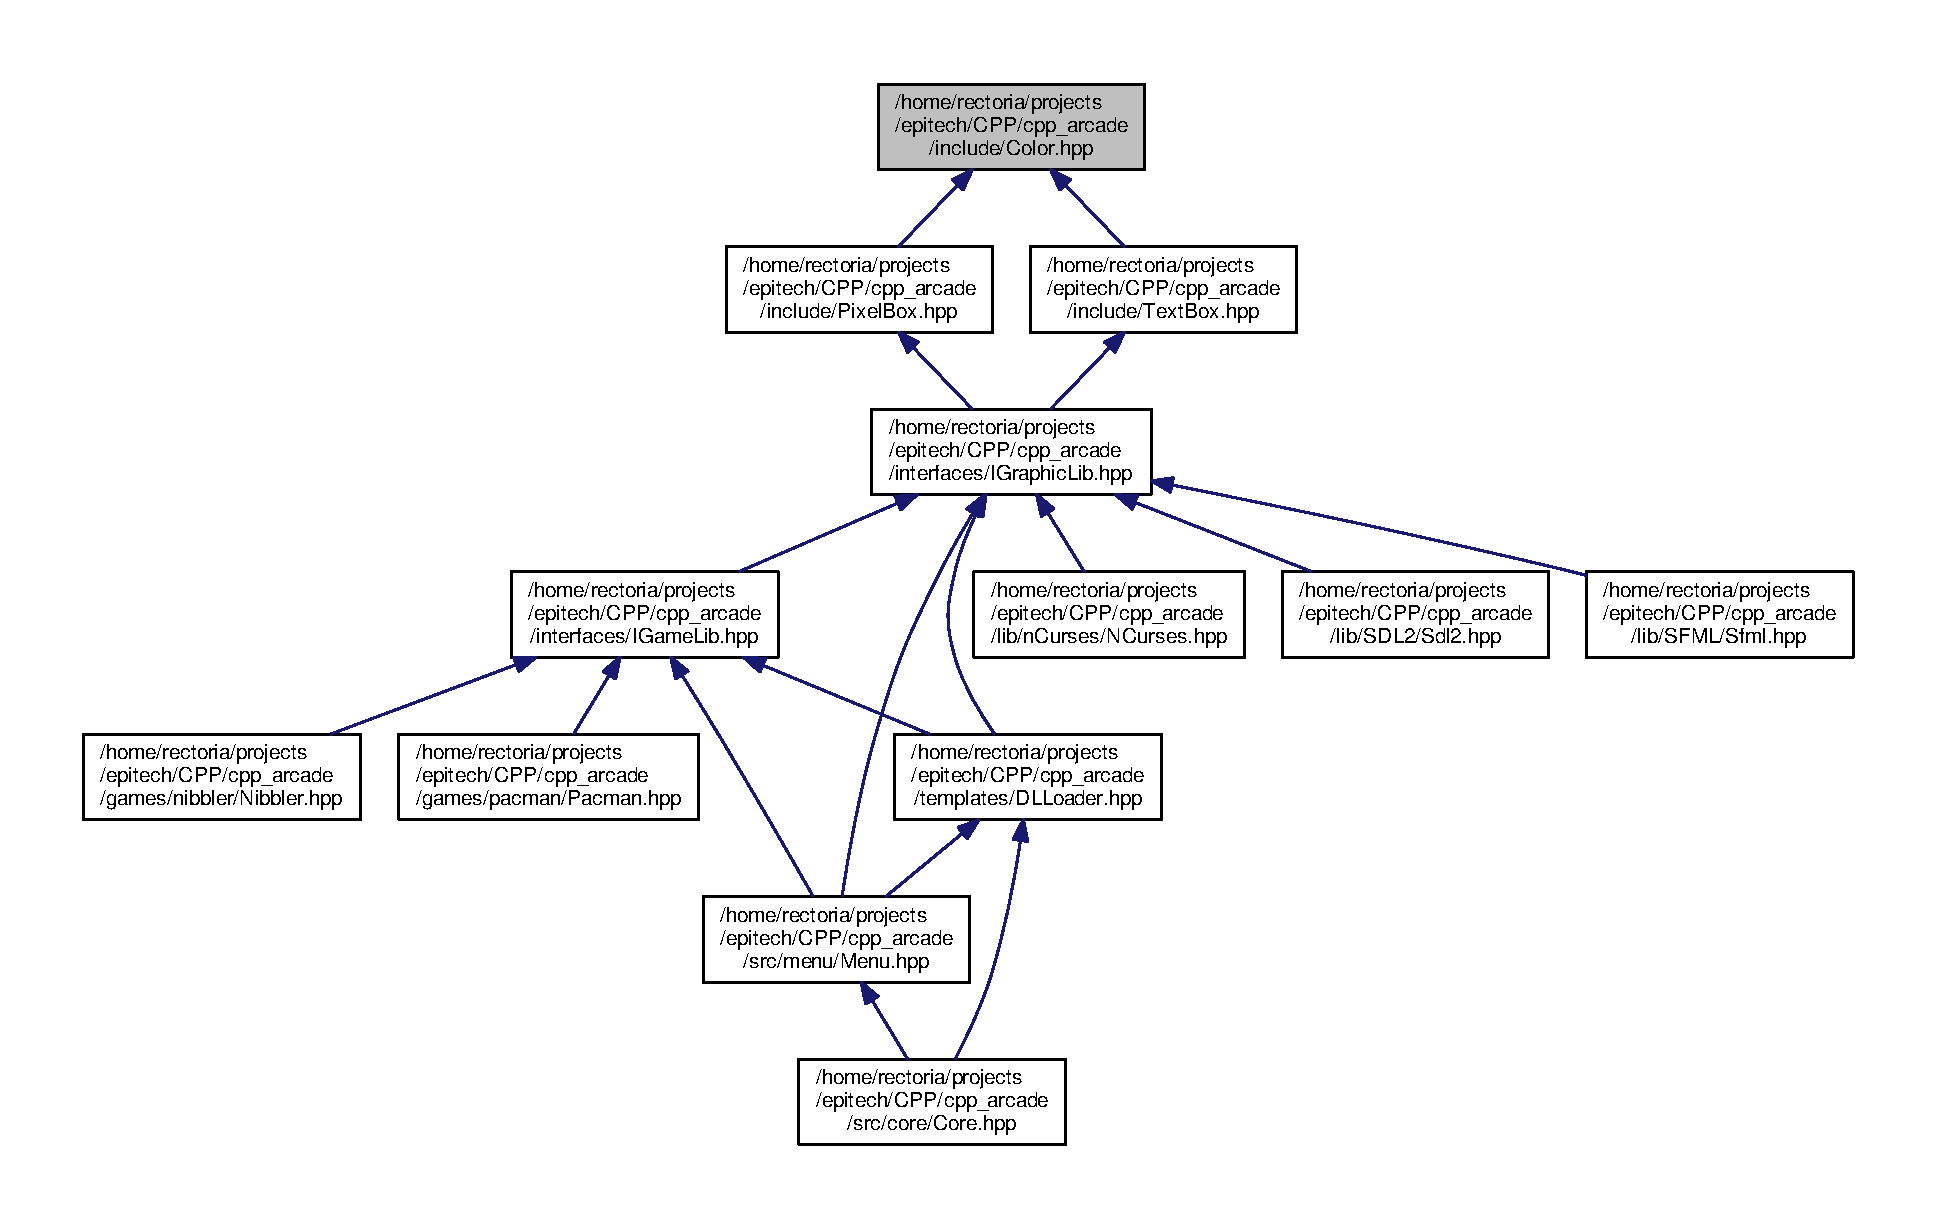
\includegraphics[width=350pt]{_color_8hpp__dep__incl}
\end{center}
\end{figure}
\subsection*{Classes}
\begin{DoxyCompactItemize}
\item 
class \hyperlink{class_arcade_1_1_color}{Arcade\+::\+Color}
\begin{DoxyCompactList}\small\item\em \hyperlink{class_arcade_1_1_color}{Color} class. \end{DoxyCompactList}\end{DoxyCompactItemize}
\subsection*{Namespaces}
\begin{DoxyCompactItemize}
\item 
 \hyperlink{namespace_arcade}{Arcade}
\begin{DoxyCompactList}\small\item\em \hyperlink{namespace_arcade}{Arcade} project namespace. \end{DoxyCompactList}\end{DoxyCompactItemize}


\subsection{Detailed Description}
Color class, pixel-\/like. 

\begin{DoxyAuthor}{Authors}
\href{https://github.com/EPITECH-Strasbourg-2021/CPP-Arcade-Spec}{\tt https\+://github.\+com/\+E\+P\+I\+T\+E\+C\+H-\/\+Strasbourg-\/2021/\+C\+P\+P-\/\+Arcade-\/\+Spec}
\end{DoxyAuthor}
Class used by games and graphic libraries, as a color\textquotesingle{}s array All functions must be implemented correctly for libraries to function properly. 
\hypertarget{_keys_8hpp}{}\section{/home/rectoria/projects/epitech/\+C\+P\+P/cpp\+\_\+arcade/include/\+Keys.hpp File Reference}
\label{_keys_8hpp}\index{/home/rectoria/projects/epitech/\+C\+P\+P/cpp\+\_\+arcade/include/\+Keys.\+hpp@{/home/rectoria/projects/epitech/\+C\+P\+P/cpp\+\_\+arcade/include/\+Keys.\+hpp}}


Keys enum.  


This graph shows which files directly or indirectly include this file\+:
\nopagebreak
\begin{figure}[H]
\begin{center}
\leavevmode
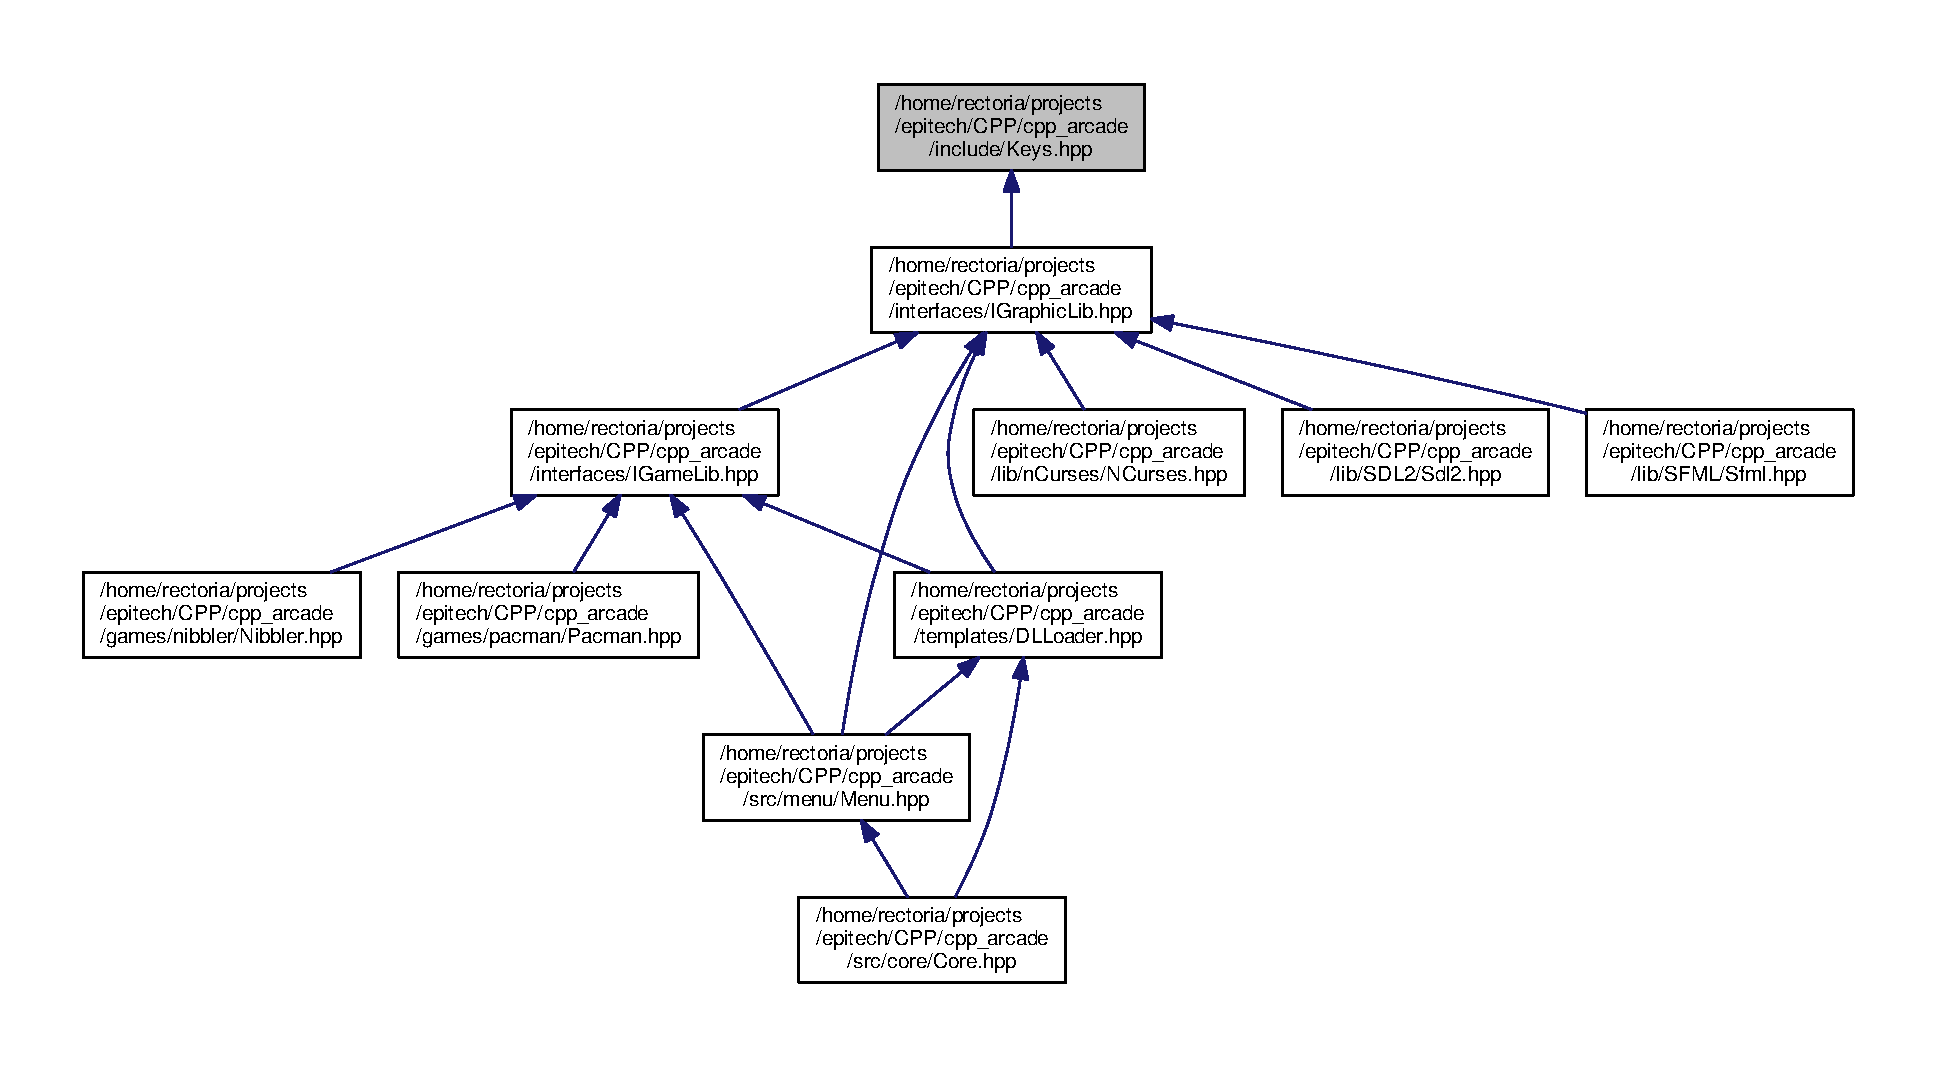
\includegraphics[width=350pt]{_keys_8hpp__dep__incl}
\end{center}
\end{figure}
\subsection*{Namespaces}
\begin{DoxyCompactItemize}
\item 
 \hyperlink{namespace_arcade}{Arcade}
\begin{DoxyCompactList}\small\item\em \hyperlink{namespace_arcade}{Arcade} project namespace. \end{DoxyCompactList}\end{DoxyCompactItemize}
\subsection*{Enumerations}
\begin{DoxyCompactItemize}
\item 
enum \hyperlink{namespace_arcade_a9b501908b20bc993e4f8226db5323c41}{Arcade\+::\+Keys} \{ \newline
{\bfseries N\+O\+NE}, 
{\bfseries A}, 
{\bfseries B}, 
{\bfseries C}, 
\newline
{\bfseries D}, 
{\bfseries E}, 
{\bfseries F}, 
{\bfseries G}, 
\newline
{\bfseries H}, 
{\bfseries I}, 
{\bfseries J}, 
{\bfseries K}, 
\newline
{\bfseries L}, 
{\bfseries M}, 
{\bfseries N}, 
{\bfseries O}, 
\newline
{\bfseries P}, 
{\bfseries Q}, 
{\bfseries R}, 
{\bfseries S}, 
\newline
{\bfseries T}, 
{\bfseries U}, 
{\bfseries V}, 
{\bfseries W}, 
\newline
{\bfseries X}, 
{\bfseries Y}, 
{\bfseries Z}, 
{\bfseries L\+E\+FT}, 
\newline
{\bfseries R\+I\+G\+HT}, 
{\bfseries UP}, 
{\bfseries D\+O\+WN}, 
{\bfseries E\+N\+T\+ER}, 
\newline
{\bfseries S\+P\+A\+CE}, 
{\bfseries D\+E\+L\+E\+TE}, 
{\bfseries B\+A\+C\+K\+S\+P\+A\+CE}, 
{\bfseries T\+AB}, 
\newline
{\bfseries E\+SC}, 
{\bfseries M\+O\+U\+S\+E\+L\+E\+FT}, 
{\bfseries M\+O\+U\+S\+E\+R\+I\+G\+HT}
 \}
\end{DoxyCompactItemize}


\subsection{Detailed Description}
Keys enum. 

\begin{DoxyAuthor}{Authors}
\href{https://github.com/EPITECH-Strasbourg-2021/CPP-Arcade-Spec}{\tt https\+://github.\+com/\+E\+P\+I\+T\+E\+C\+H-\/\+Strasbourg-\/2021/\+C\+P\+P-\/\+Arcade-\/\+Spec}
\end{DoxyAuthor}
Key Enum, each graphics library must store a map in order to convert the specific library key code into one of this enum code so that it can be used by other components independently of the graphics library. 
\hypertarget{_pixel_box_8hpp}{}\section{/home/rectoria/projects/epitech/\+C\+P\+P/cpp\+\_\+arcade/include/\+Pixel\+Box.hpp File Reference}
\label{_pixel_box_8hpp}\index{/home/rectoria/projects/epitech/\+C\+P\+P/cpp\+\_\+arcade/include/\+Pixel\+Box.\+hpp@{/home/rectoria/projects/epitech/\+C\+P\+P/cpp\+\_\+arcade/include/\+Pixel\+Box.\+hpp}}


Pixel\+Box class, similar to a rectangle of pixels.  


{\ttfamily \#include $<$string$>$}\newline
{\ttfamily \#include $<$vector$>$}\newline
{\ttfamily \#include \char`\"{}Color.\+hpp\char`\"{}}\newline
{\ttfamily \#include \char`\"{}Vect.\+hpp\char`\"{}}\newline
Include dependency graph for Pixel\+Box.\+hpp\+:
\nopagebreak
\begin{figure}[H]
\begin{center}
\leavevmode
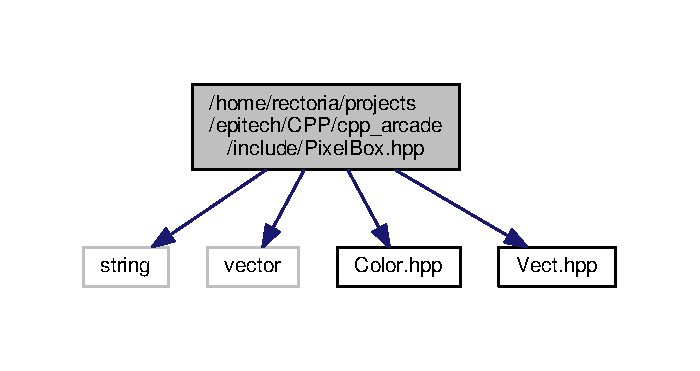
\includegraphics[width=336pt]{_pixel_box_8hpp__incl}
\end{center}
\end{figure}
This graph shows which files directly or indirectly include this file\+:
\nopagebreak
\begin{figure}[H]
\begin{center}
\leavevmode
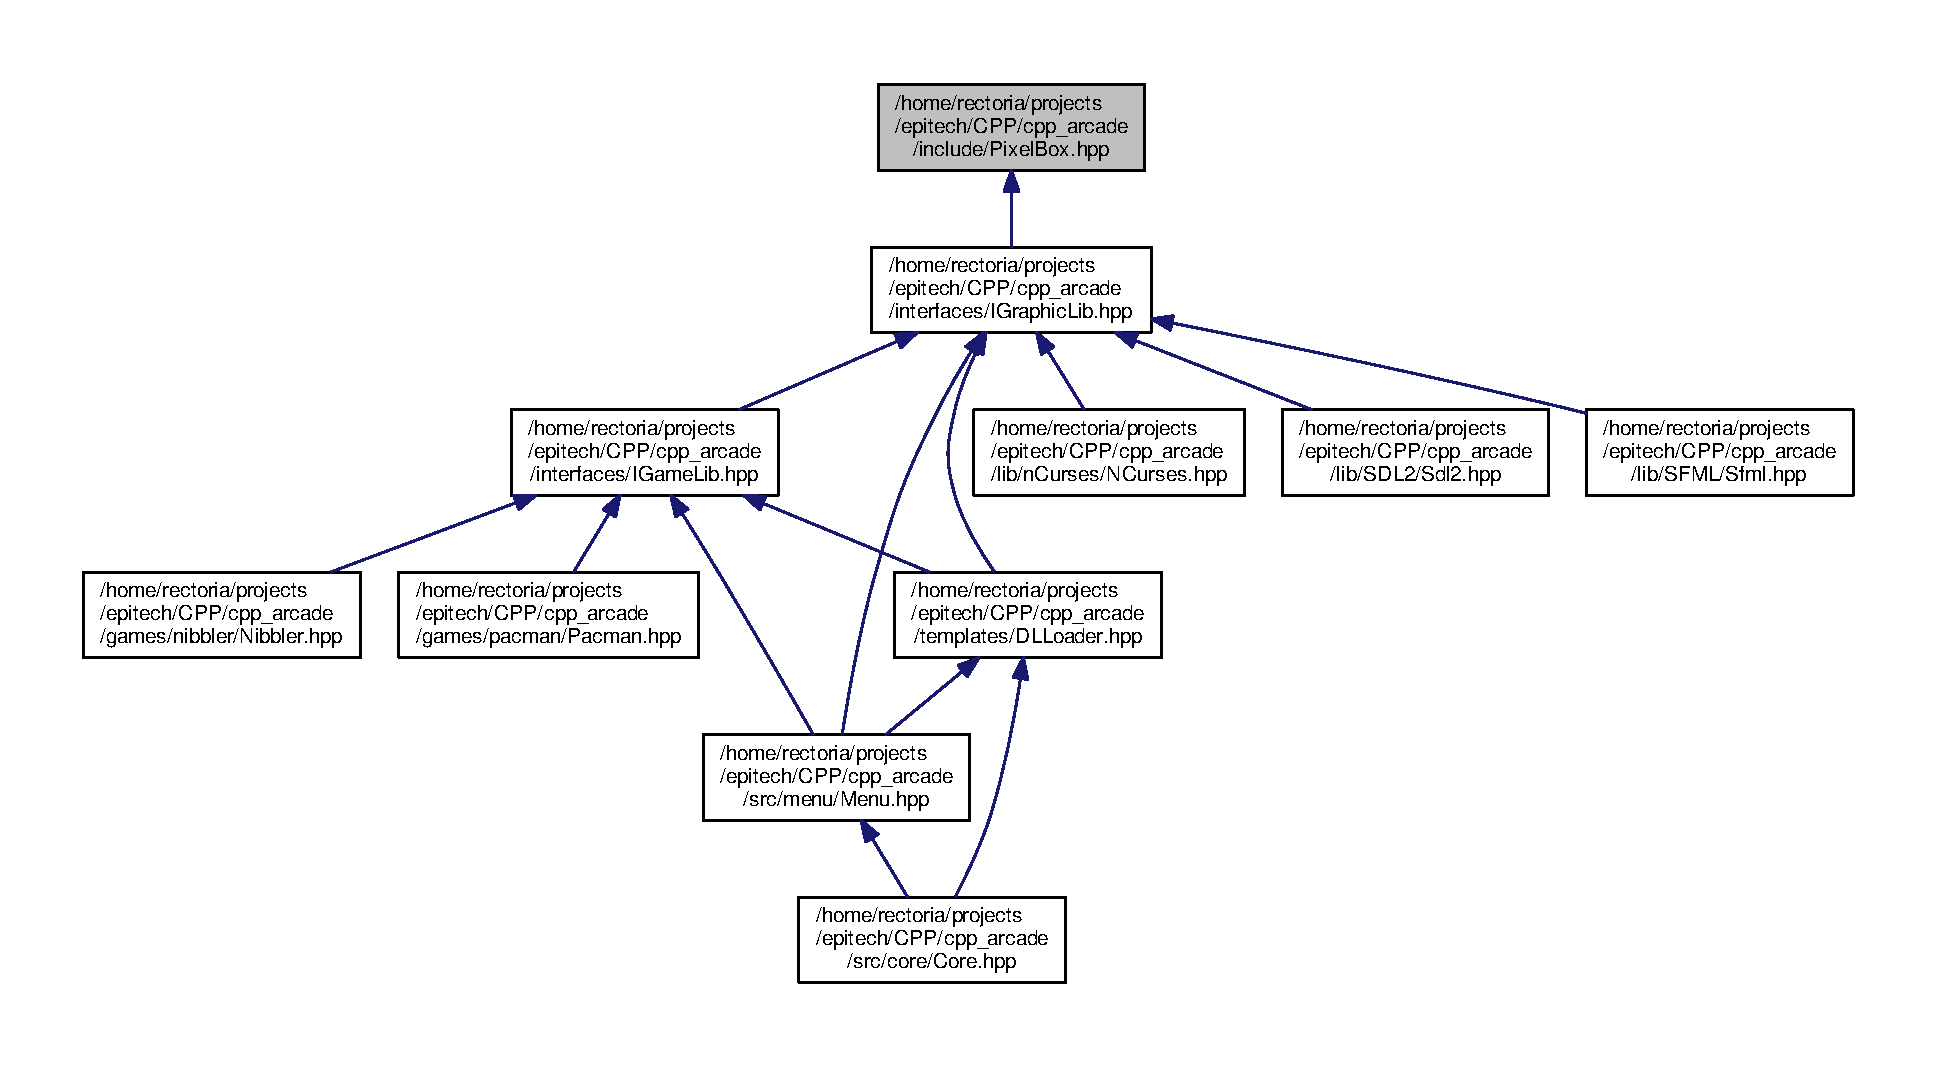
\includegraphics[width=350pt]{_pixel_box_8hpp__dep__incl}
\end{center}
\end{figure}
\subsection*{Classes}
\begin{DoxyCompactItemize}
\item 
class \hyperlink{class_arcade_1_1_pixel_box}{Arcade\+::\+Pixel\+Box}
\begin{DoxyCompactList}\small\item\em \hyperlink{class_arcade_1_1_pixel_box}{Pixel\+Box} class. \end{DoxyCompactList}\end{DoxyCompactItemize}
\subsection*{Namespaces}
\begin{DoxyCompactItemize}
\item 
 \hyperlink{namespace_arcade}{Arcade}
\begin{DoxyCompactList}\small\item\em \hyperlink{namespace_arcade}{Arcade} project namespace. \end{DoxyCompactList}\end{DoxyCompactItemize}


\subsection{Detailed Description}
Pixel\+Box class, similar to a rectangle of pixels. 

\begin{DoxyAuthor}{Authors}
\href{https://github.com/EPITECH-Strasbourg-2021/CPP-Arcade-Spec}{\tt https\+://github.\+com/\+E\+P\+I\+T\+E\+C\+H-\/\+Strasbourg-\/2021/\+C\+P\+P-\/\+Arcade-\/\+Spec}
\end{DoxyAuthor}
Class used by games and graphic libraries, similar to a rectangle of pixels. All functions must be implemented correctly for libraries to function properly. 
\hypertarget{_text_box_8hpp}{}\section{/home/rectoria/projects/epitech/\+C\+P\+P/cpp\+\_\+arcade/include/\+Text\+Box.hpp File Reference}
\label{_text_box_8hpp}\index{/home/rectoria/projects/epitech/\+C\+P\+P/cpp\+\_\+arcade/include/\+Text\+Box.\+hpp@{/home/rectoria/projects/epitech/\+C\+P\+P/cpp\+\_\+arcade/include/\+Text\+Box.\+hpp}}


Text\+Box class, similar to a text rectangle.  


{\ttfamily \#include $<$string$>$}\newline
{\ttfamily \#include \char`\"{}Color.\+hpp\char`\"{}}\newline
{\ttfamily \#include \char`\"{}Vect.\+hpp\char`\"{}}\newline
Include dependency graph for Text\+Box.\+hpp\+:
\nopagebreak
\begin{figure}[H]
\begin{center}
\leavevmode
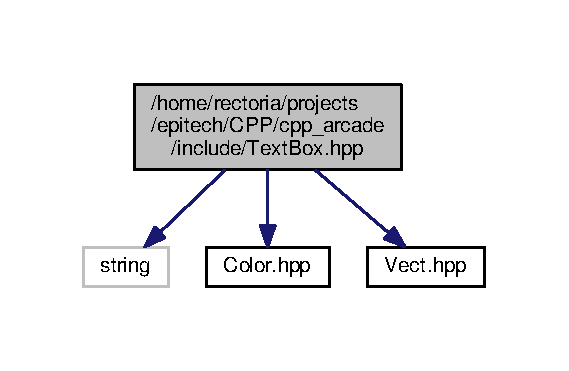
\includegraphics[width=273pt]{_text_box_8hpp__incl}
\end{center}
\end{figure}
This graph shows which files directly or indirectly include this file\+:
\nopagebreak
\begin{figure}[H]
\begin{center}
\leavevmode
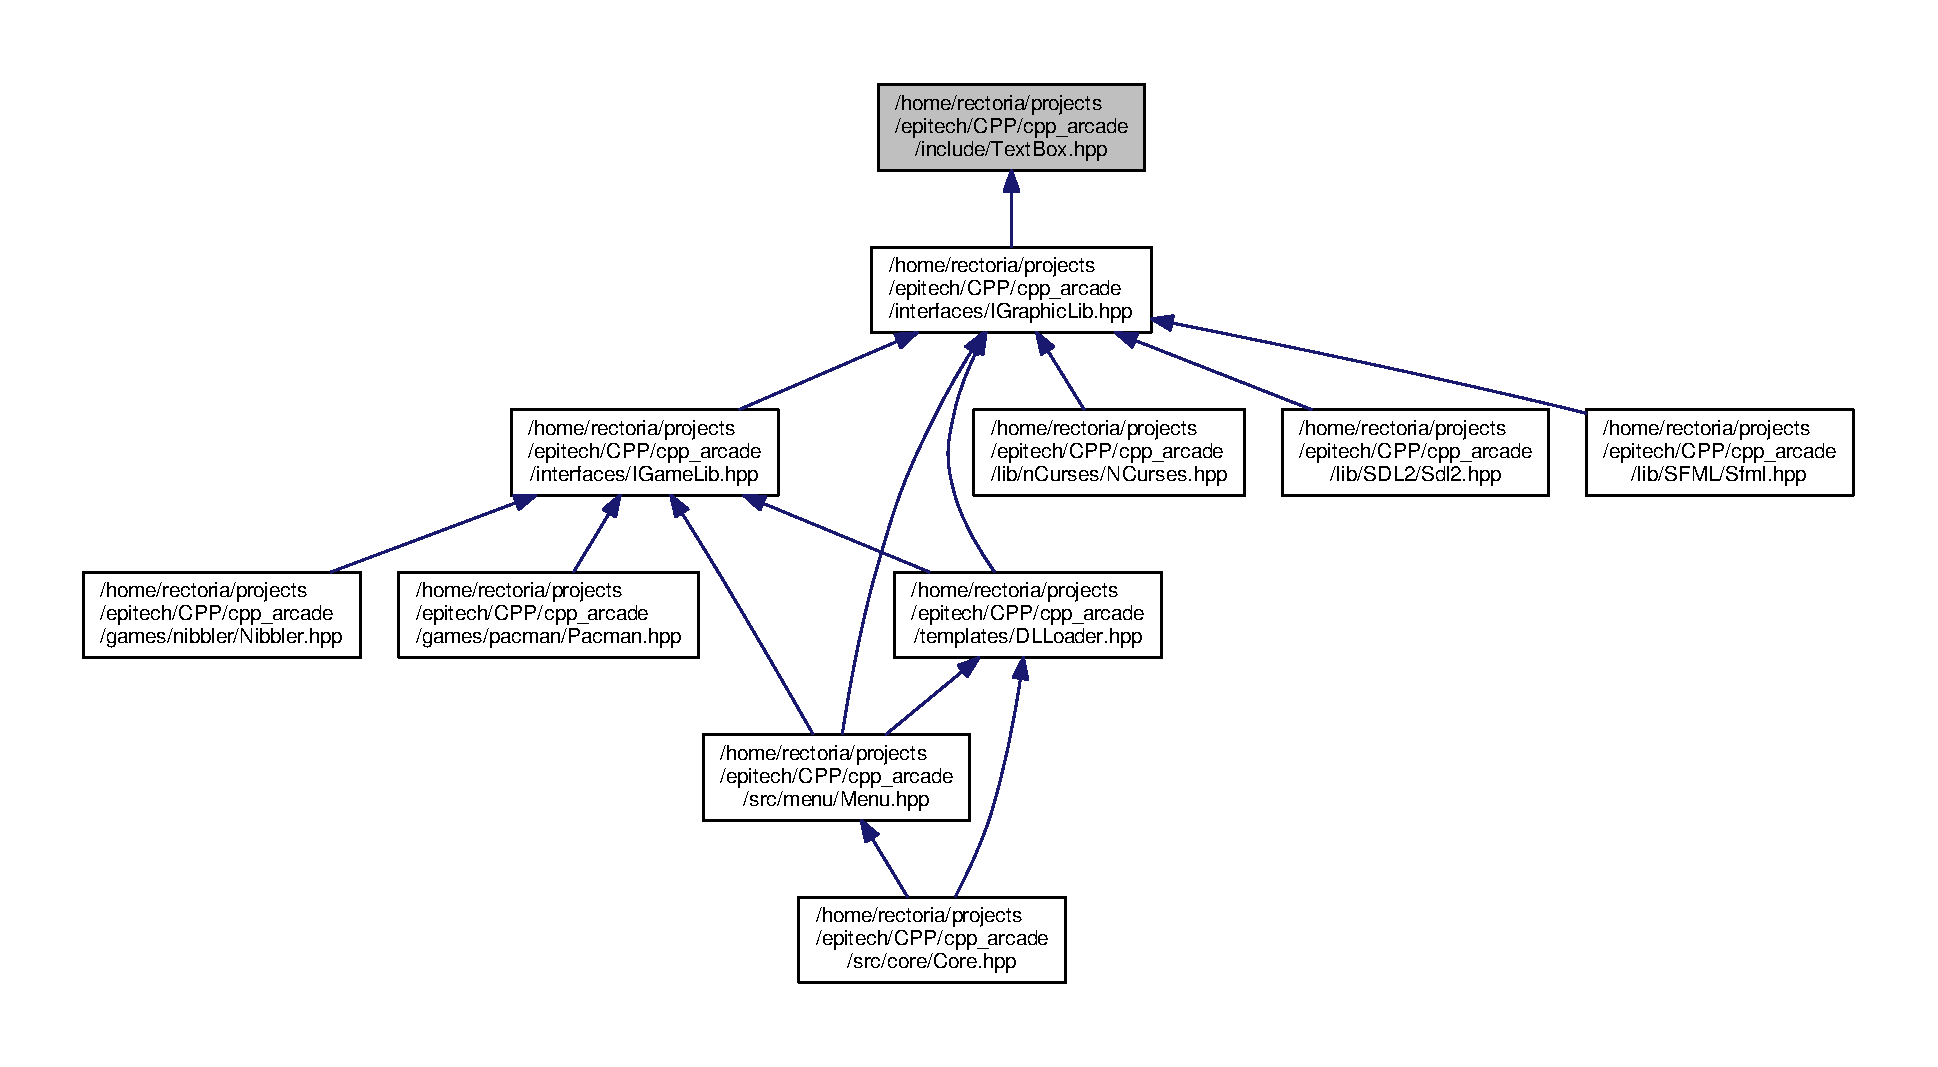
\includegraphics[width=350pt]{_text_box_8hpp__dep__incl}
\end{center}
\end{figure}
\subsection*{Classes}
\begin{DoxyCompactItemize}
\item 
class \hyperlink{class_arcade_1_1_text_box}{Arcade\+::\+Text\+Box}
\begin{DoxyCompactList}\small\item\em \hyperlink{class_arcade_1_1_text_box}{Text\+Box} class. \end{DoxyCompactList}\end{DoxyCompactItemize}
\subsection*{Namespaces}
\begin{DoxyCompactItemize}
\item 
 \hyperlink{namespace_arcade}{Arcade}
\begin{DoxyCompactList}\small\item\em \hyperlink{namespace_arcade}{Arcade} project namespace. \end{DoxyCompactList}\end{DoxyCompactItemize}


\subsection{Detailed Description}
Text\+Box class, similar to a text rectangle. 

\begin{DoxyAuthor}{Authors}
\href{https://github.com/EPITECH-Strasbourg-2021/CPP-Arcade-Spec}{\tt https\+://github.\+com/\+E\+P\+I\+T\+E\+C\+H-\/\+Strasbourg-\/2021/\+C\+P\+P-\/\+Arcade-\/\+Spec}
\end{DoxyAuthor}
Class used by games and graphic libraries, similar to a text rectangle. All functions must be implemented correctly for libraries to function properly. 
\hypertarget{_vect_8hpp}{}\section{/home/rectoria/projects/epitech/\+C\+P\+P/cpp\+\_\+arcade/include/\+Vect.hpp File Reference}
\label{_vect_8hpp}\index{/home/rectoria/projects/epitech/\+C\+P\+P/cpp\+\_\+arcade/include/\+Vect.\+hpp@{/home/rectoria/projects/epitech/\+C\+P\+P/cpp\+\_\+arcade/include/\+Vect.\+hpp}}


Project-\/specific vector template.  


This graph shows which files directly or indirectly include this file\+:
\nopagebreak
\begin{figure}[H]
\begin{center}
\leavevmode
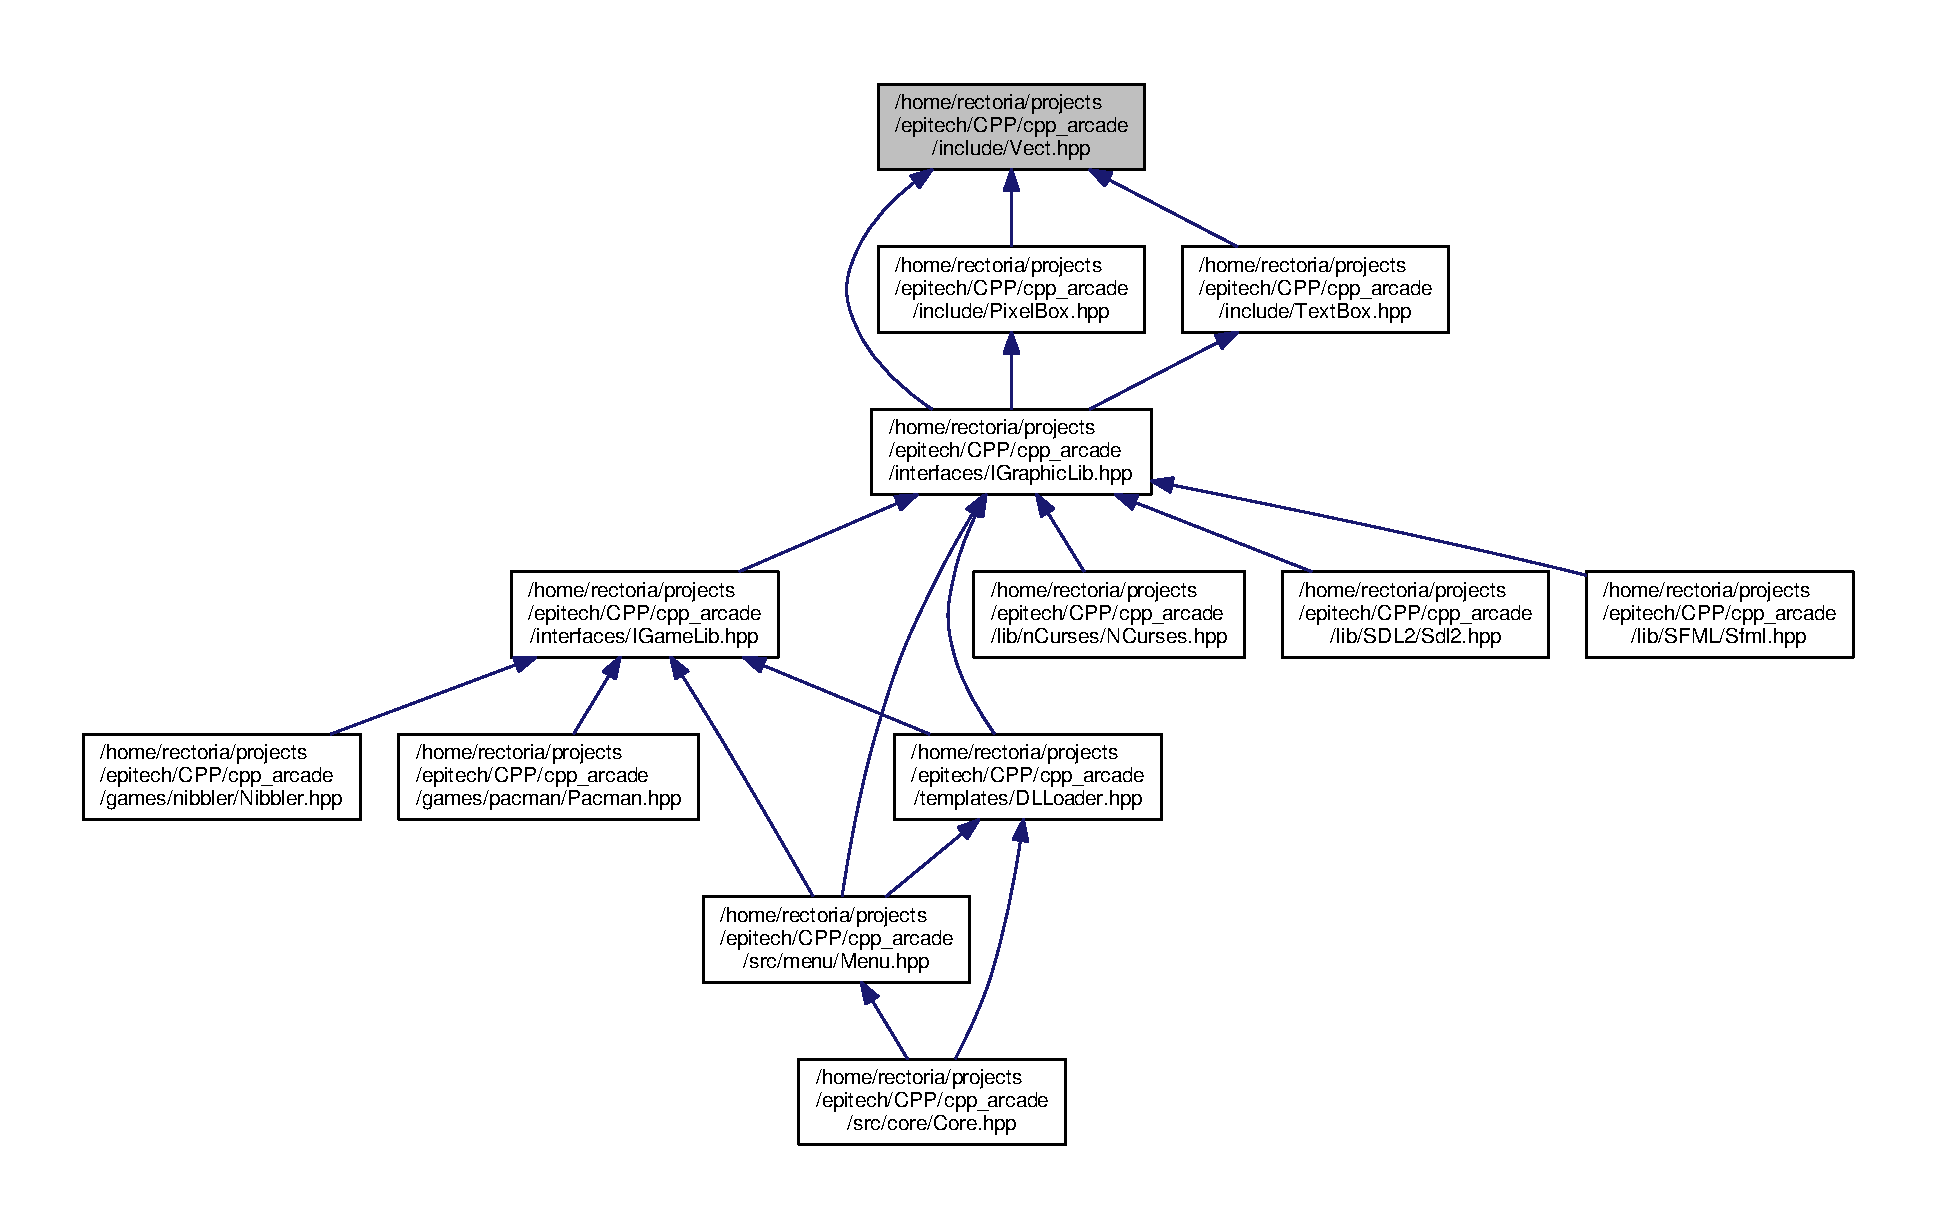
\includegraphics[width=350pt]{_vect_8hpp__dep__incl}
\end{center}
\end{figure}
\subsection*{Classes}
\begin{DoxyCompactItemize}
\item 
class \hyperlink{class_arcade_1_1_vect}{Arcade\+::\+Vect$<$ T $>$}
\begin{DoxyCompactList}\small\item\em \hyperlink{class_arcade_1_1_vect}{Vect} class template. \end{DoxyCompactList}\end{DoxyCompactItemize}
\subsection*{Namespaces}
\begin{DoxyCompactItemize}
\item 
 \hyperlink{namespace_arcade}{Arcade}
\begin{DoxyCompactList}\small\item\em \hyperlink{namespace_arcade}{Arcade} project namespace. \end{DoxyCompactList}\end{DoxyCompactItemize}


\subsection{Detailed Description}
Project-\/specific vector template. 

\begin{DoxyAuthor}{Authors}
\href{https://github.com/EPITECH-Strasbourg-2021/CPP-Arcade-Spec}{\tt https\+://github.\+com/\+E\+P\+I\+T\+E\+C\+H-\/\+Strasbourg-\/2021/\+C\+P\+P-\/\+Arcade-\/\+Spec}
\end{DoxyAuthor}
Template used to store and perform arithmetic operations on coordinates. 
\hypertarget{_i_game_lib_8hpp}{}\section{/home/rectoria/projects/epitech/\+C\+P\+P/cpp\+\_\+arcade/interfaces/\+I\+Game\+Lib.hpp File Reference}
\label{_i_game_lib_8hpp}\index{/home/rectoria/projects/epitech/\+C\+P\+P/cpp\+\_\+arcade/interfaces/\+I\+Game\+Lib.\+hpp@{/home/rectoria/projects/epitech/\+C\+P\+P/cpp\+\_\+arcade/interfaces/\+I\+Game\+Lib.\+hpp}}


Game libraries dedicated class interface.  


{\ttfamily \#include \char`\"{}I\+Graphic\+Lib.\+hpp\char`\"{}}\newline
Include dependency graph for I\+Game\+Lib.\+hpp\+:
\nopagebreak
\begin{figure}[H]
\begin{center}
\leavevmode
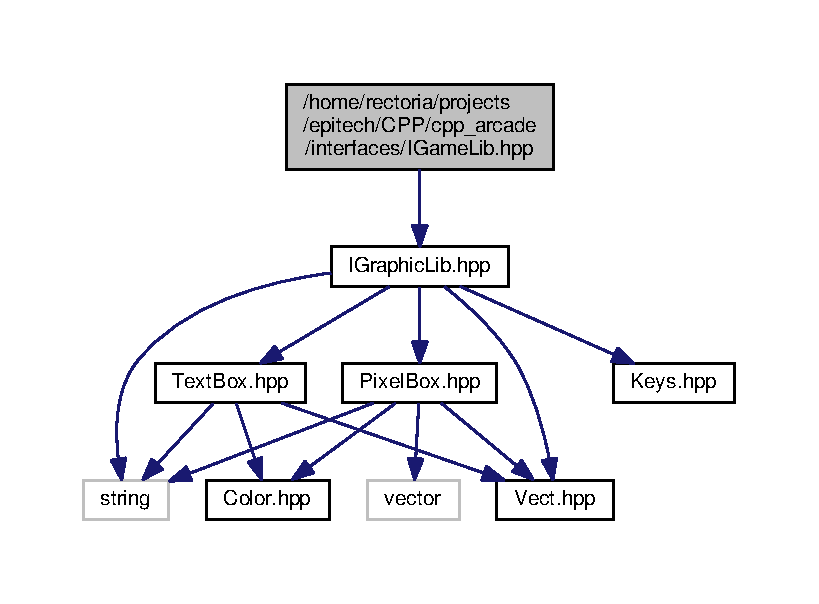
\includegraphics[width=350pt]{_i_game_lib_8hpp__incl}
\end{center}
\end{figure}
This graph shows which files directly or indirectly include this file\+:
\nopagebreak
\begin{figure}[H]
\begin{center}
\leavevmode
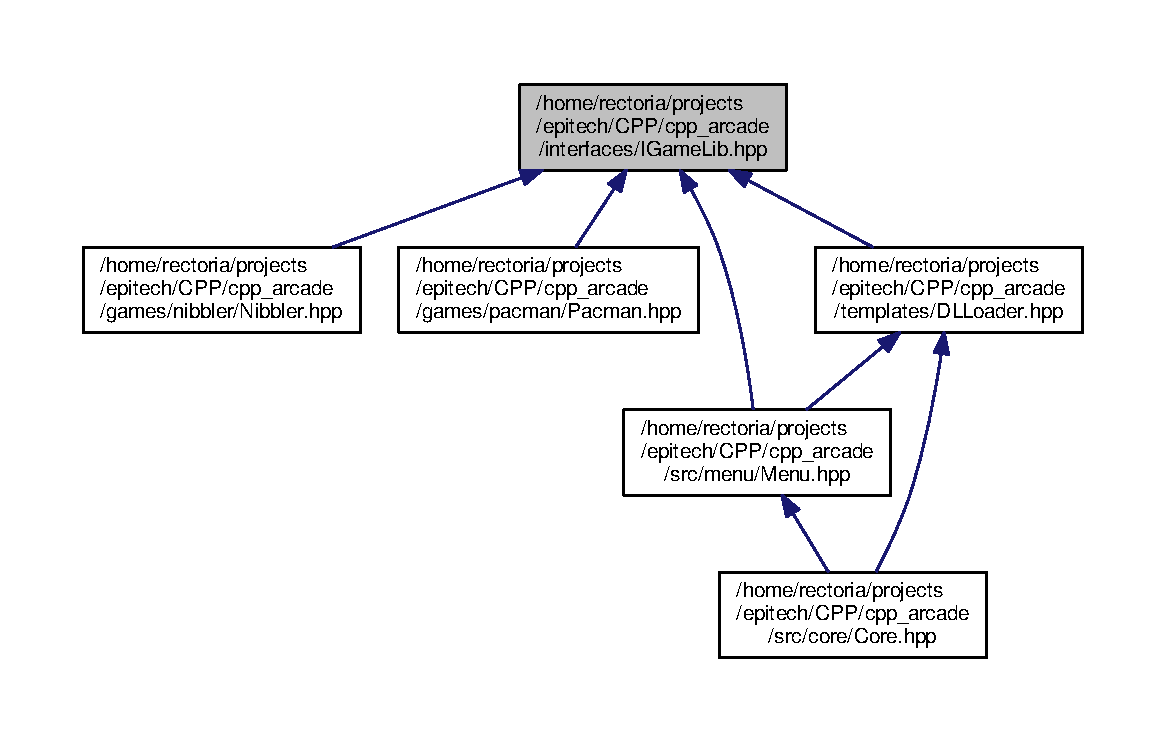
\includegraphics[width=350pt]{_i_game_lib_8hpp__dep__incl}
\end{center}
\end{figure}
\subsection*{Classes}
\begin{DoxyCompactItemize}
\item 
class \hyperlink{class_arcade_1_1_i_game_lib}{Arcade\+::\+I\+Game\+Lib}
\begin{DoxyCompactList}\small\item\em Game libraries virtual class. \end{DoxyCompactList}\end{DoxyCompactItemize}
\subsection*{Namespaces}
\begin{DoxyCompactItemize}
\item 
 \hyperlink{namespace_arcade}{Arcade}
\begin{DoxyCompactList}\small\item\em \hyperlink{namespace_arcade}{Arcade} project namespace. \end{DoxyCompactList}\end{DoxyCompactItemize}


\subsection{Detailed Description}
Game libraries dedicated class interface. 

\begin{DoxyAuthor}{Authors}
\href{https://github.com/EPITECH-Strasbourg-2021/CPP-Arcade-Spec}{\tt https\+://github.\+com/\+E\+P\+I\+T\+E\+C\+H-\/\+Strasbourg-\/2021/\+C\+P\+P-\/\+Arcade-\/\+Spec}
\end{DoxyAuthor}
Interface used by game libraries. All functions must be implemented correctly for the kernel to handle the game libraries. 
\hypertarget{_i_graphic_lib_8hpp}{}\section{/home/rectoria/projects/epitech/\+C\+P\+P/cpp\+\_\+arcade/interfaces/\+I\+Graphic\+Lib.hpp File Reference}
\label{_i_graphic_lib_8hpp}\index{/home/rectoria/projects/epitech/\+C\+P\+P/cpp\+\_\+arcade/interfaces/\+I\+Graphic\+Lib.\+hpp@{/home/rectoria/projects/epitech/\+C\+P\+P/cpp\+\_\+arcade/interfaces/\+I\+Graphic\+Lib.\+hpp}}


Graphic libraries dedicated class interface.  


{\ttfamily \#include $<$string$>$}\newline
{\ttfamily \#include \char`\"{}Vect.\+hpp\char`\"{}}\newline
{\ttfamily \#include \char`\"{}Pixel\+Box.\+hpp\char`\"{}}\newline
{\ttfamily \#include \char`\"{}Text\+Box.\+hpp\char`\"{}}\newline
{\ttfamily \#include \char`\"{}Keys.\+hpp\char`\"{}}\newline
Include dependency graph for I\+Graphic\+Lib.\+hpp\+:
\nopagebreak
\begin{figure}[H]
\begin{center}
\leavevmode
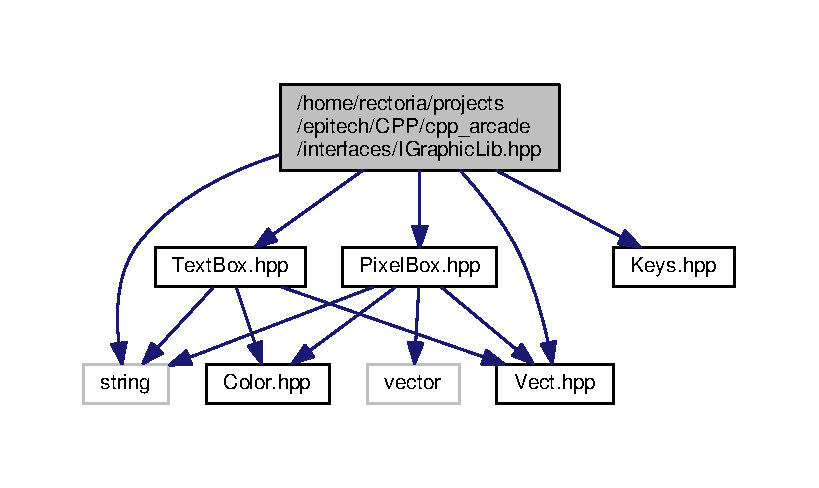
\includegraphics[width=350pt]{_i_graphic_lib_8hpp__incl}
\end{center}
\end{figure}
This graph shows which files directly or indirectly include this file\+:
\nopagebreak
\begin{figure}[H]
\begin{center}
\leavevmode
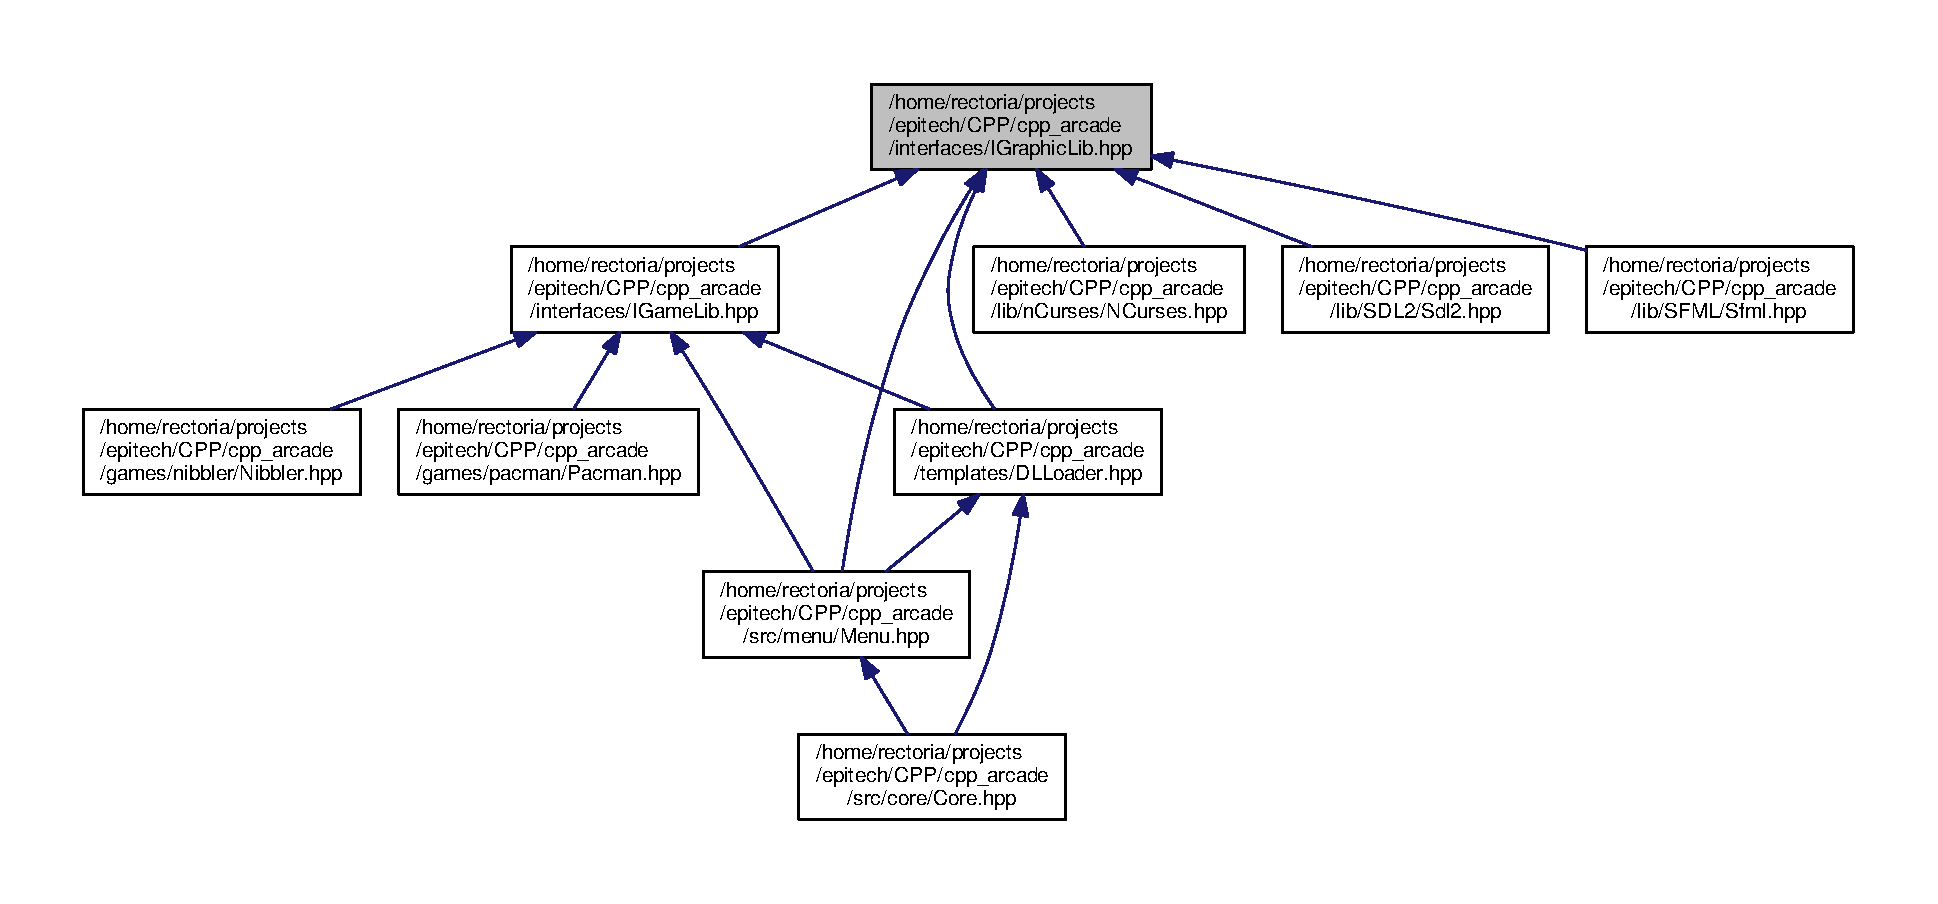
\includegraphics[width=350pt]{_i_graphic_lib_8hpp__dep__incl}
\end{center}
\end{figure}
\subsection*{Classes}
\begin{DoxyCompactItemize}
\item 
class \hyperlink{class_arcade_1_1_i_graphic_lib}{Arcade\+::\+I\+Graphic\+Lib}
\begin{DoxyCompactList}\small\item\em Graphic libraries virtual class. \end{DoxyCompactList}\end{DoxyCompactItemize}
\subsection*{Namespaces}
\begin{DoxyCompactItemize}
\item 
 \hyperlink{namespace_arcade}{Arcade}
\begin{DoxyCompactList}\small\item\em \hyperlink{namespace_arcade}{Arcade} project namespace. \end{DoxyCompactList}\end{DoxyCompactItemize}


\subsection{Detailed Description}
Graphic libraries dedicated class interface. 

\begin{DoxyAuthor}{Authors}
\href{https://github.com/EPITECH-Strasbourg-2021/CPP-Arcade-Spec}{\tt https\+://github.\+com/\+E\+P\+I\+T\+E\+C\+H-\/\+Strasbourg-\/2021/\+C\+P\+P-\/\+Arcade-\/\+Spec}
\end{DoxyAuthor}
Interface used by graphic libraries All functions must be implemented correctly for the kernel to handle the graphic libraries. 
%--- End generated contents ---

% Index
\backmatter
\newpage
\phantomsection
\clearemptydoublepage
\addcontentsline{toc}{chapter}{Index}
\printindex

\end{document}
